\documentclass[a4paper,11pt]{article}

\usepackage[T1]{fontenc}        % poprawne łamanie polskich znaków
\usepackage{lmodern}
\usepackage[utf8]{inputenc}     % kodowanie UTF-8
\usepackage[polish]{babel}      % język polski (nowocześniej niż \usepackage{polski})
\usepackage{microtype}

\usepackage{listings}

\setlength{\headheight}{16pt}
\usepackage{enumerate}
\usepackage{float}

\usepackage{amssymb}		% pakiet do symboli
\usepackage{amsmath}		% pakiet do matmy

\usepackage{microtype}          % lepsze łamanie wierszy (bardzo polecane)
\usepackage[a4paper, margin=1.5cm, top=2cm, bottom=1.8cm]{geometry}

\usepackage{enumerate}
\usepackage{wrapfig} % enables wrapfigure environment
\usepackage{subcaption} % for subfigure environment
\usepackage{enumitem}		% punktowanie (a), (b), ...

\usepackage{graphicx}		% wstawianie obrazkow
\usepackage{float}			% wstawianie obrazkow w dowolnym miejscu
% \usepackage{tabstackengine} 	% macierze
\usepackage{fancyhdr}		% ładniejszy wygląd stronki
% \usepackage{color}   		% kolorowanie linków / odnośników
\usepackage{hyperref} %do linków
\hypersetup{
    colorlinks=true, 	% set true if you want colored links
    linktoc=all,     	% set to all if you want both sections and subsections linked
    linkcolor=black,  	% choose some color if you want links to stand out
}
\usepackage{titling}

\usepackage{tcolorbox}
\usepackage{listings}   % do ładnego kodu/regexów

\usepackage{newclude}
\usepackage{xinttools}
\usepackage{color}

\usepackage[a4paper, margin=1.5cm, top=2cm, bottom=1.8cm]{geometry}


% for + / -
\usepackage{tikz}
\newcommand{\Mypm}{\mathbin{\tikz [x=1.4ex,y=1.4ex,line width=.1ex] \draw (0.0,0) -- (1.0,0) (0.5,0.08) -- (0.5,0.92) (0.0,0.5) -- (1.0,0.5);}}%


\renewcommand\labelitemi{\raisebox{-0.3ex}{\huge\boldmath$\cdot$}} % obniżenie pkt + zmniejszenie
% przeciwko dzieleniu słów np bez- (enter) względny
\hyphenpenalty=10000
\exhyphenpenalty=10000

% \stackMath

% nowe komendy dla wygodniejszego pisania :)
\newcommand{\subtitle}[1]{ \posttitle{ \par\end{center} \begin{center}\large#1\end{center} \vskip0.5em}}
% \newcommand{\floor}[1]{\left\lfloor #1 \right\rfloor}
\newcommand{\ceil}[1]{\left\lceil #1 \right\rceil}

% Wyglad strony:
% \pagestyle{fancy}
\fancyhf{}
\chead{\leftmark}
\cfoot{\thepage}

%%%%%%%%%%%%%%%%%%%%%%%%%%%%%%%%%%%%%%%%%%%%%%%%%%%%%%%%%%%%%%%%%%%%%

% \author{}
\title{\textbf{VAE}\\
Raport from project}
\author{Autor: Kamila Korczyńska\textbf{}}



% \subtitle{Redukcja}
\date{}

%%%%%%%%%%%%%%%%%%%%%%%%%%%%%%%%%%%%%%%%%%%%%%%%%%%%%%%%%%%%%%%%%%%%%
\begin{document}
\thispagestyle{empty}
\maketitle
\mbox{}

\section{Dataset}
The model is trained on the Cat Dataset from Kaggle:\\
https://www.kaggle.com/datasets/dimensi0n/afhq-512?select=cat\\

The dataset contains cat images, which are resized (64x64 RGB) and used as unsupervised training data.\\
Unfortunately, the dataset had series of photos witch could lead to data leakage, to resolve that problem we used Dinov2 to recognise "too similar" photos. 

\section{Implementation of Basic VAE Architectures}

Several VAE architectures were implemented:

\begin{itemize}
    \item a simple MLP VAE,
    \item a CNN VAE with a vector latent representation,
    \item a CNN VAE with a spatial latent representation.
\end{itemize}

The CNN VAE with a vector latent representation became the main architecture used in later experiments.

The standard VAE reparameterization mechanism was implemented:

\[
z = \mu + \sigma \epsilon,
\qquad
\epsilon \sim \mathcal{N}(0,I).
\]

The KL divergence between the approximate posterior and the standard normal prior was also implemented.

\subsection{MLP VAE}
\subsection{CNN VAE with a vector latent representation}

\begin{figure}[H]
    \centering

    \begin{subfigure}{0.48\textwidth}
        \centering
        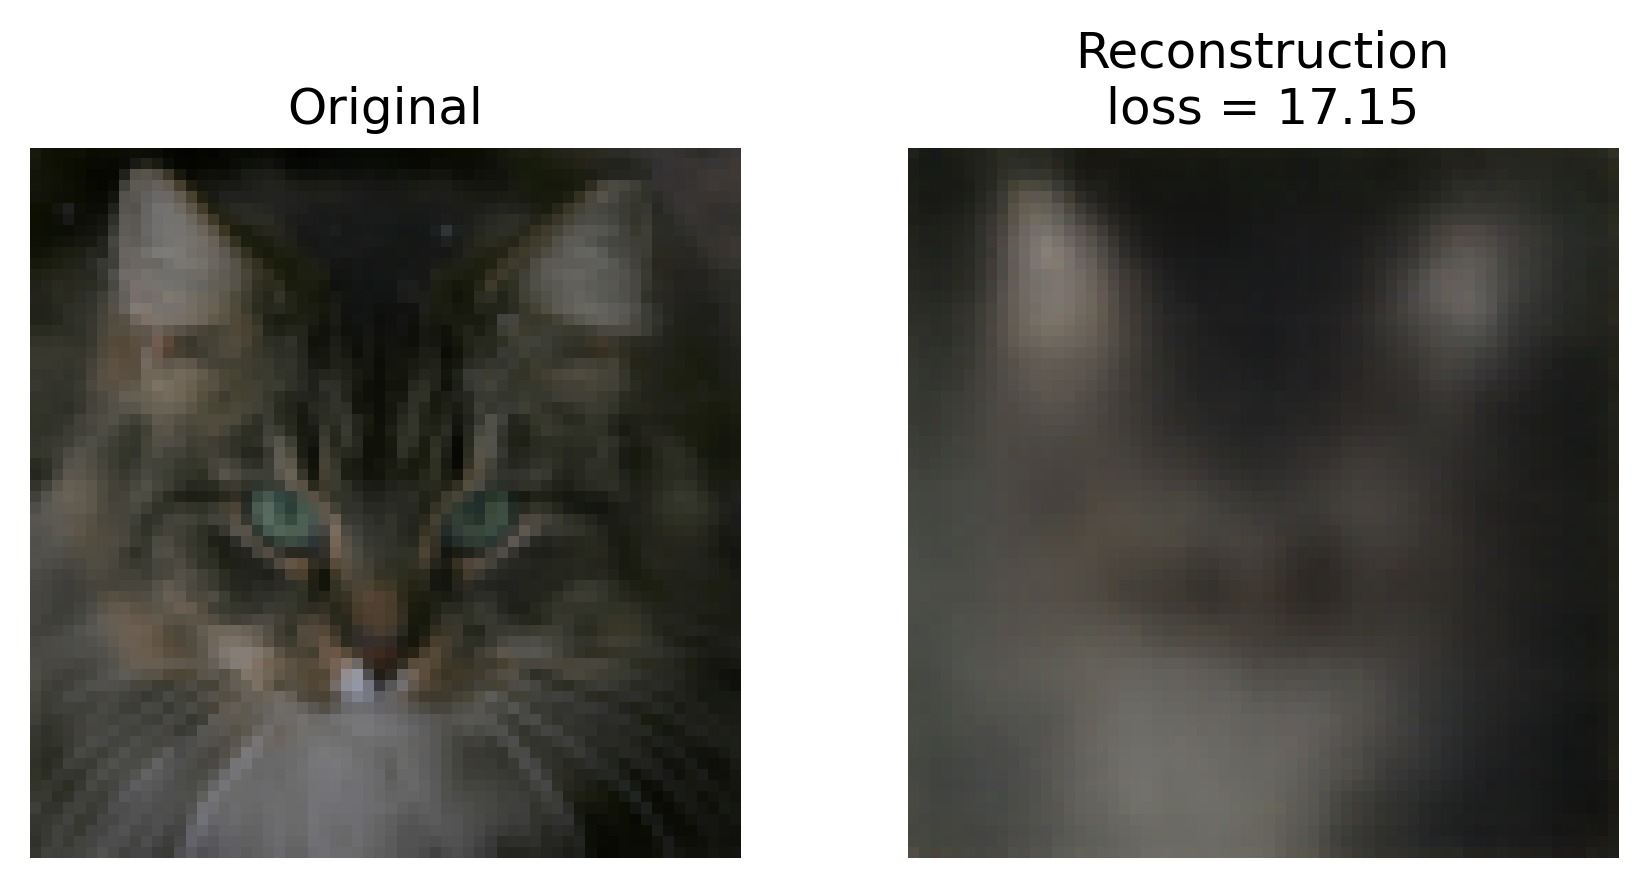
\includegraphics[width=\linewidth]{vector_latent/VAE/train_best_0.png}
        \caption*{}
    \end{subfigure}
    \hspace{0.02\textwidth}
    \begin{subfigure}{0.48\textwidth}
        \centering
        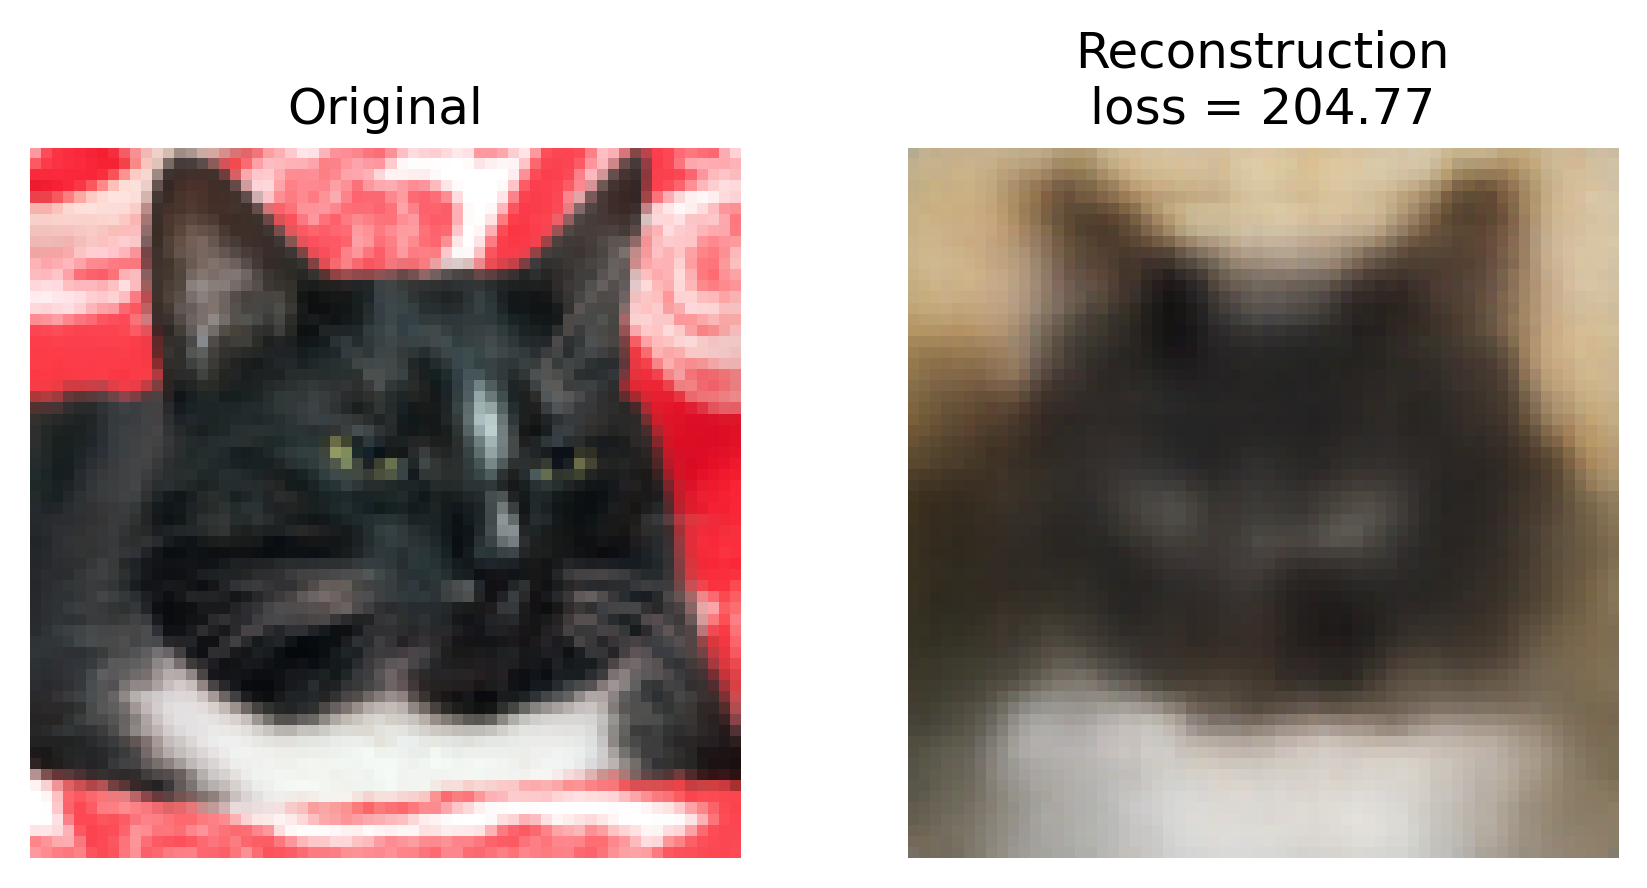
\includegraphics[width=\linewidth]{vector_latent/VAE/val_worst_2.png}
        \caption*{}
    \end{subfigure}

    \caption{Examples of reconstruction quality for the vector latent VAE.}
    \label{fig:spatial_latent_examples}
\end{figure}


\begin{figure}[H]
    \centering
    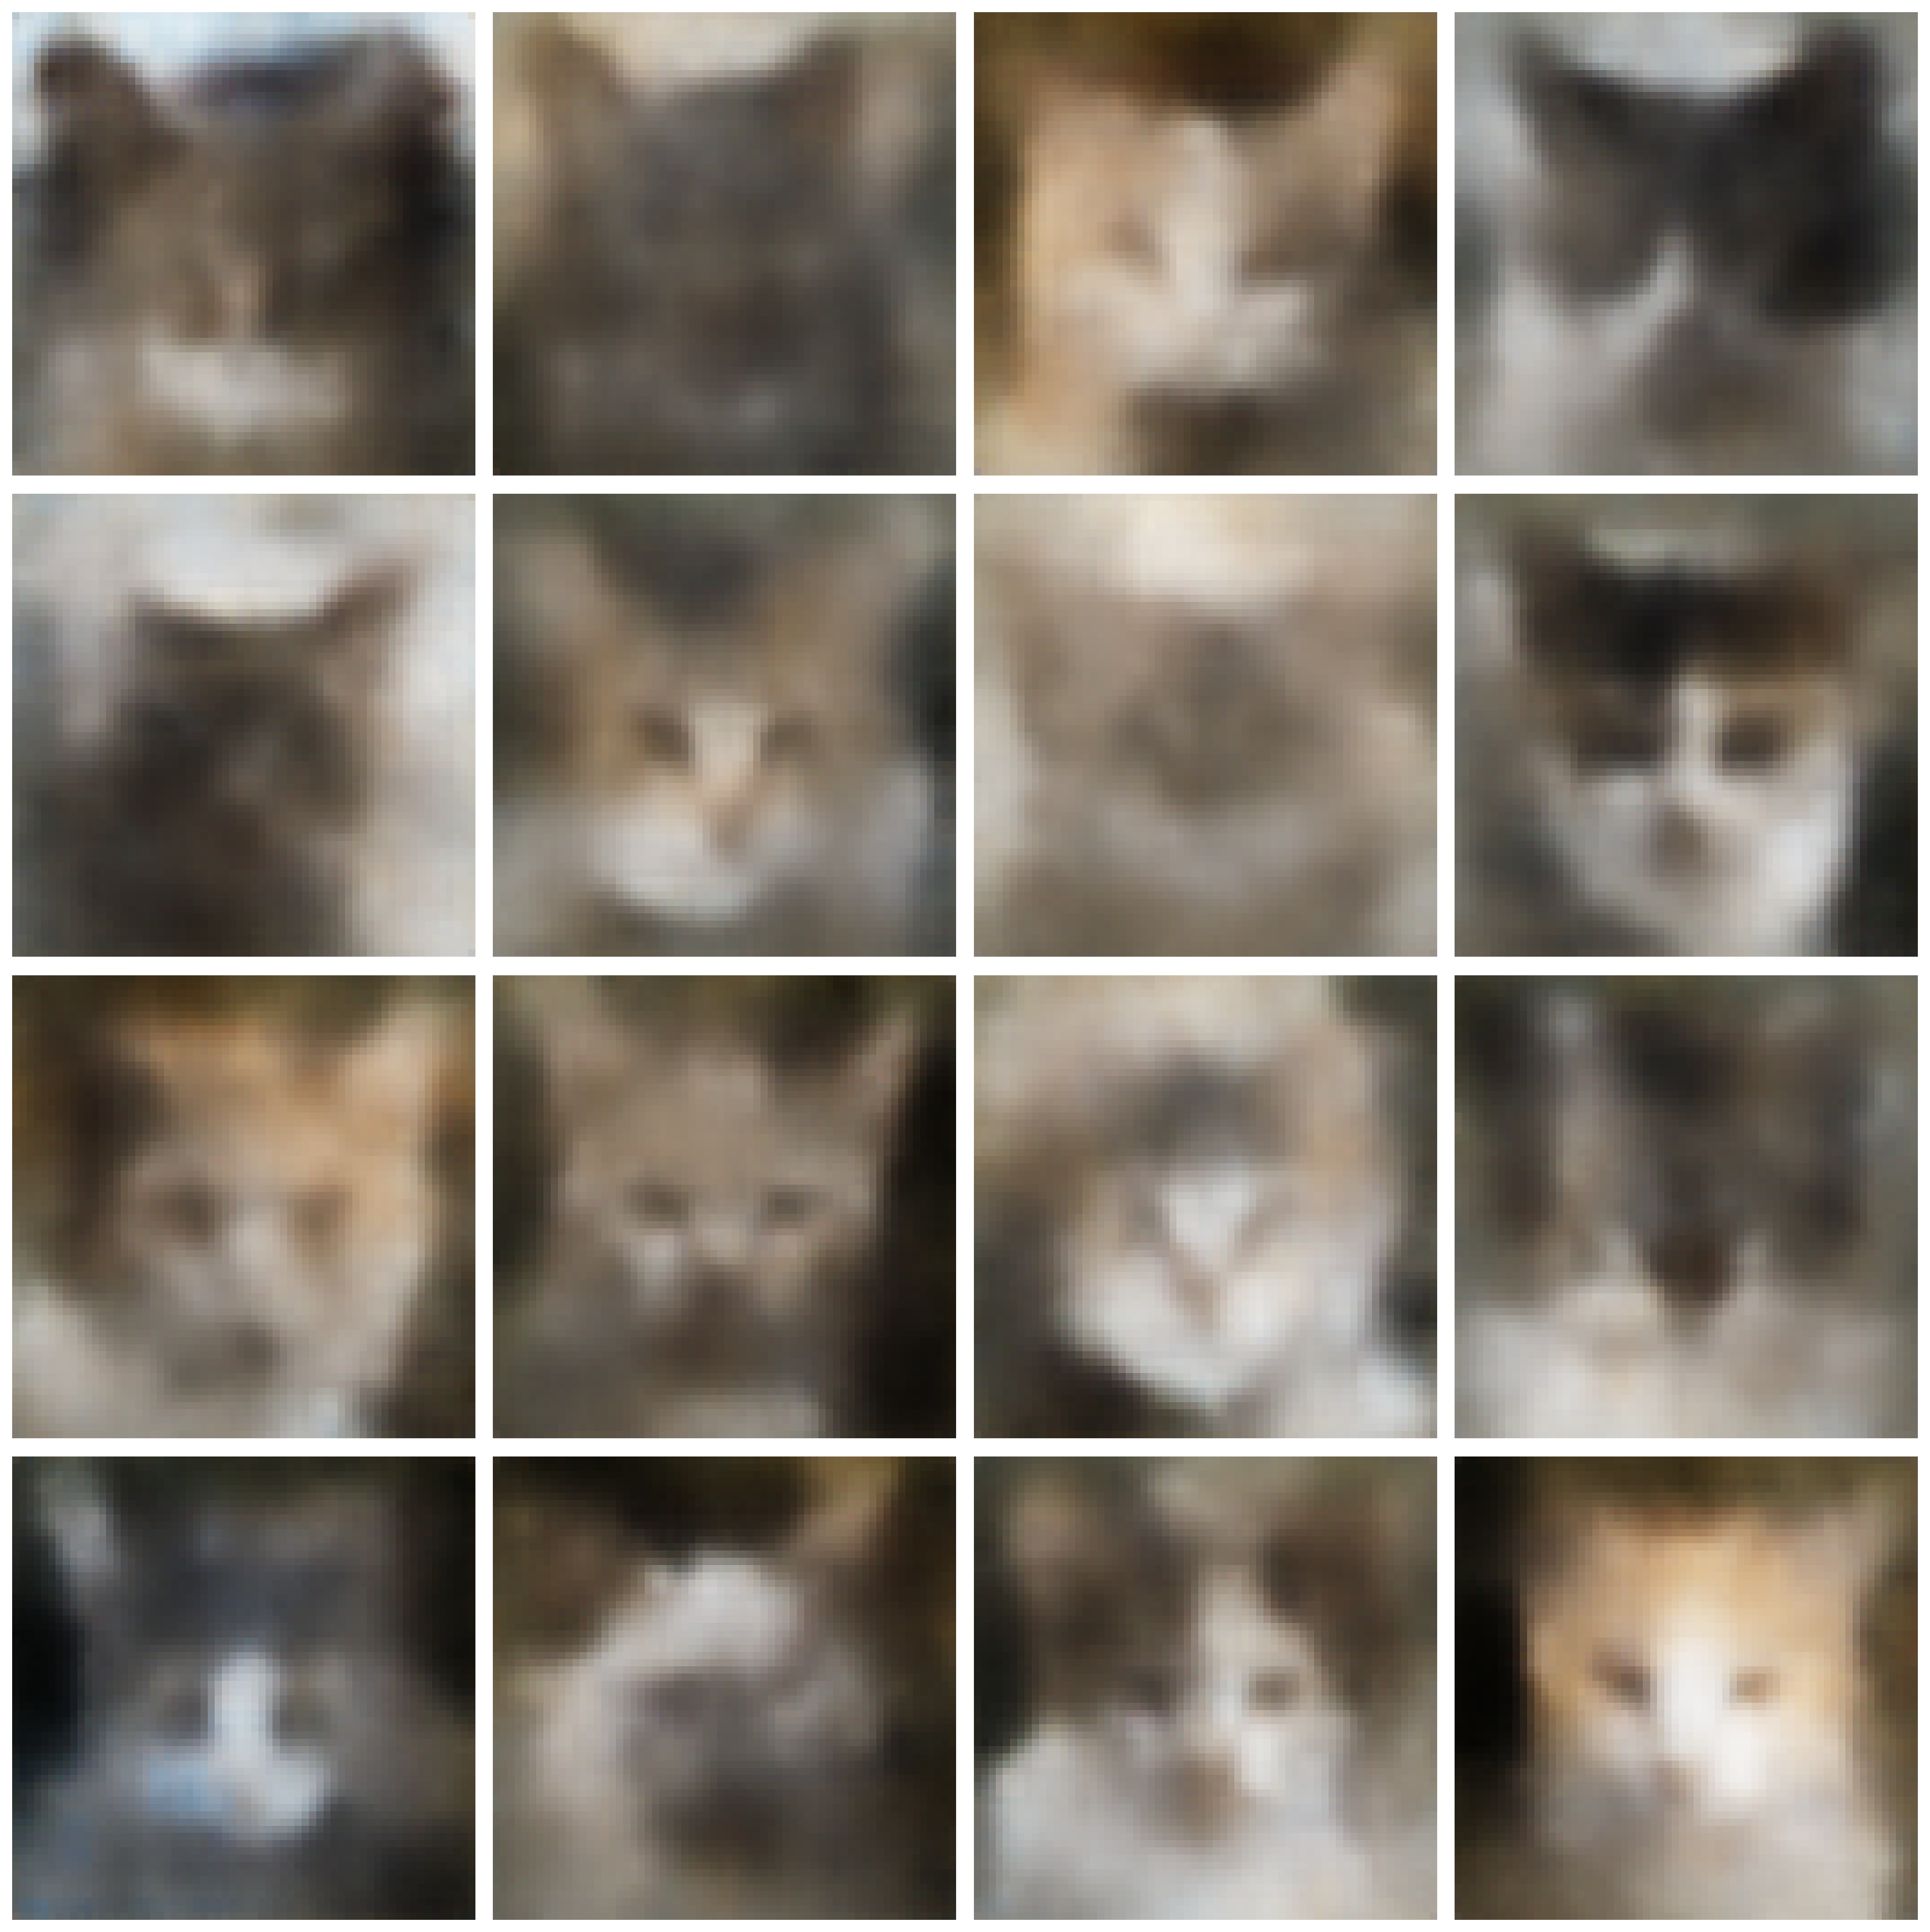
\includegraphics[width=0.5\linewidth]{vector_latent/VAE/generated_sample_x.png}
    \caption{Examples of generated images.}
    \label{fig:placeholder}
\end{figure}

\subsection{CNN VAE with a spatial latent representation}

\begin{figure}[H]
    \centering
    \begin{subfigure}{0.48\textwidth}
        \centering
         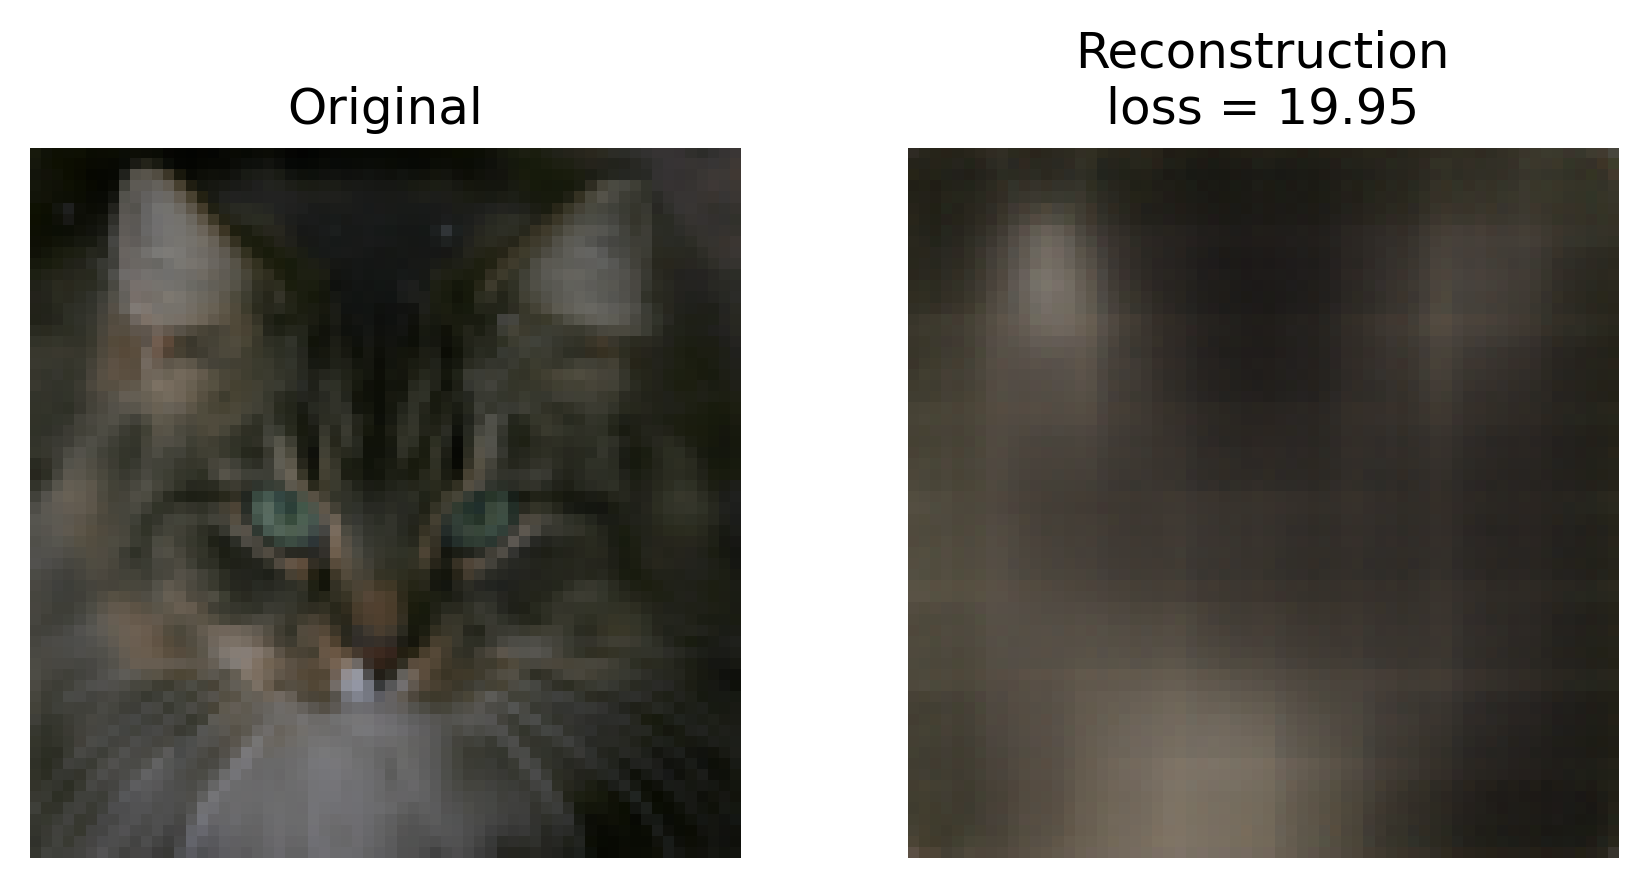
\includegraphics[width=\linewidth]{spatial_latent/VAE_spatial/train_best_2.png}
        \caption*{}
    \end{subfigure}
    \hspace{0.02\textwidth}
    \begin{subfigure}{0.48\textwidth}
        \centering
        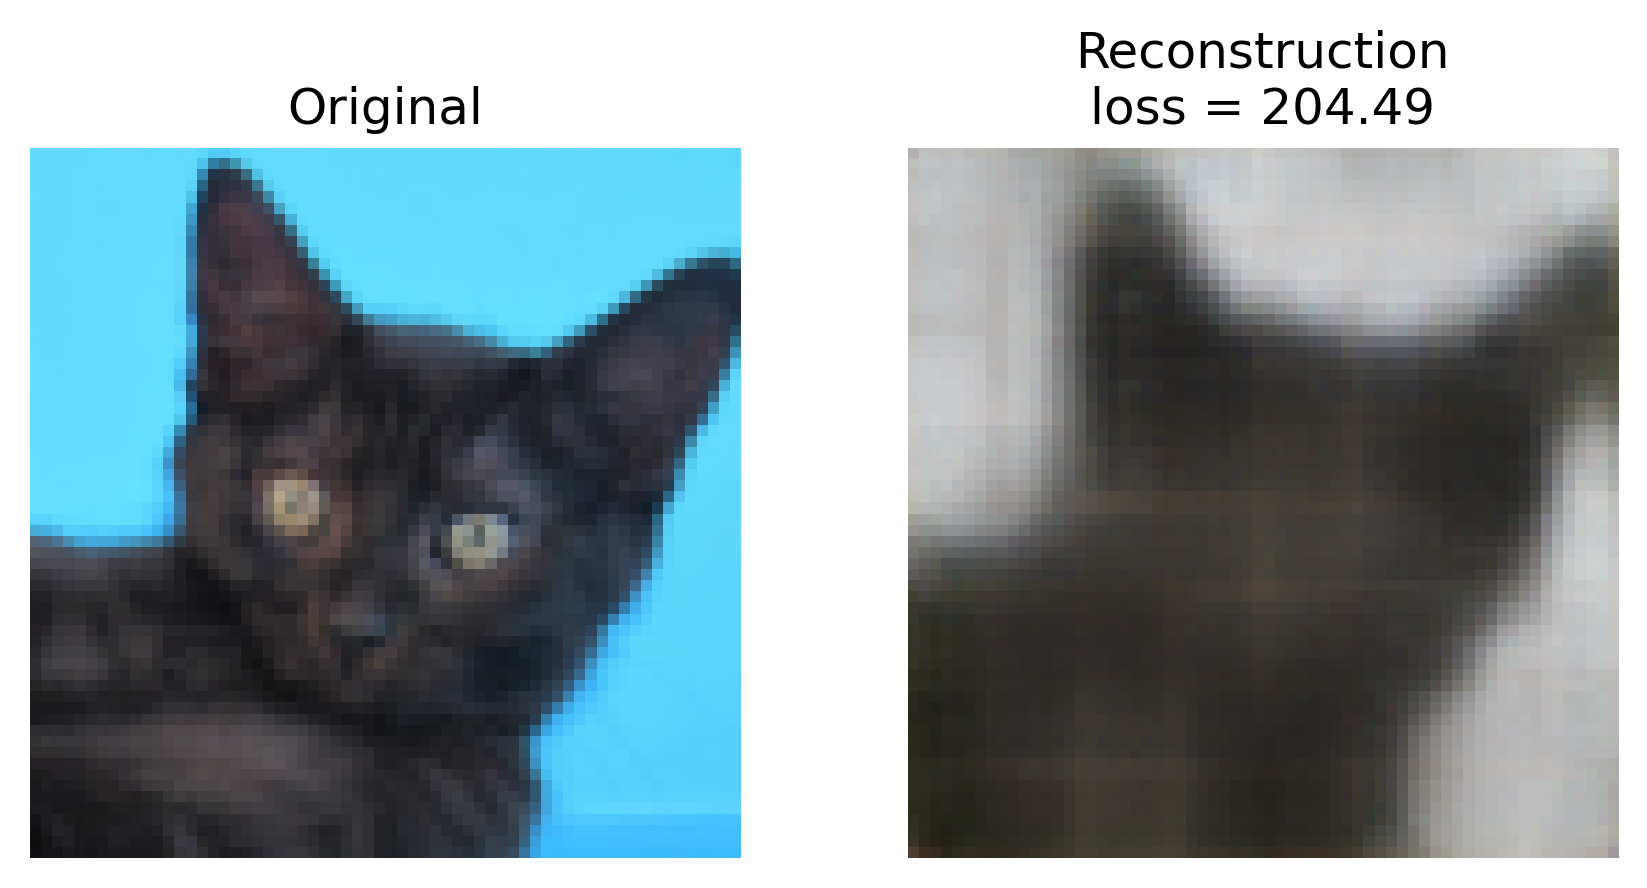
\includegraphics[width=\linewidth]{spatial_latent/VAE_spatial/val_worst_2.png}
        \caption*{}
    \end{subfigure}

    \caption{Examples of reconstruction quality for the spatial latent VAE.}
    \label{fig:spatial_latent_examples}
\end{figure}


\begin{figure}[H]
    \centering
    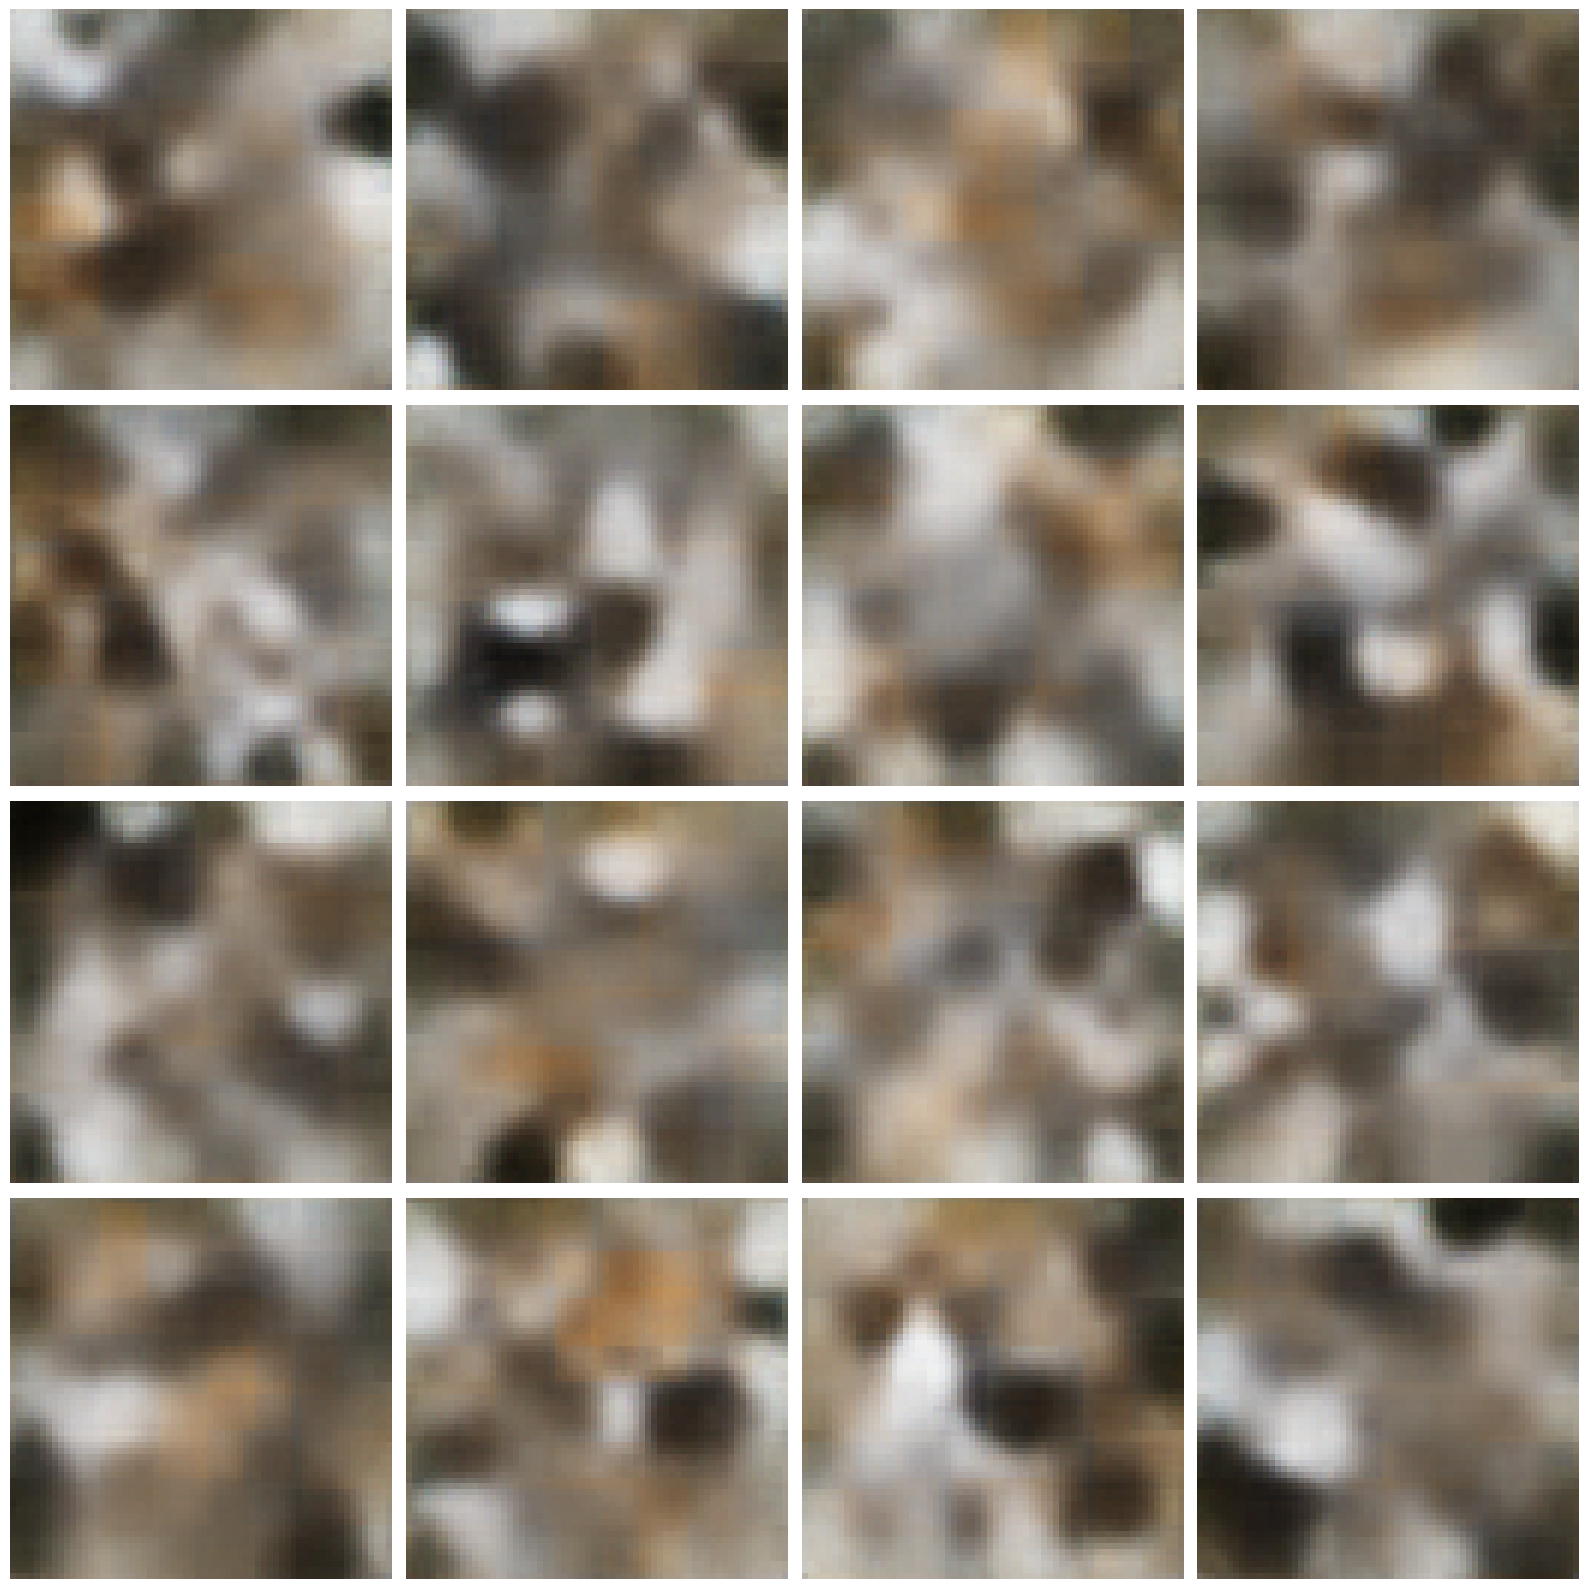
\includegraphics[width=0.5\linewidth]{spatial_latent/VAE_spatial/generated.png}
    \caption{Examples of generated images.}
    \label{fig:placeholder}
\end{figure}

\section{Experiments}
\subsection{Influence of Latent Dimensionality with $\beta = 1$}

The following latent dimensions were tested:

\[
d_z \in \{32,64,128,256\}
\]

using standard KL regularization with $\beta=1$.

Increasing the nominal size of the latent space produced almost no substantial improvement in reconstruction or prior generation quality.

The KL-per-dimension analysis showed that many additional dimensions in larger latent spaces had values close to

\[
D_{\mathrm{KL},j} \approx 0.
\]


\begin{figure}[H]
    \centering
    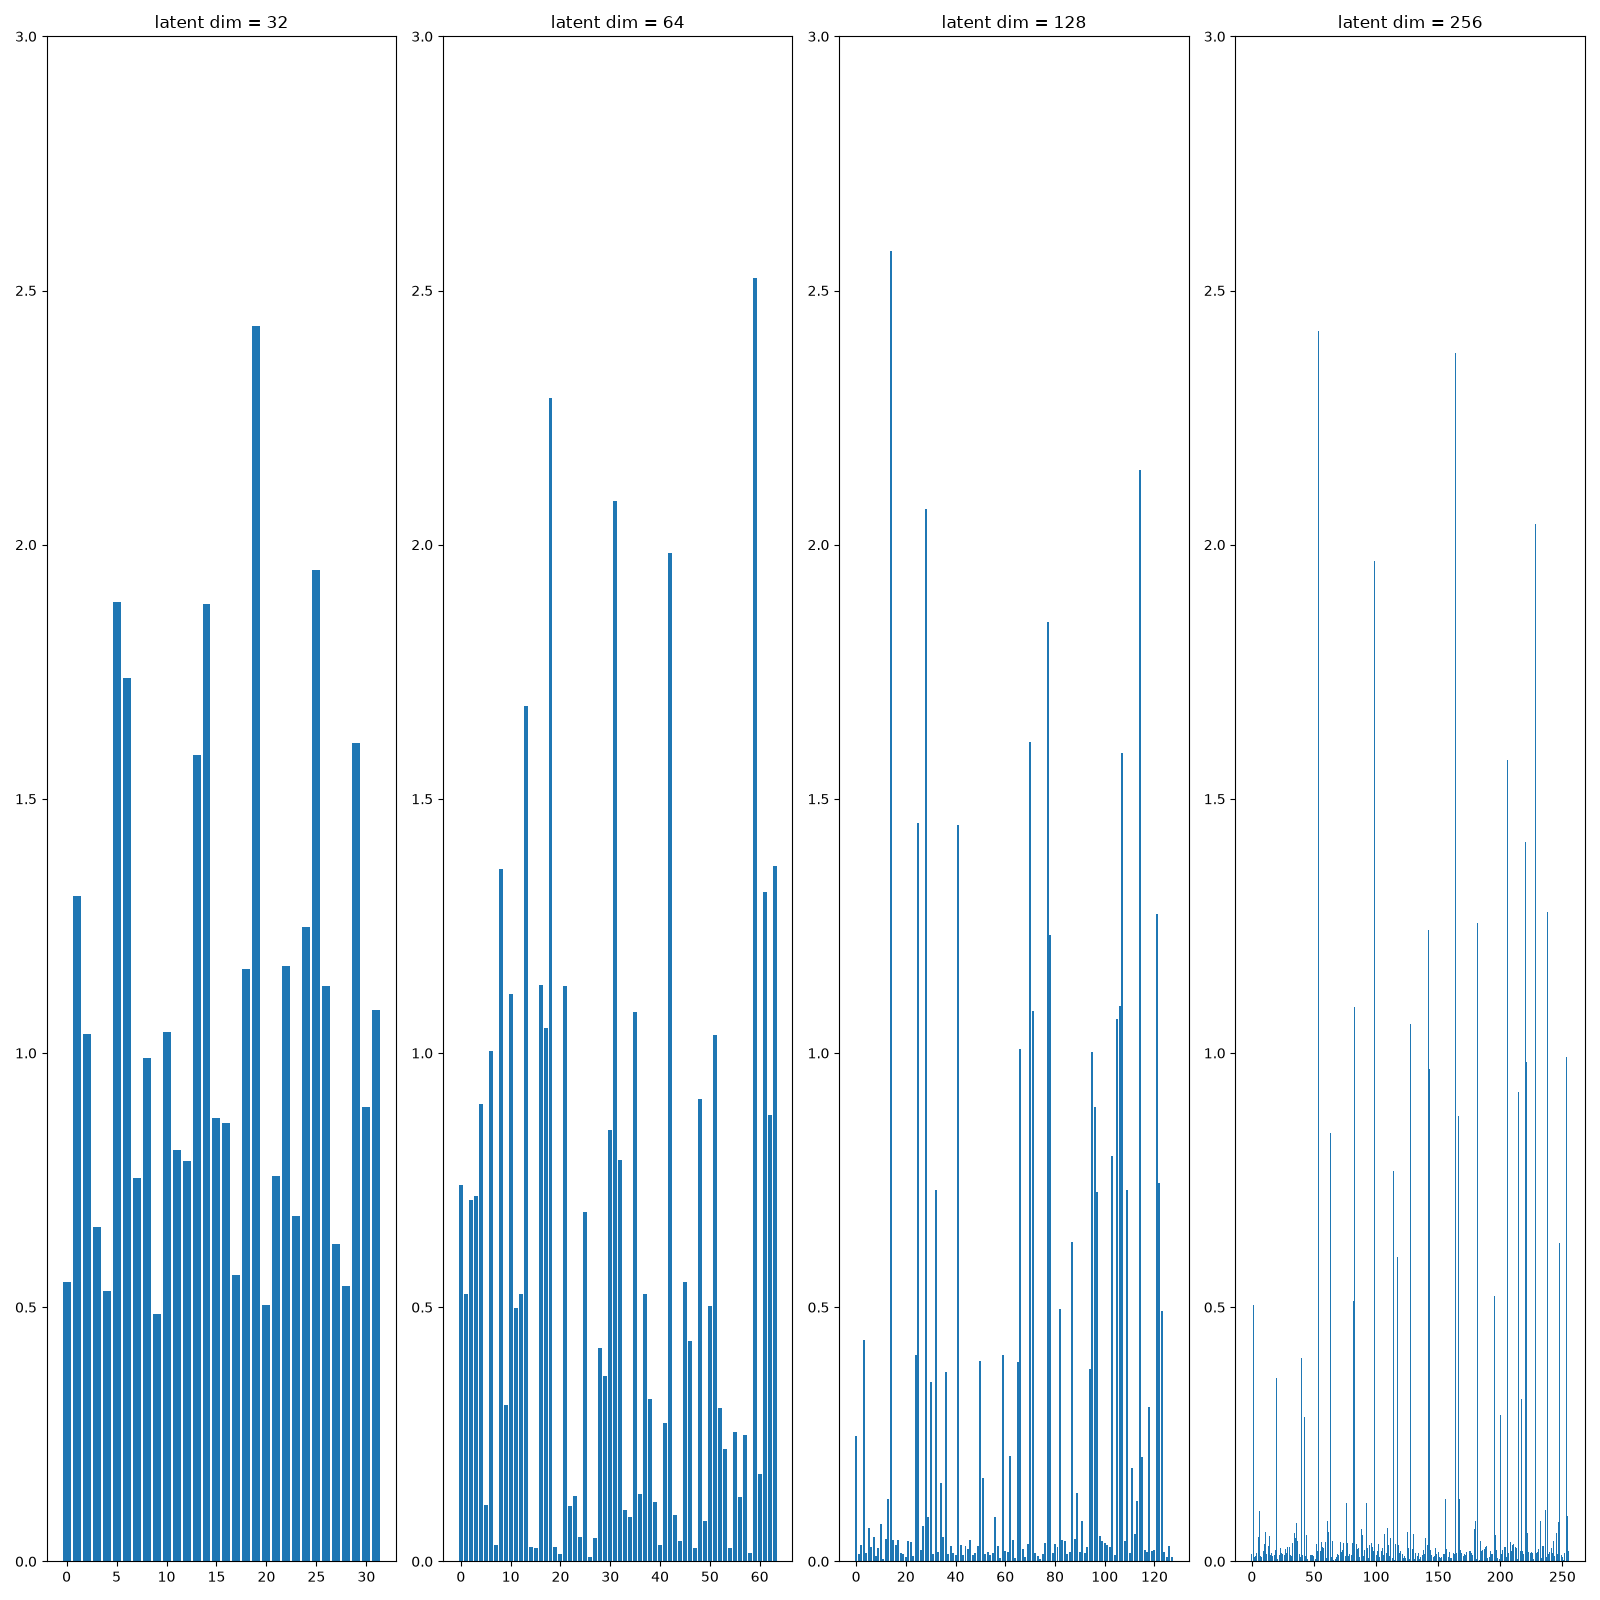
\includegraphics[width=0.75\linewidth]{vector_latent/kl_per_dimension_visualization.png}
    \caption{Enter Caption}
    \label{fig:placeholder}
\end{figure}


This indicates that these dimensions remained close to the prior distribution and carried little image-specific information.

\textbf{Conclusion:} increasing the nominal latent dimensionality does not necessarily increase the effective information capacity of the model. KL regularization can cause many additional latent dimensions to remain almost inactive.


\subsection{Experiments with Different Values of $\beta$}

For a latent dimension of

\[
d_z = 64,
\]

several values of the KL weight were tested:

\[
\beta \in \{0,0.1,0.5,1,2\}.
\]

The qualitative results are summarized in Table~\ref{tab:beta_comparison}.

\begin{table}[h]
\centering
\renewcommand{\arraystretch}{1.25}
\begin{tabular}{c|c|c}
\hline
$\beta$
& Reconstruction
& Prior generation \\
\hline
0
& Best
& Very poor \\

0.1
& Good
& Poor \\

0.5
& Good
& Reasonable \\

1
& More blurred
& Reasonable \\

2
& More blurred
& Similar to $\beta=1$ \\
\hline
\end{tabular}
\caption{Qualitative influence of the KL weight for a CNN VAE with $d_z=64$.}
\label{tab:beta_comparison}
\end{table}

The main observations were:

\begin{itemize}
    \item \textbf{$\beta=0$:} reconstruction quality was the best, but samples generated from
    \[
    z \sim \mathcal{N}(0,I)
    \]
    were very poor. Without KL regularization, the encoded latent distribution was not sufficiently aligned with the prior.

    \item \textbf{$\beta=0.1$:} reconstruction quality remained good, but prior generation was still unreliable. The regularization was too weak to produce a latent space suitable for consistent random sampling.

    \item \textbf{$\beta=0.5$:} prior generation improved substantially and generated images became recognizable as cats, while reconstruction quality remained relatively good.

    \item \textbf{$\beta=1$:} prior generation remained reasonable, but reconstructions became more blurred. The stronger KL term reduced the amount of image-specific information that could be stored in the latent representation.

    \item \textbf{$\beta=2$:} reconstruction quality degraded further, while prior generation showed little visible improvement compared with $\beta=1$.
\end{itemize}

The experiment demonstrated a clear trade-off between reconstruction quality and the ability to generate meaningful images from the prior.

\textbf{Conclusion:} KL regularization is necessary for meaningful prior sampling, but increasing its strength also limits the amount of information that can be stored in the latent representation. In the tested configuration, $\beta \approx 0.5$ provided a useful compromise between reconstruction quality and prior generation.


\subsection{Exploration of a Two-Dimensional Latent Space}

A separate experiment was performed using a two-dimensional latent representation:

\[
d_z = 2.
\]

The main goal of this experiment was not to maximize reconstruction quality, but to make the latent space directly visualizable and to observe how KL regularization changes its structure.

For each image, the posterior mean

\[
\mu = (\mu_1,\mu_2)
\]

was plotted as a point in the two-dimensional latent space.

Several values of $\beta$ were compared in order to observe how strongly the latent distribution was constrained toward the standard normal prior.

\begin{figure}[H]
    \centering
    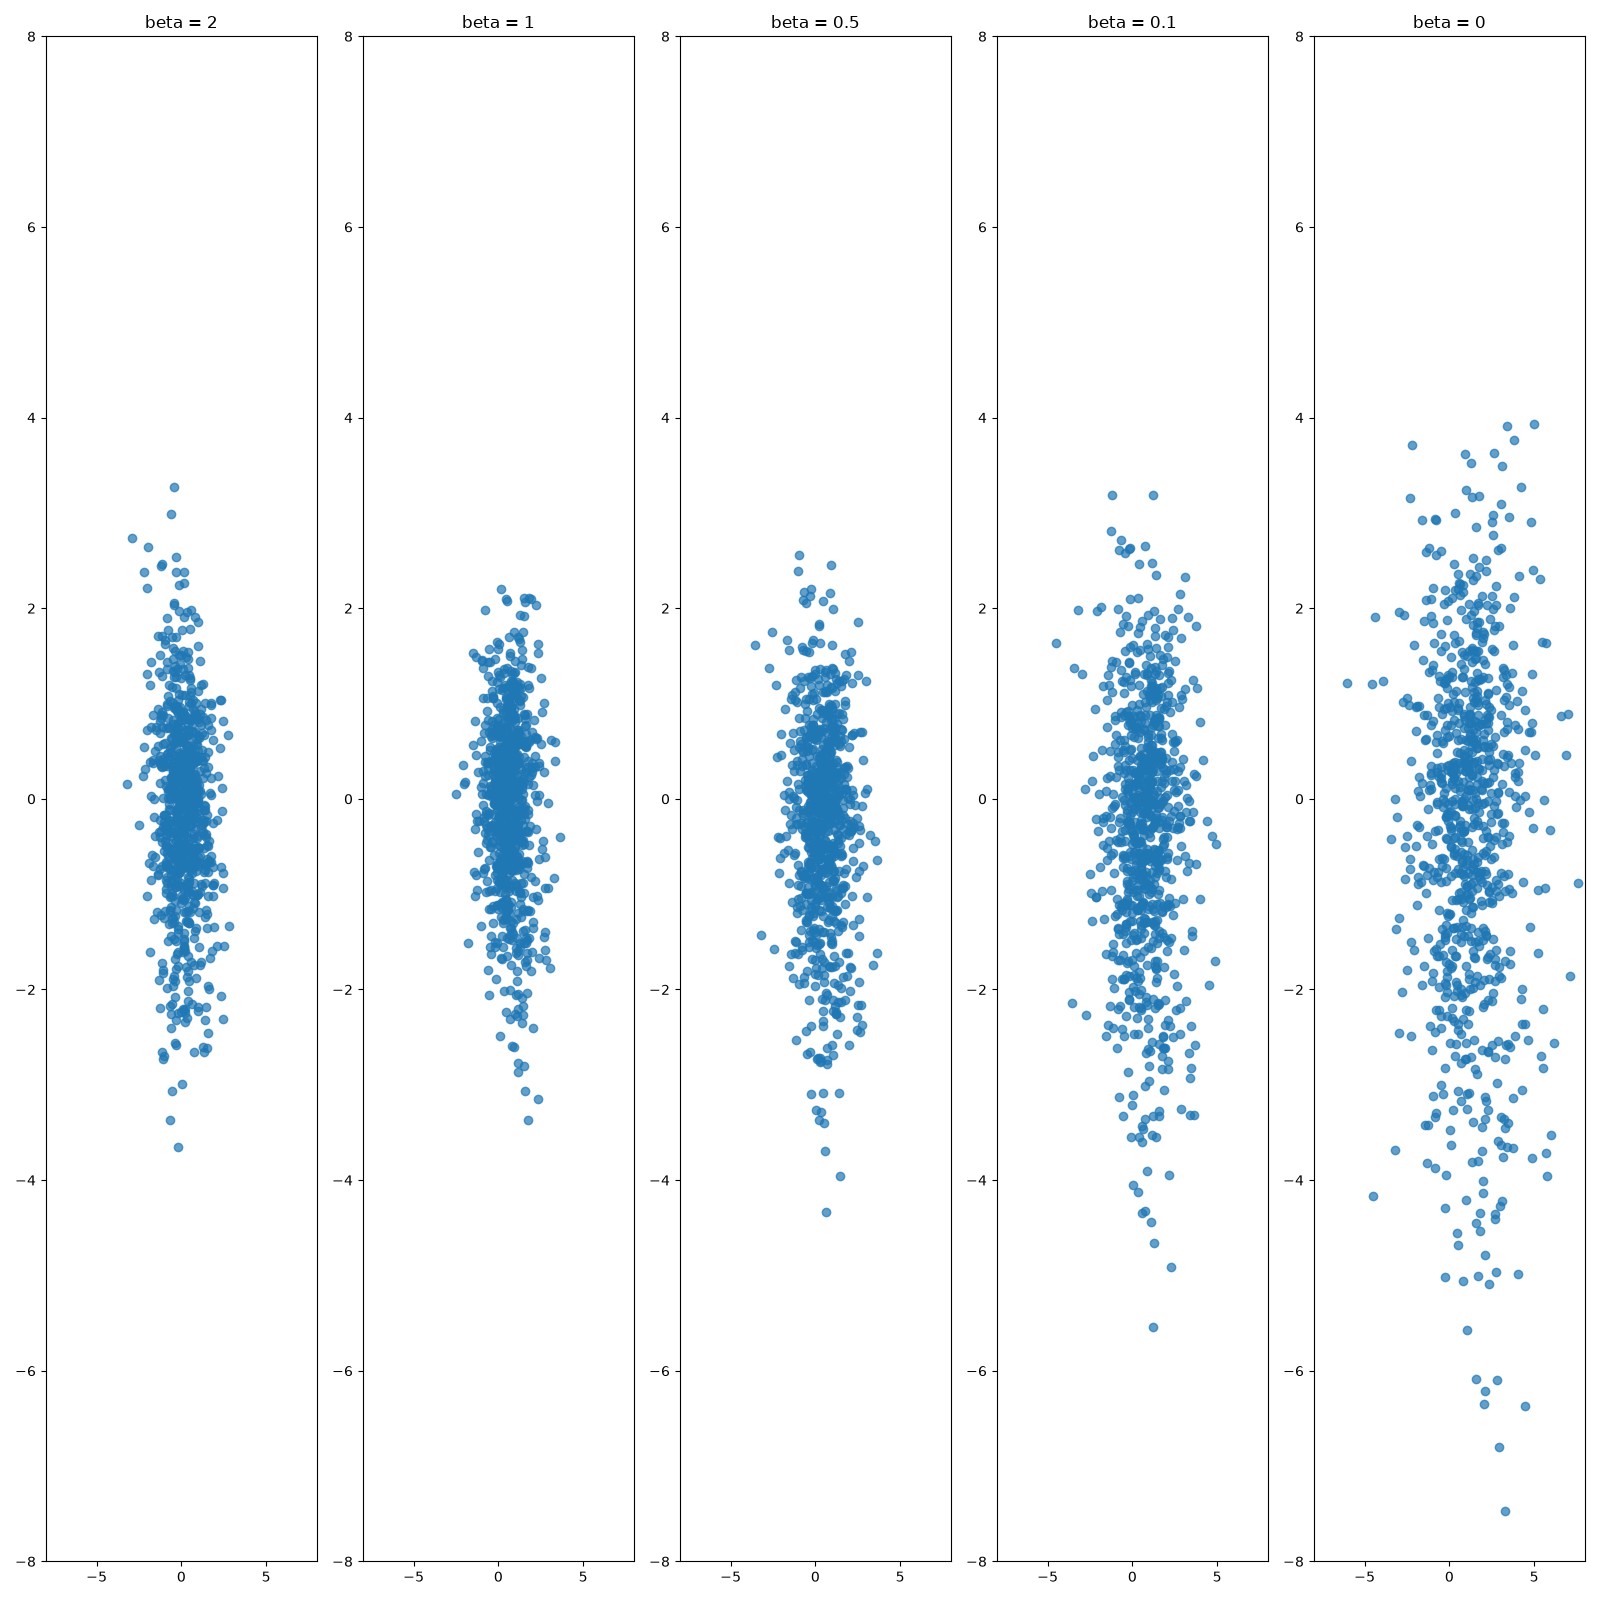
\includegraphics[width=0.5\linewidth]{vector_latent/latent2_visualization.png}
    \caption{Visualization of the two-dimensional latent space for different values of $\beta$.}
    \label{fig:latent2_visualization}
\end{figure}

The following behaviour was observed:

\begin{itemize}
    \item for low values of $\beta$, the latent representations were more dispersed and less concentrated around the center,

    \item for $\beta=0$, the latent distribution was especially spread out and showed little correspondence with the standard normal prior,

    \item increasing $\beta$ caused the latent representations to become progressively more compact,

    \item for larger values of $\beta$, the encoded means were more strongly concentrated around the central region of the latent space.
\end{itemize}

The experiment visually demonstrated the effect of KL regularization on the geometry of the latent representation.

Lower KL pressure allows the encoder to place different images more freely in latent space, which can improve reconstruction but leads to poor compatibility with the prior.

Stronger KL regularization reduces this freedom and makes the latent representation more similar to the target distribution

\[
\mathcal{N}(0,I).
\]

\textbf{Conclusion:} the two-dimensional latent-space experiment provided a direct visual confirmation of the trade-off observed in the $\beta$ experiments. Lower values of $\beta$ allow more flexible image encoding, while higher values organize the latent space more strongly around the prior distribution.


\subsection{KL Annealing}

KL annealing was tested in order to allow the model to focus more strongly on reconstruction during the early stage of training.

Instead of applying the full KL regularization immediately, the KL weight was increased linearly during the first 15 epochs:

\[
\beta_t
=
\min\left(
1,
\frac{t+1}{15}
\right).
\]

After epoch 15, the standard value $\beta=1$ was used for the remainder of training.

During the annealing period, the model achieved lower reconstruction loss and higher raw KL divergence than the model trained with the full KL penalty from the beginning. This indicates that the encoder initially used more latent information when the KL constraint was weaker.

However, once the KL weight reached its final value, the results gradually approached those obtained with standard training. No clear final improvement in reconstruction sharpness was observed.

\textbf{Conclusion:} KL annealing changed the early training dynamics and temporarily allowed the model to use more latent information, but it did not provide a substantial final reduction in reconstruction blur.


\section{Experiments Investigating Reconstruction Blur}

\subsection{Reconstruction with and without Stochastic Sampling}

Reconstructions were compared using the standard stochastic latent representation

\[
z = \mu + \sigma\epsilon
\]

and a deterministic representation

\[
z = \mu.
\]

Removing the random variable $\epsilon$ did not substantially reduce reconstruction blur.

\begin{figure}[H]
    \centering

    \begin{subfigure}{0.48\textwidth}
        \centering
        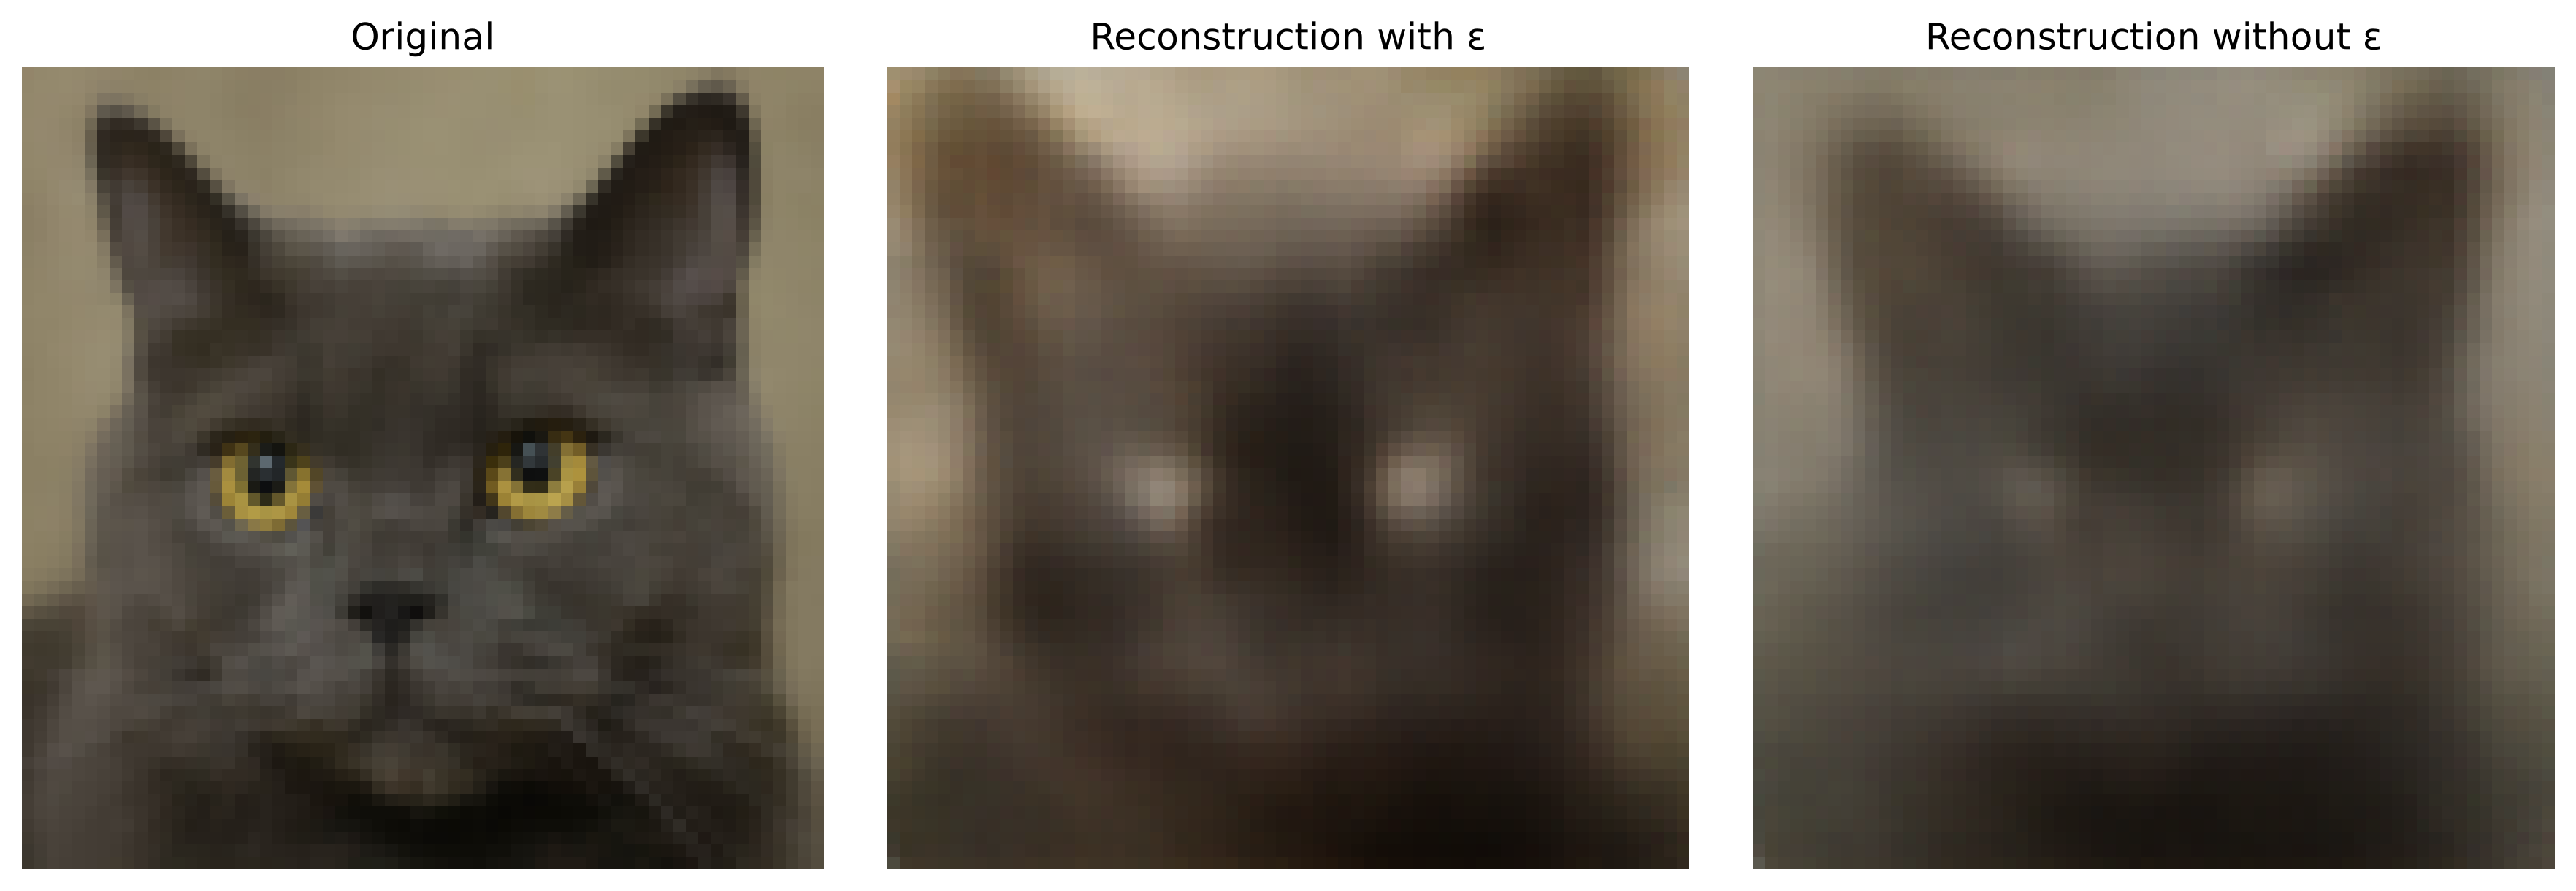
\includegraphics[width=\linewidth]{vector_latent/RQ2/reconstruction_without_epsilon/reconstruction_comparison_1.png}
        \caption*{}
    \end{subfigure}
    \hspace{0.02\textwidth}
    \begin{subfigure}{0.48\textwidth}
        \centering
        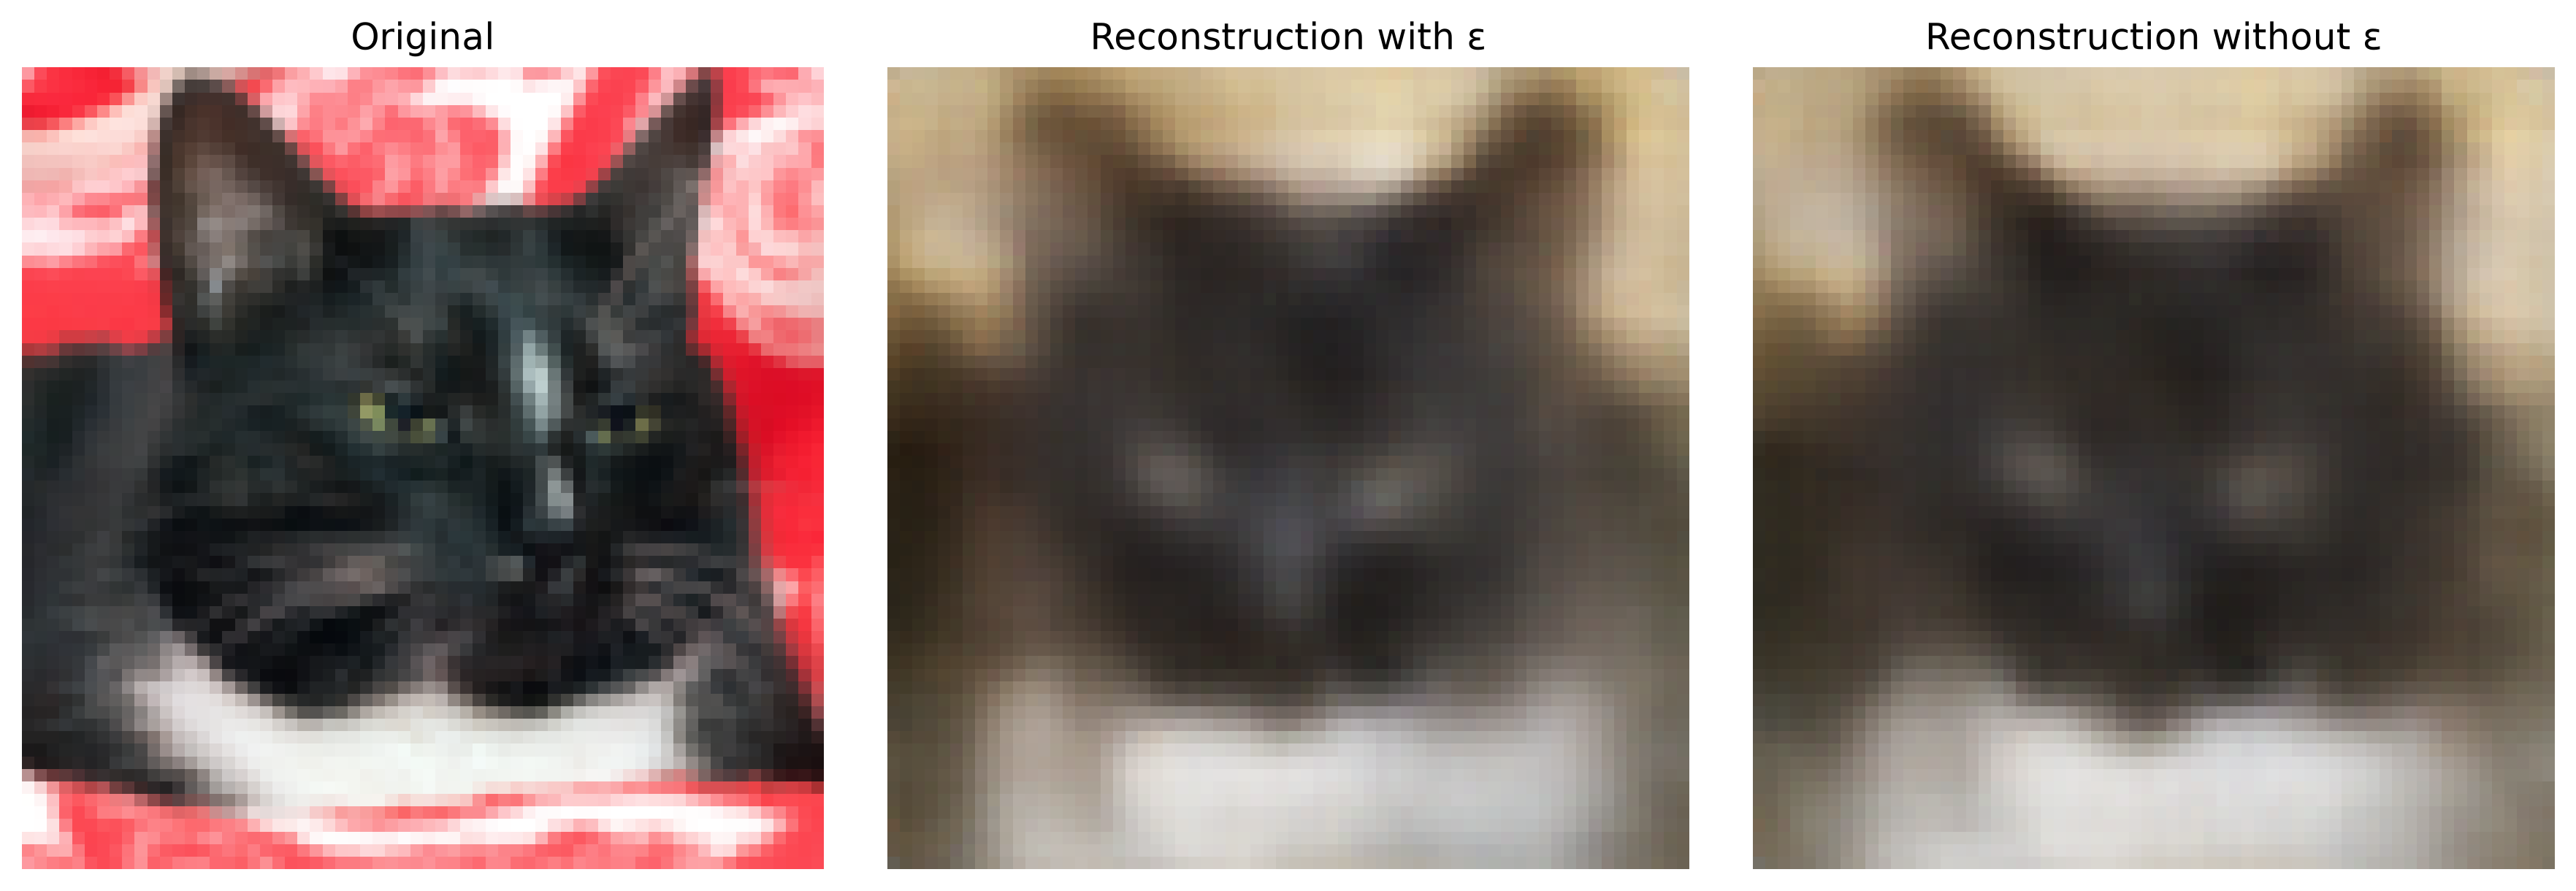
\includegraphics[width=\linewidth]{vector_latent/RQ2/reconstruction_without_epsilon/reconstruction_comparison_6.png}
        \caption*{}
    \end{subfigure}

    \caption{Examples of reconstruction quality for the spatial latent VAE stochastic.}
    \label{fig:spatial_latent_examples}
\end{figure}

In some cases, deterministic reconstruction improved the placement or consistency of certain facial features, but fine details remained blurred.

\textbf{Conclusion:} stochastic latent sampling is not the primary cause of reconstruction blur.


\subsection{Gaussian Reconstruction Loss vs. Laplace/L1 Loss}

The baseline reconstruction objective was based on a Gaussian likelihood:

\[
L_{\mathrm{rec}}
=
\frac{1}{2}
\sum_i
(x_i-\hat{x}_i)^2.
\]

This loss was compared with a Laplace/L1 reconstruction objective.

For a Laplace scale of $b=1$, the approximate loss values were

\[
L_{\mathrm{rec}} \approx 900,
\qquad
D_{\mathrm{KL}} \approx 100.
\]

The reconstructions appeared slightly sharper, but the quality of prior generation became very poor.

\begin{figure}[H]
    \centering

    \begin{subfigure}{0.48\textwidth}
        \centering
        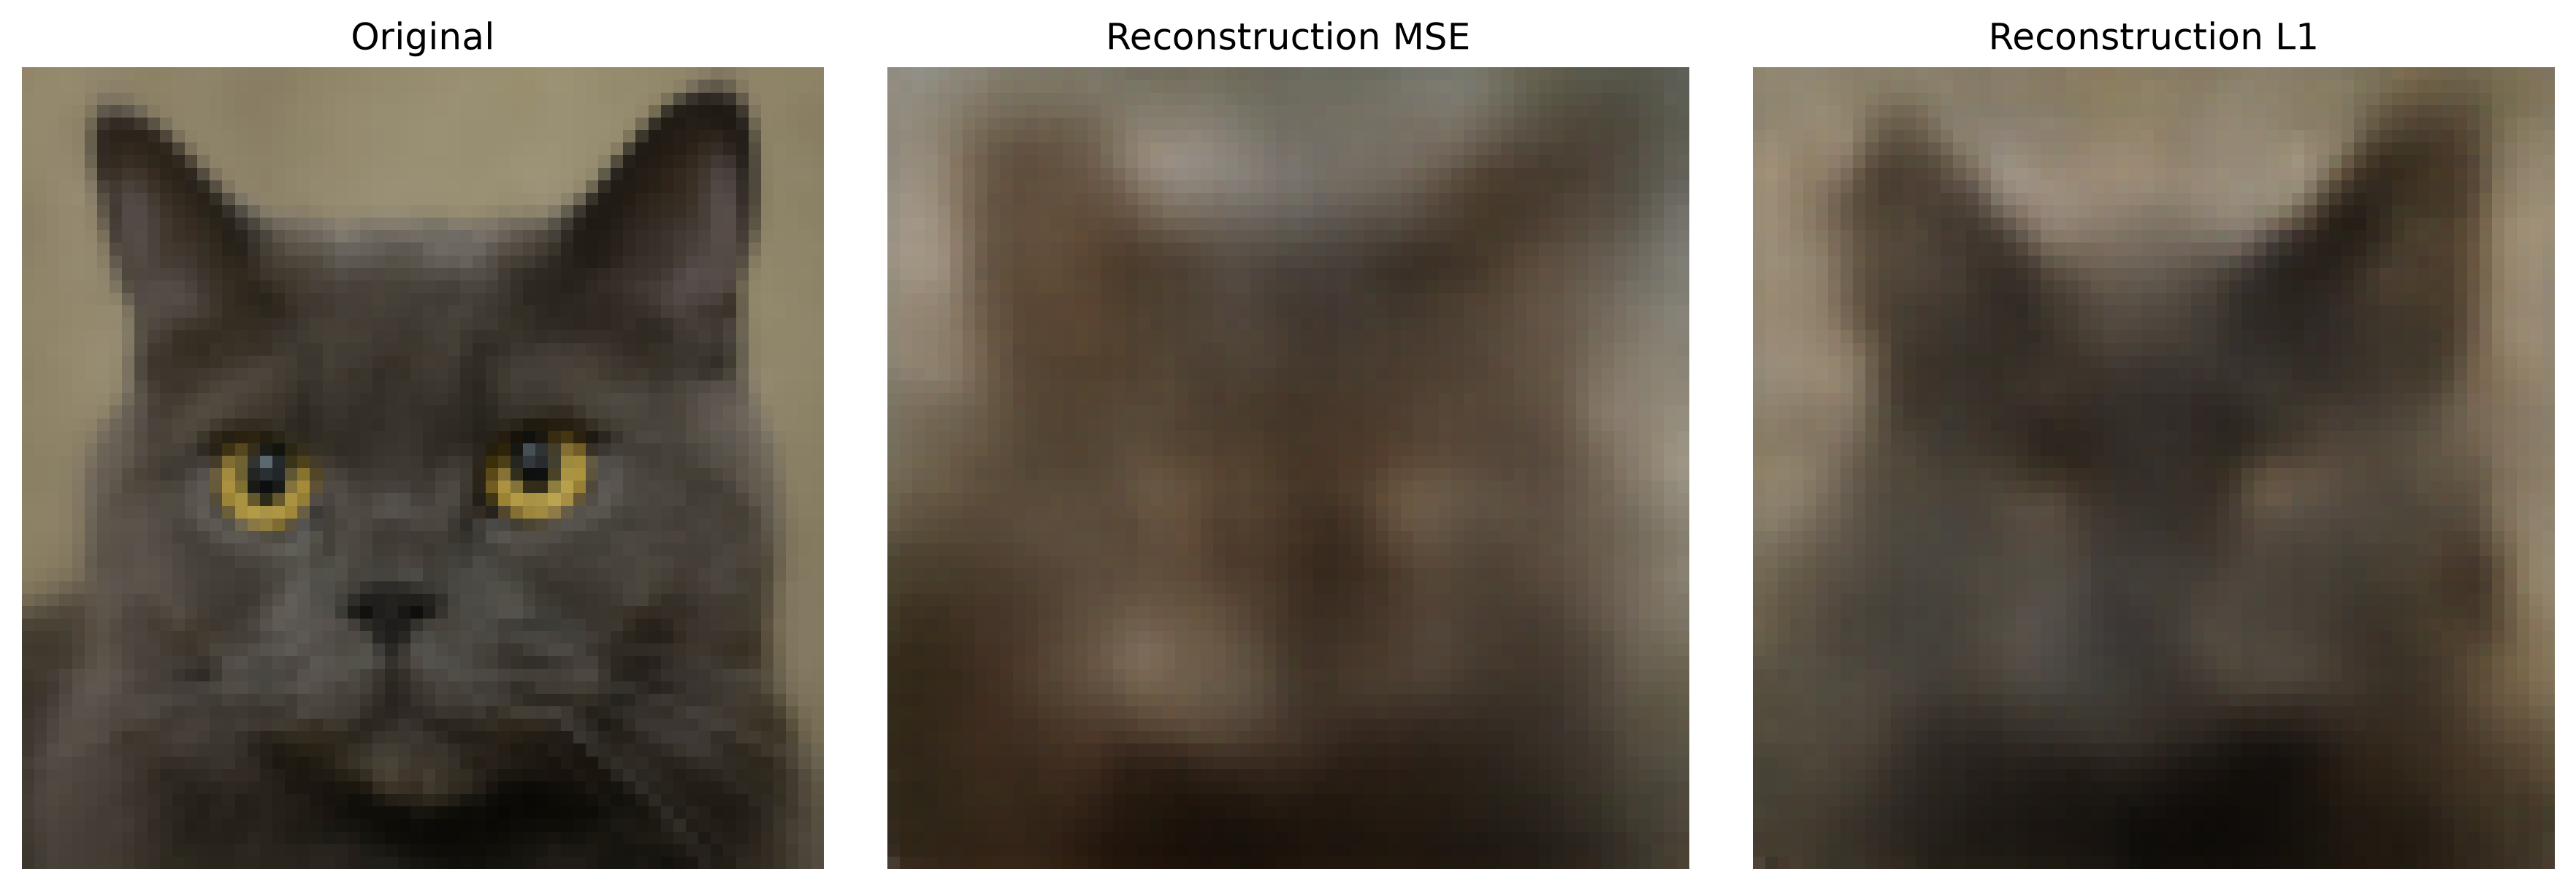
\includegraphics[width=\linewidth]{vector_latent/RQ2/L1/L1_b1/reconstruction_comparison_1.png}
        \caption*{}
    \end{subfigure}
    \hspace{0.02\textwidth}
    \begin{subfigure}{0.48\textwidth}
        \centering
        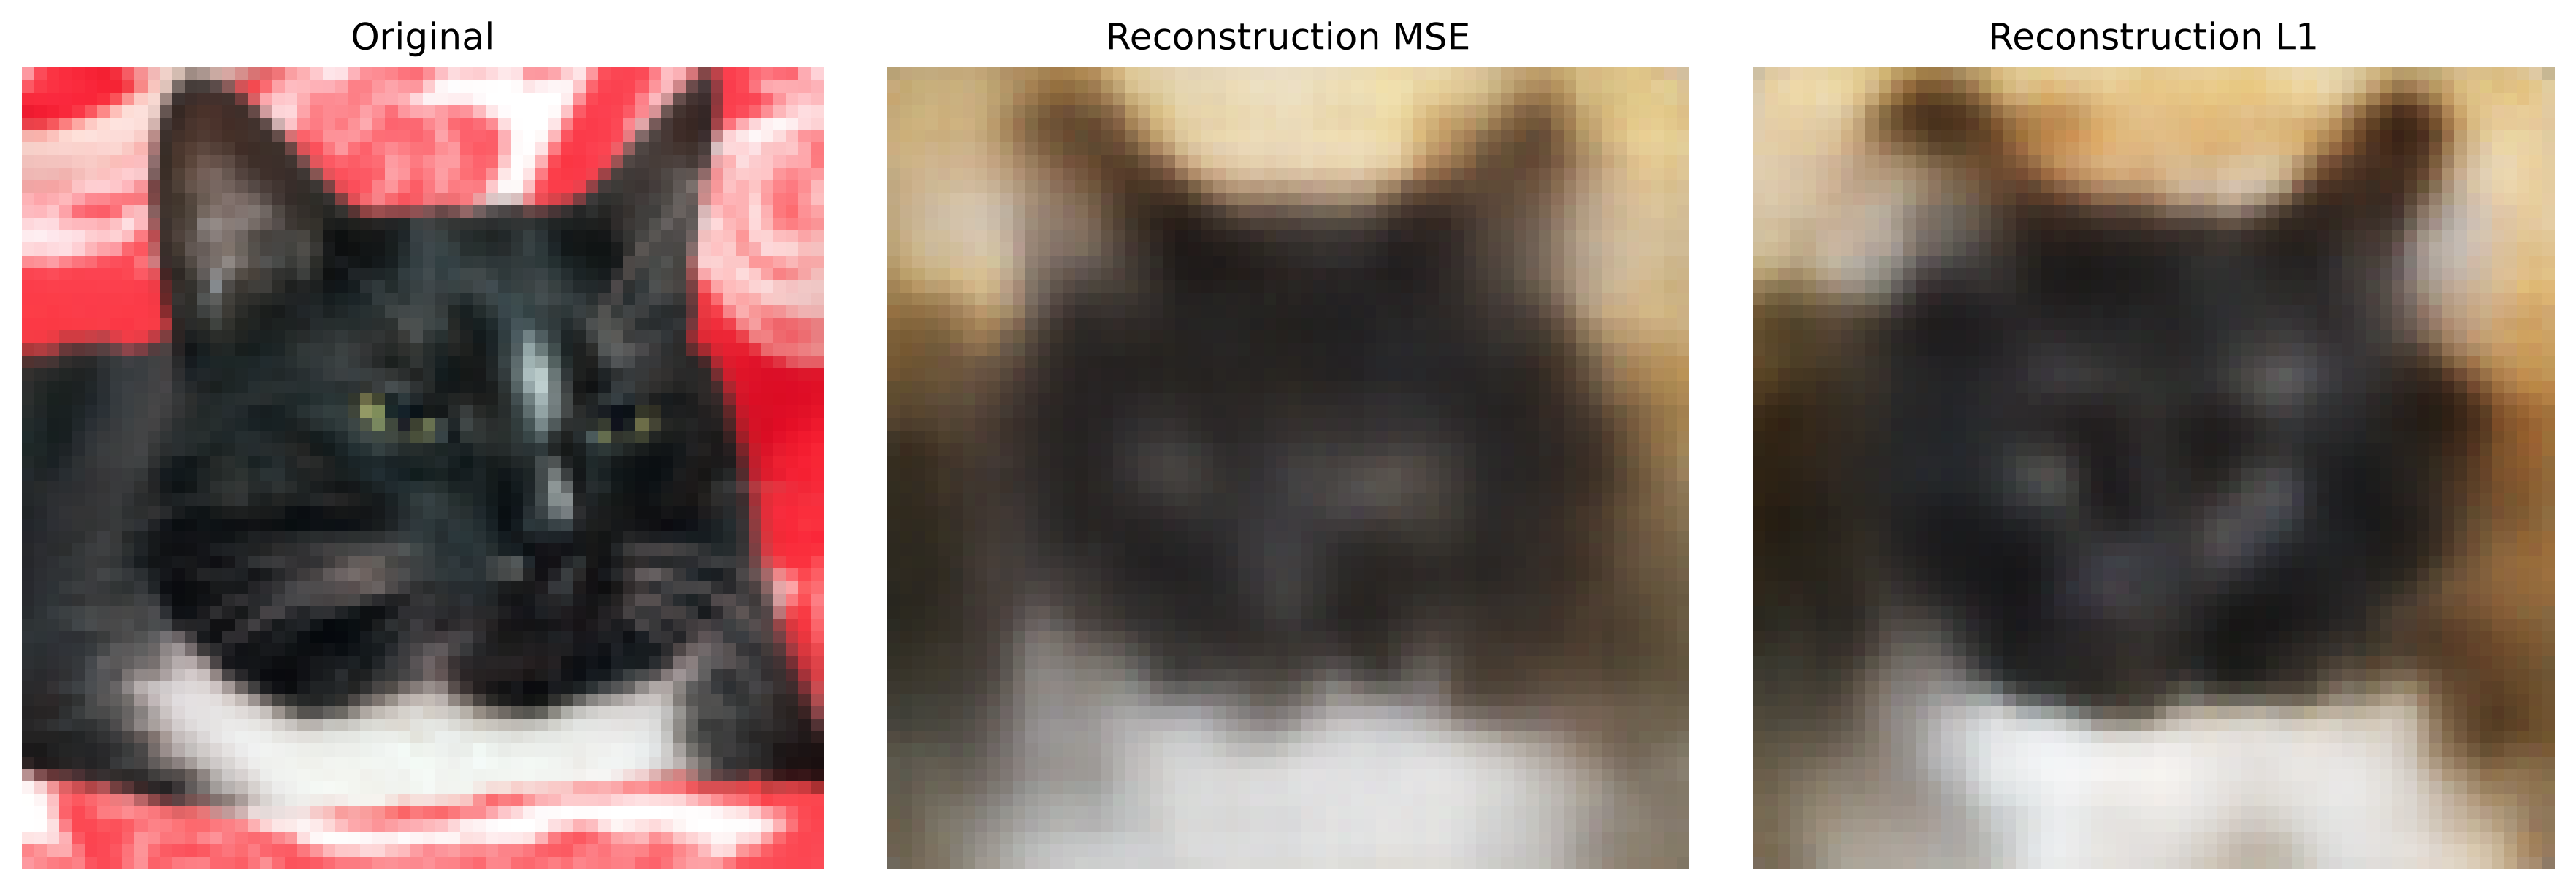
\includegraphics[width=\linewidth]{vector_latent/RQ2/L1/L1_b1/reconstruction_comparison_6.png}
        \caption*{}
    \end{subfigure}

    \caption{Examples of reconstruction quality for the spatial latent VAE stochastic.}
    \label{fig:generated l1}
\end{figure}

\begin{figure}[H]
    \centering
    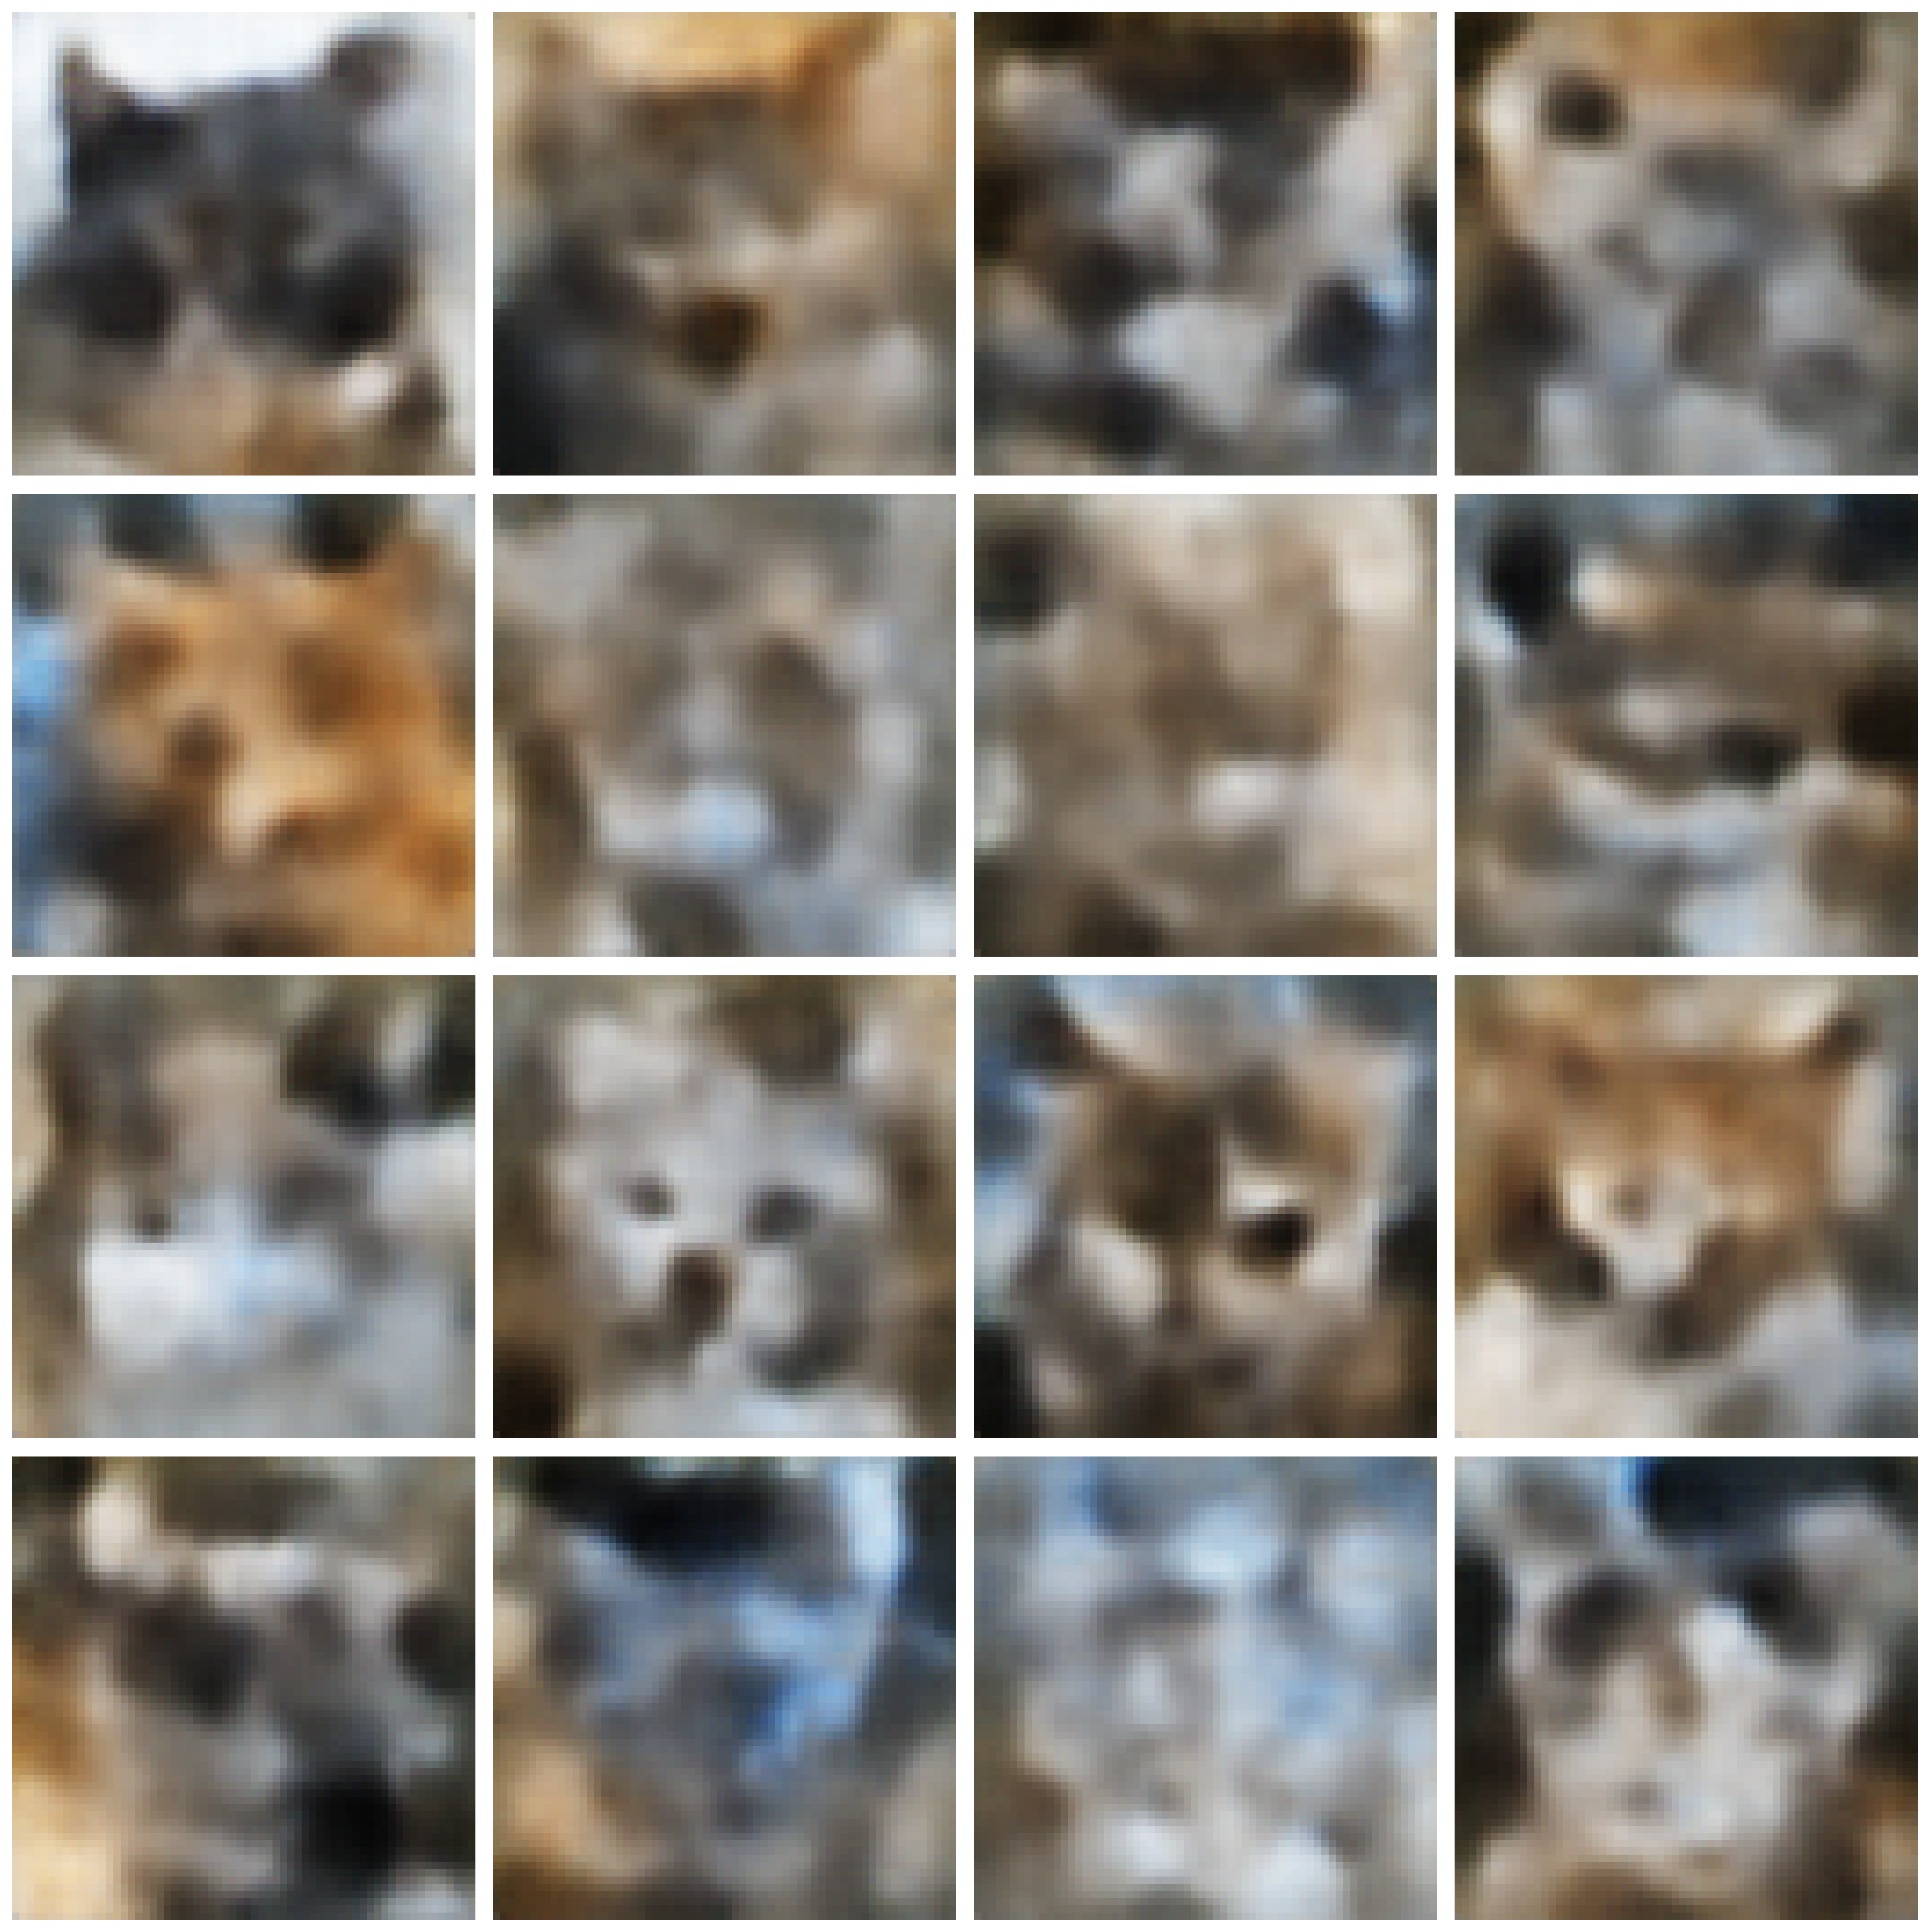
\includegraphics[width=0.4\linewidth]{vector_latent/RQ2/L1/L1_b1/generated_sample_x.png}
    \caption{Generated images.}
    \label{fig:placeholder}
\end{figure}

The Laplace scale was then changed to $b=9$ in order to make the magnitude of the reconstruction term more comparable with the Gaussian baseline. The approximate values became

\[
L_{\mathrm{rec}} \approx 100,
\qquad
D_{\mathrm{KL}} \approx 30.
\]

After making the loss scales more comparable, the apparent advantage of the L1 reconstruction objective mostly disappeared.

\begin{figure}[H]
    \centering

    \begin{subfigure}{0.48\textwidth}
        \centering
        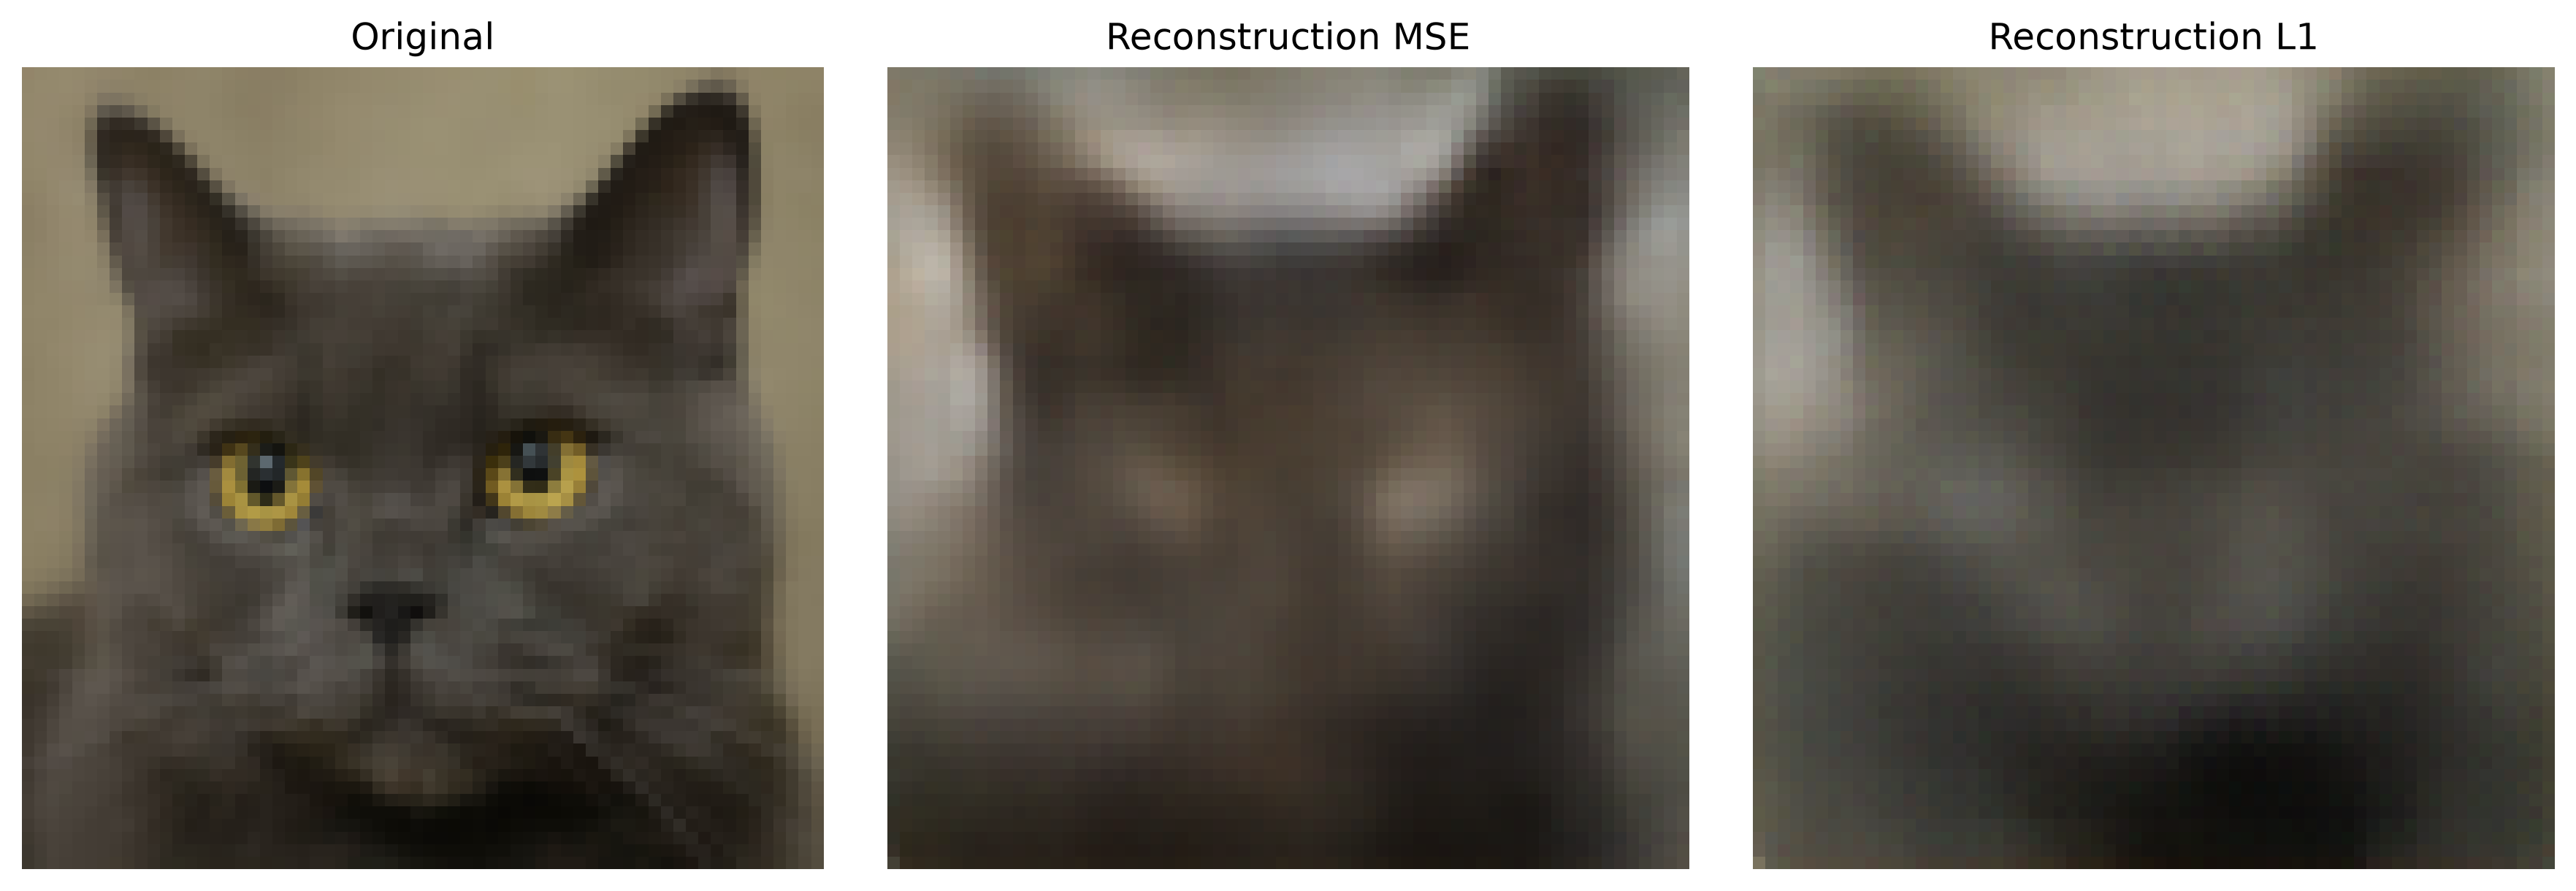
\includegraphics[width=\linewidth]{vector_latent/RQ2/L1/L1_b9/reconstruction_comparison_1.png}
        \caption*{}
    \end{subfigure}
    \hspace{0.02\textwidth}
    \begin{subfigure}{0.48\textwidth}
        \centering
        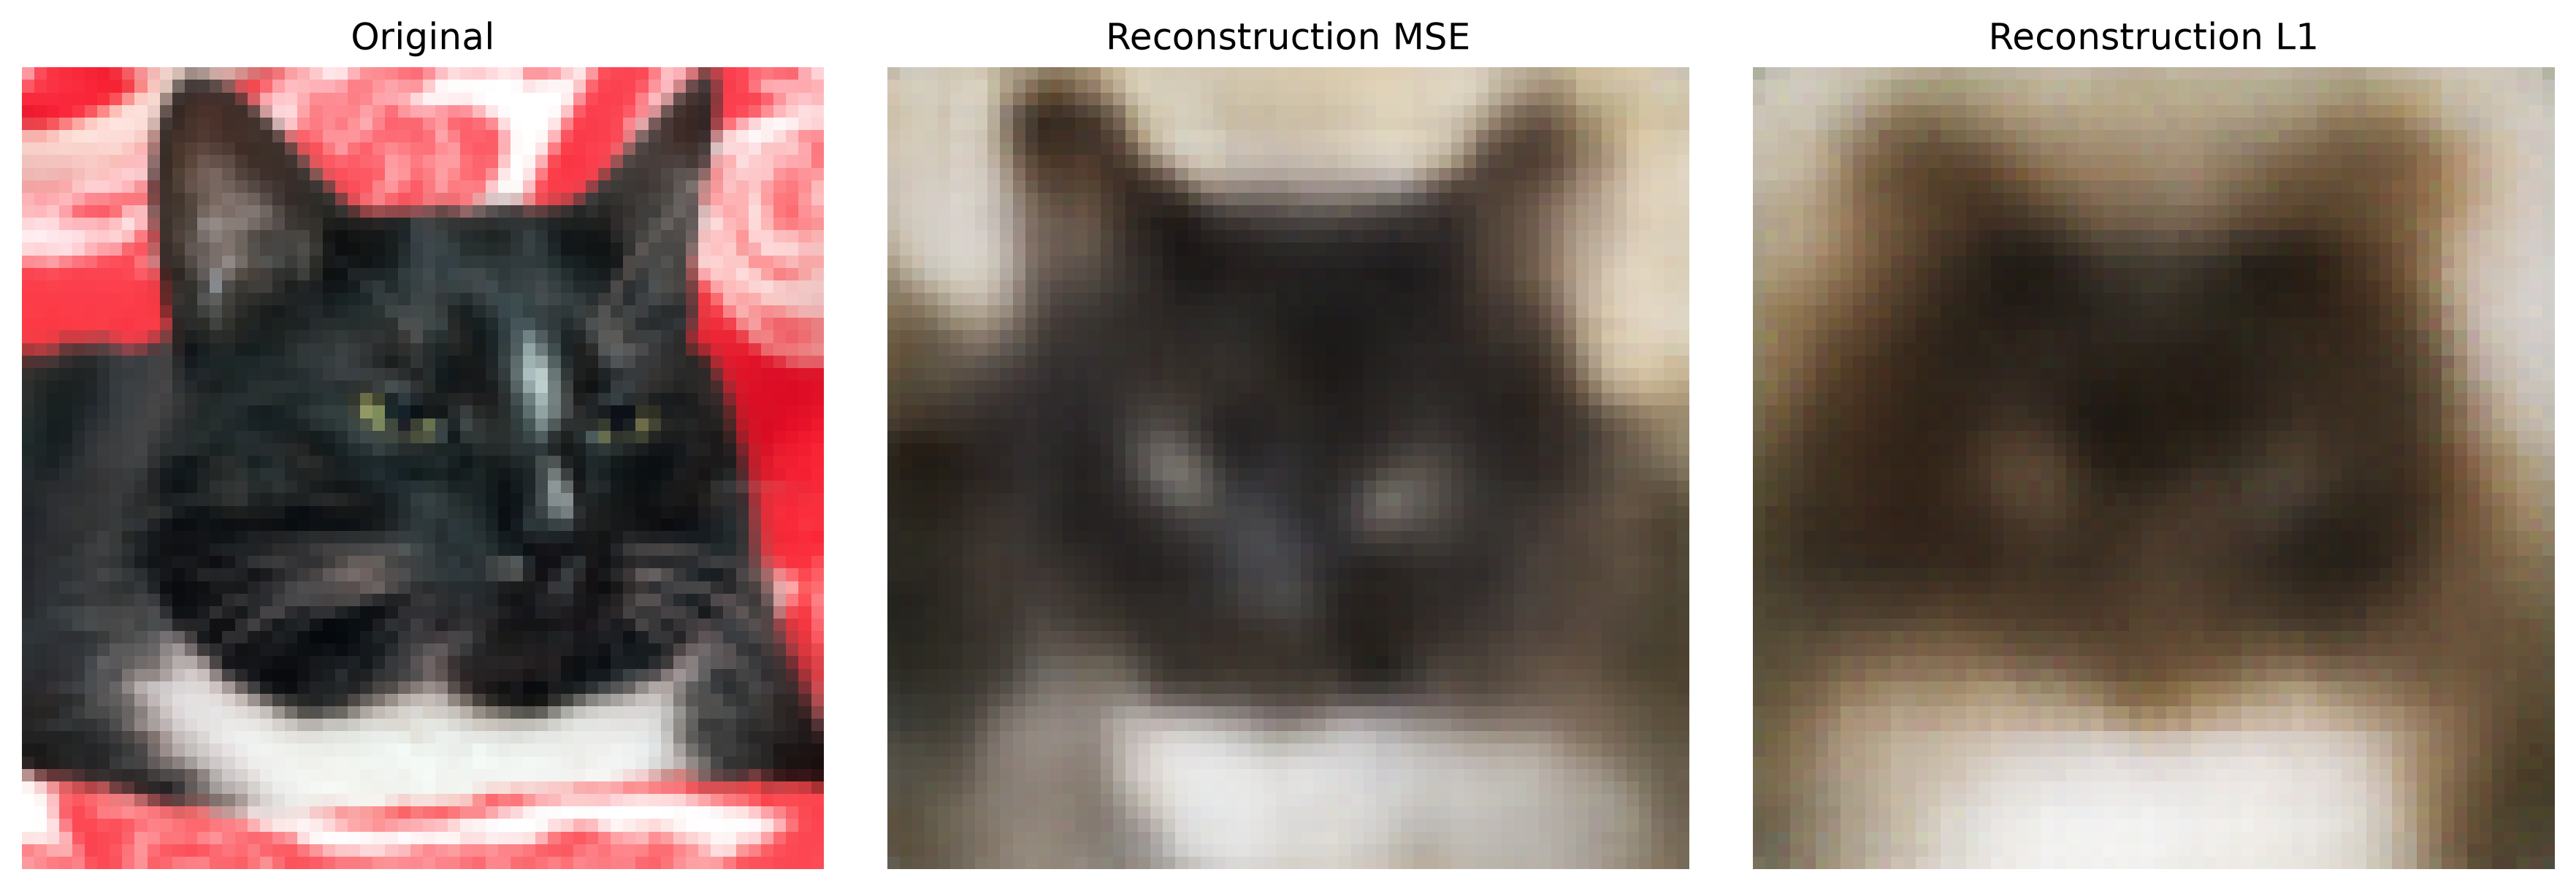
\includegraphics[width=\linewidth]{vector_latent/RQ2/L1/L1_b9/reconstruction_comparison_6.png}
        \caption*{}
    \end{subfigure}

    \caption{Examples of reconstruction quality for the spatial latent VAE stochastic.}
    \label{fig:spatial_latent_examples}
\end{figure}

\begin{figure}[H]
    \centering
    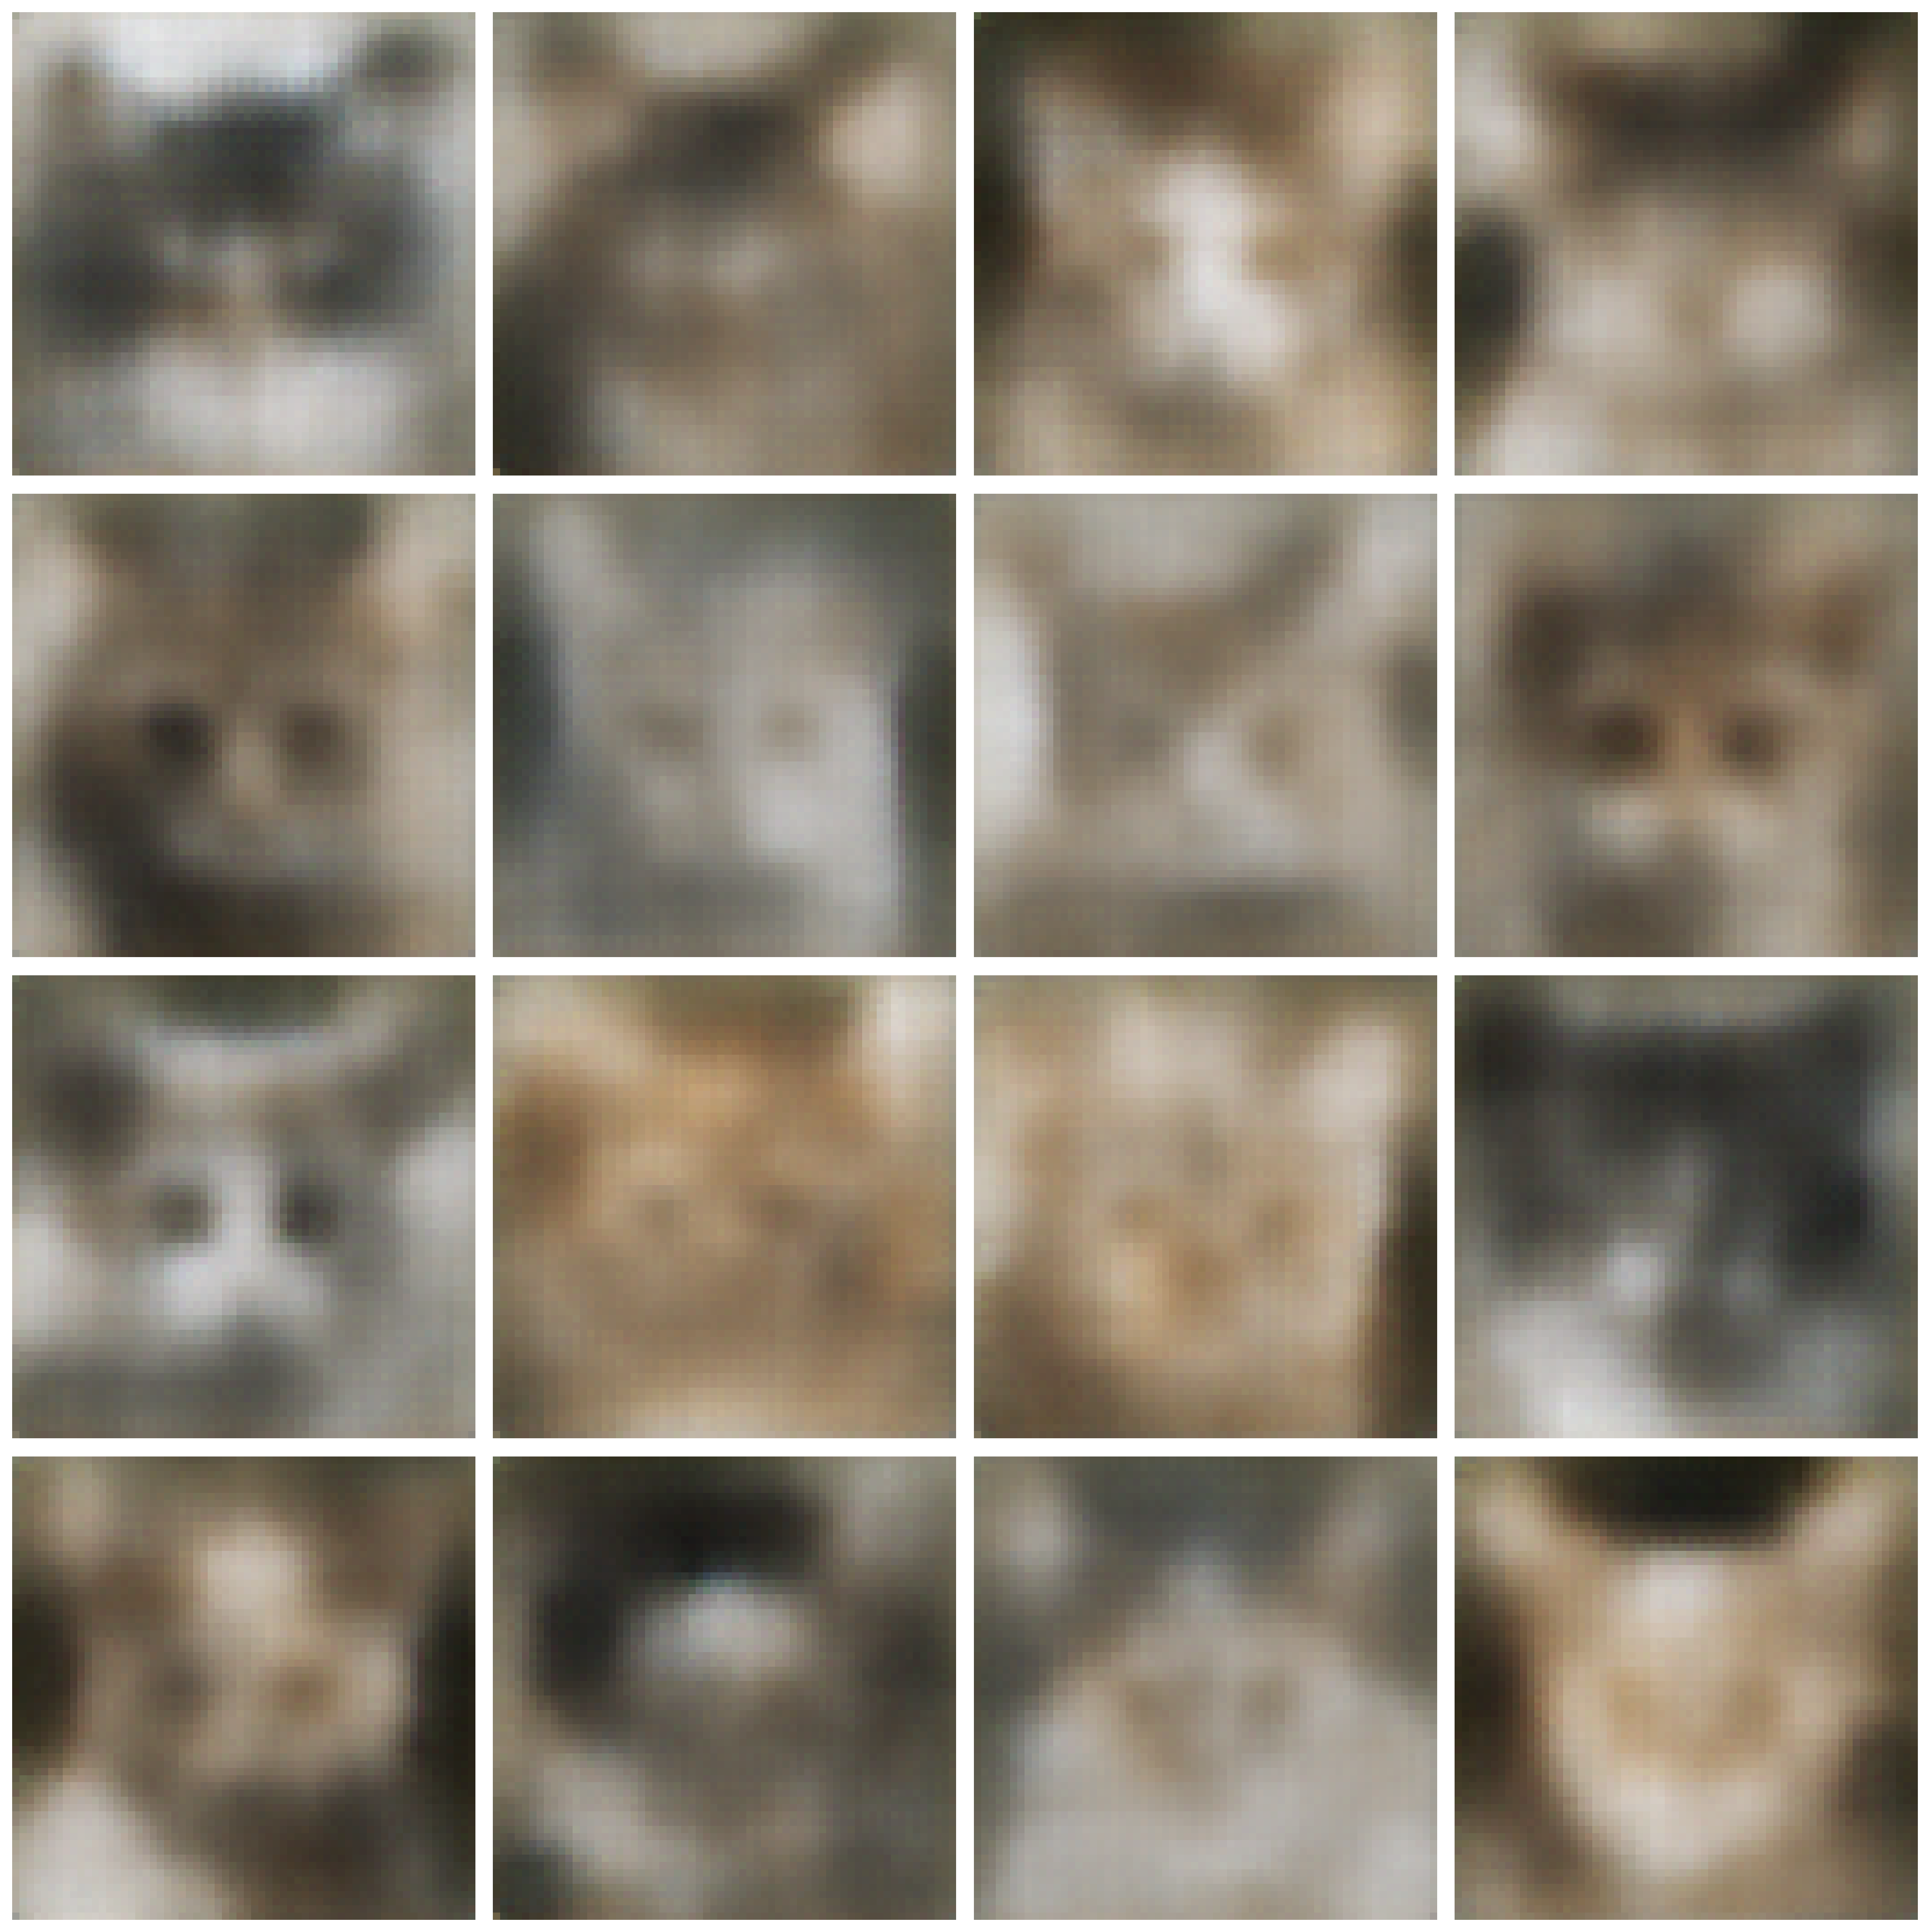
\includegraphics[width=0.4\linewidth]{vector_latent/RQ2/L1/L1_b9/generated_sample_x.png}
    \caption{Generated images.}
    \label{fig:placeholder}
\end{figure}

The resulting reconstructions were similar to, or slightly worse than, those obtained with the Gaussian reconstruction loss.

\textbf{Conclusion:} replacing the squared reconstruction error with L1 loss alone does not eliminate reconstruction blur. The initially sharper reconstruction obtained with $b=1$ was partly caused by the changed balance between the reconstruction and KL terms.


\subsection{Gaussian Reconstruction Loss with SSIM}

SSIM was tested as an additional structural reconstruction objective.

The combined reconstruction objective was

\[
L_{\mathrm{rec}}
=
L_{\mathrm{Gaussian}}
+
\lambda_{\mathrm{SSIM}}
(1-\mathrm{SSIM}).
\]

The scale of the Gaussian loss was much larger than the raw SSIM loss. Several weighting factors were therefore tested, including

\[
\lambda_{\mathrm{SSIM}} = 100
\qquad\text{and}\qquad
\lambda_{\mathrm{SSIM}} = 300.
\]

In some cases, SSIM slightly improved structural consistency or reduced blur. However, the improvement was not consistent across all images. In some cases no improvement was visible, while in others reconstruction accuracy became slightly worse.

\begin{figure}[H]
    \centering

    \begin{subfigure}{0.48\textwidth}
        \centering
        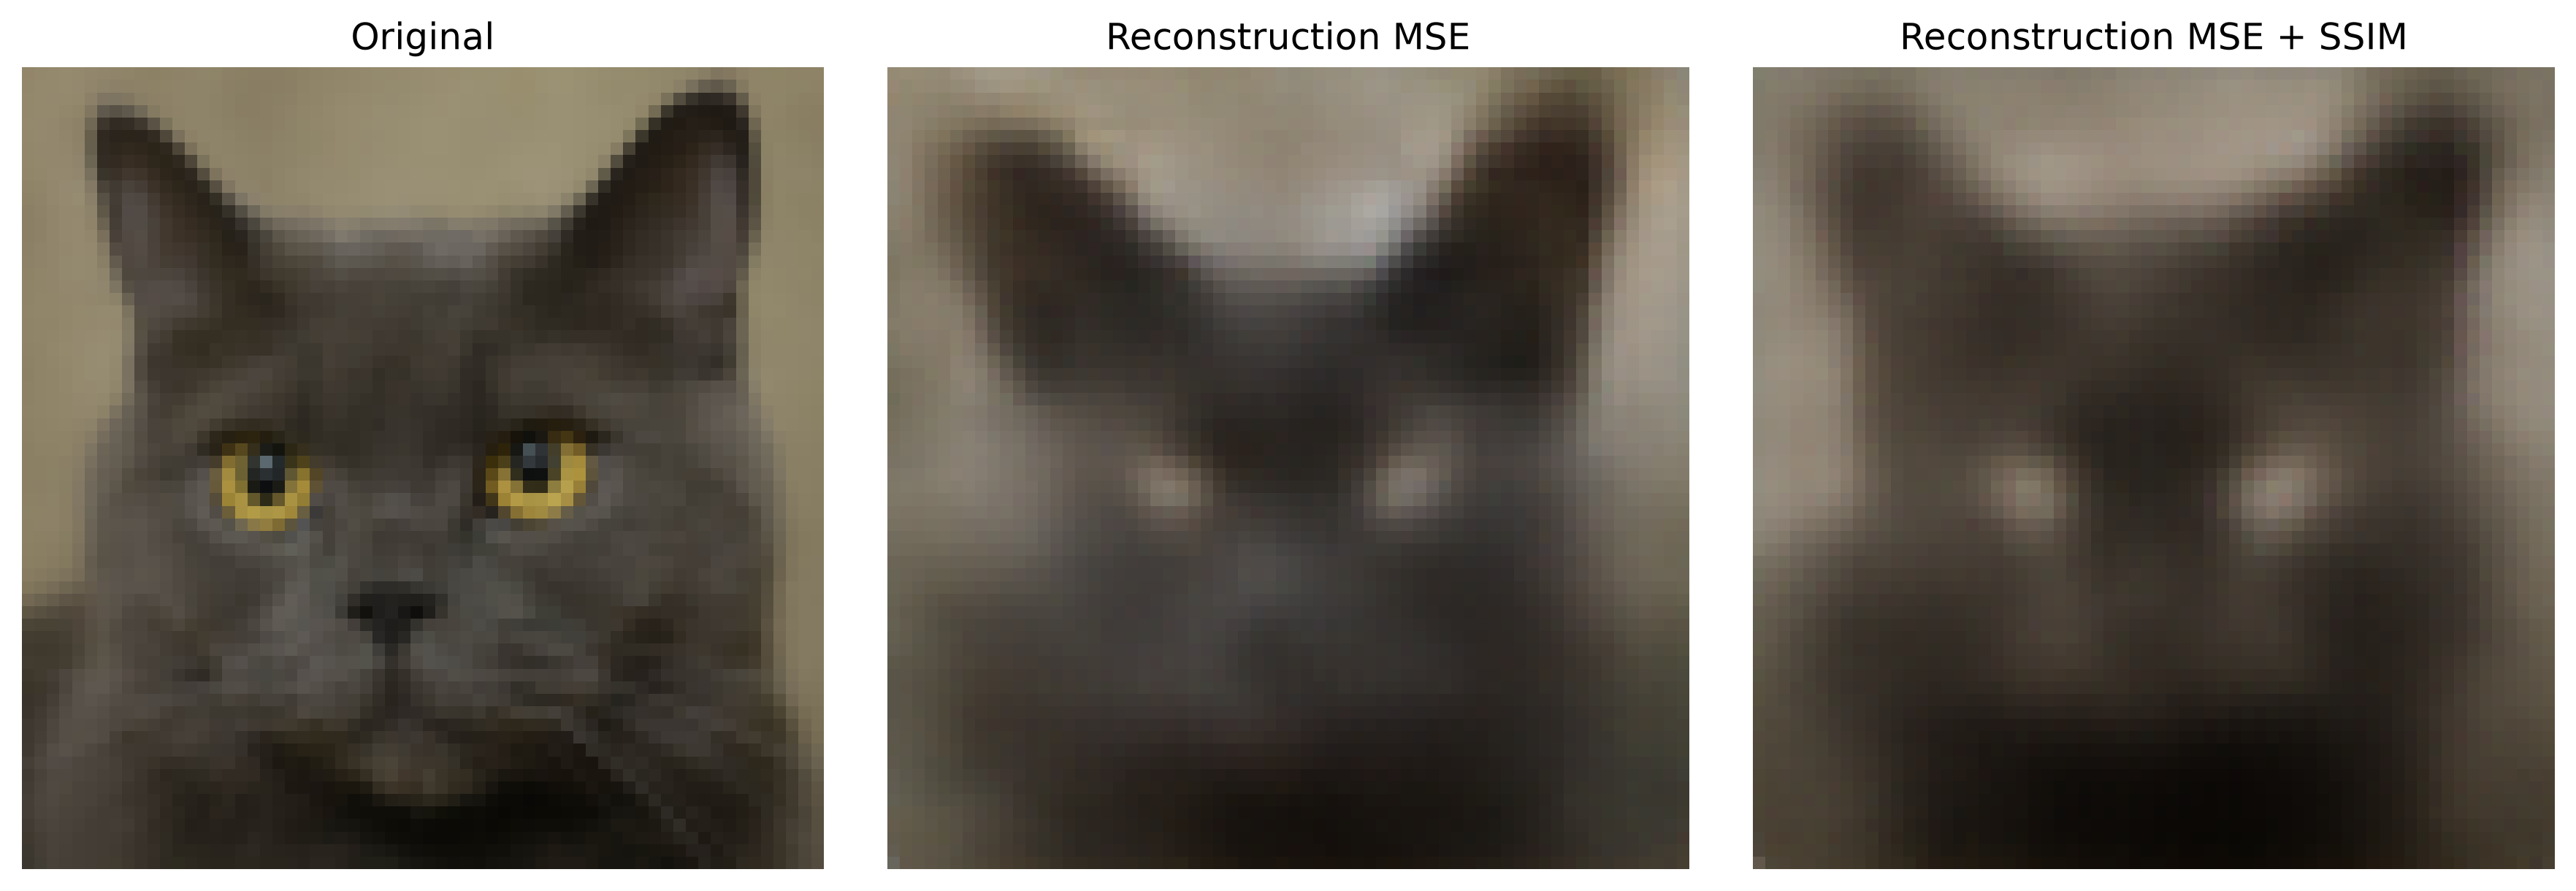
\includegraphics[width=\linewidth]{vector_latent/RQ2/SSIM/reconstruction_comparison_1.png}
        \caption*{}
    \end{subfigure}
    \hspace{0.02\textwidth}
    \begin{subfigure}{0.48\textwidth}
        \centering
        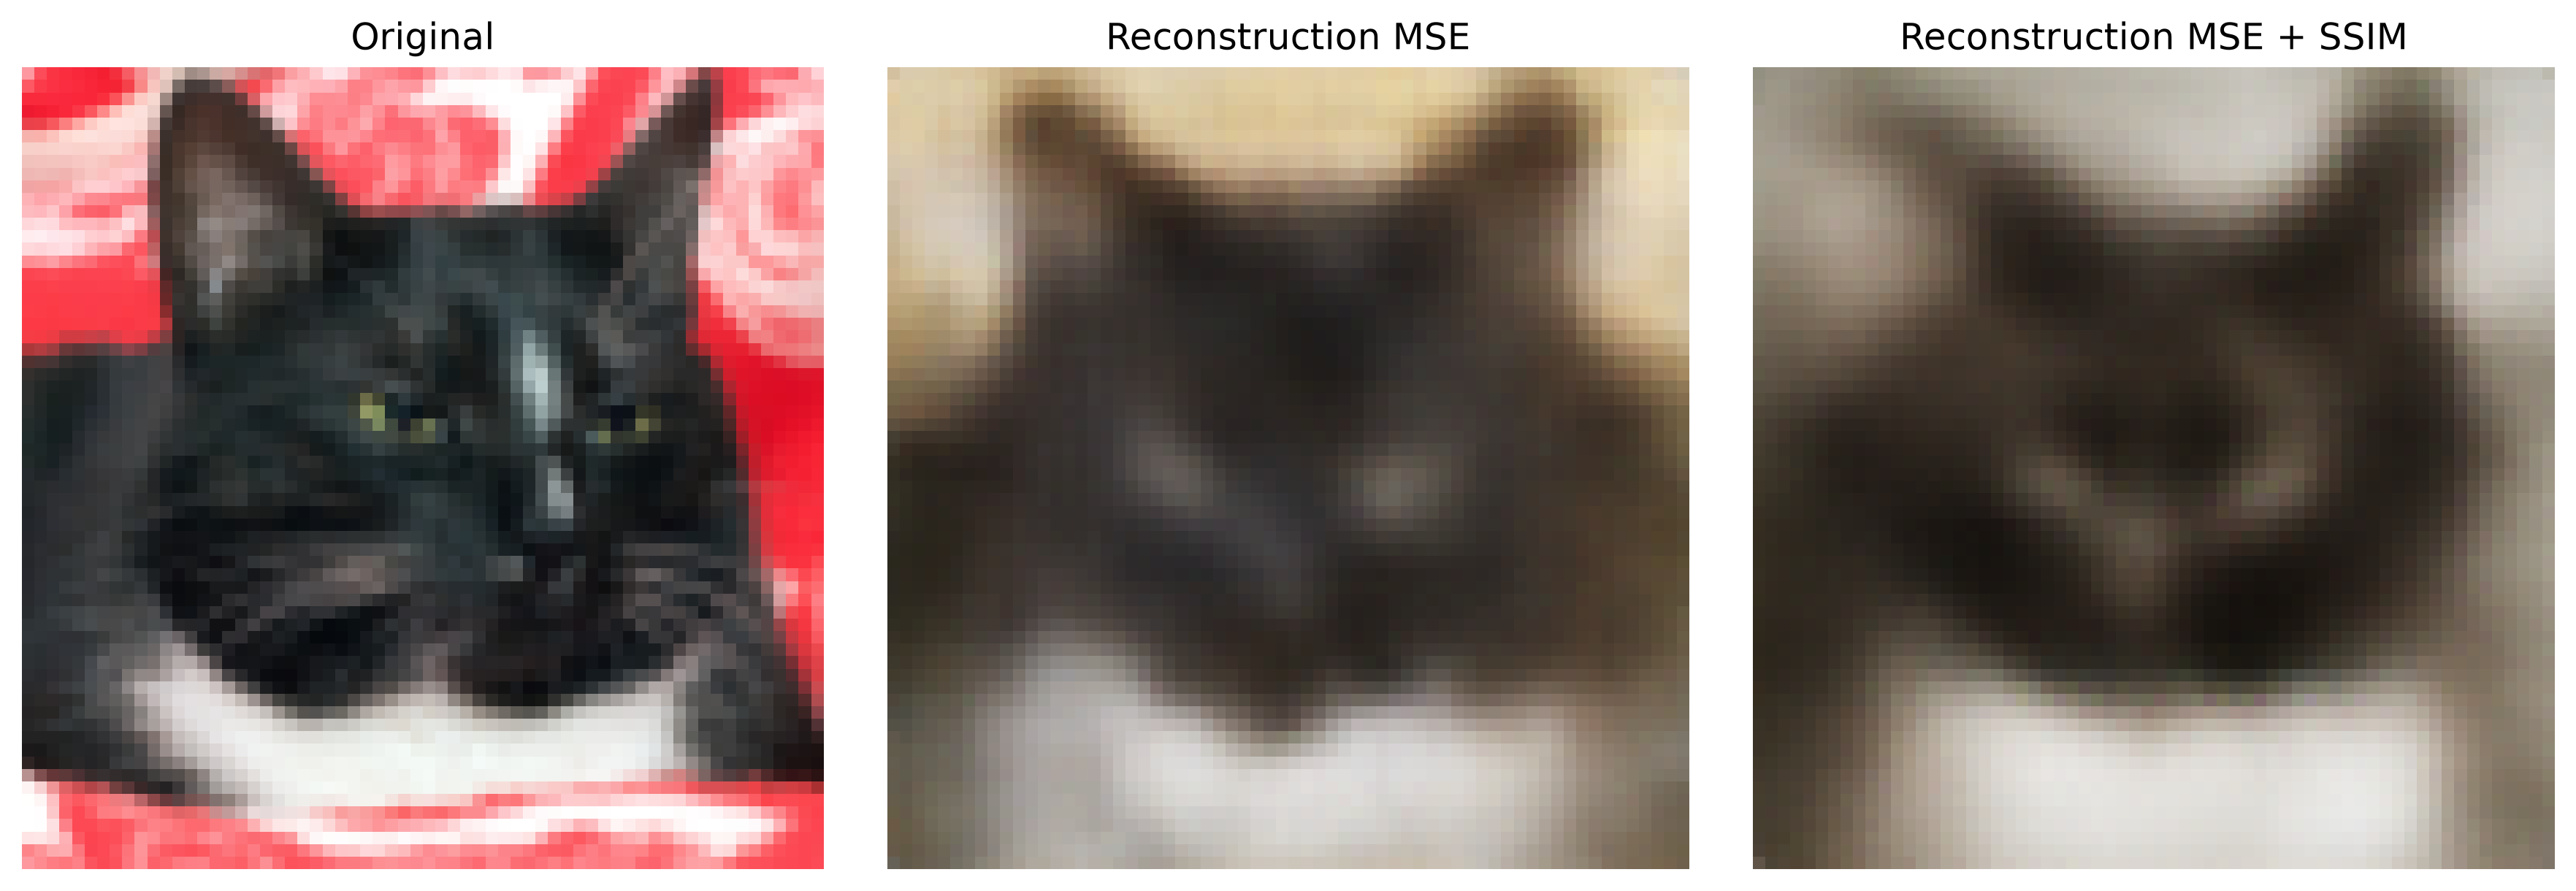
\includegraphics[width=\linewidth]{vector_latent/RQ2/SSIM/reconstruction_comparison_6.png}
        \caption*{}
    \end{subfigure}

    \caption{Examples of reconstruction quality for the spatial latent VAE stochastic.}
    \label{fig:generated l1}
\end{figure}

\textbf{Conclusion:} adding SSIM does not solve the main reconstruction blur problem and does not provide a consistent advantage over the Gaussian reconstruction objective.


\subsection{Overfitting Test on a Small Dataset}

An overfitting experiment was performed on a small subset of the dataset in order to determine whether the encoder--decoder architecture itself was capable of producing sharp reconstructions.

The experiment used the following configuration:

\[
\begin{aligned}
d_z &= 64, \\
\beta &= 0, \\
z &= \mu, \\
L_{\mathrm{rec}} &= L_{\mathrm{Gaussian}}.
\end{aligned}
\]

Stochastic latent sampling was disabled and the model was trained for a large number of epochs in order to intentionally overfit the small dataset.

The resulting reconstructions contained substantially more detail and showed only minimal blur.

\begin{figure}[H]
    \centering

    \begin{subfigure}{0.48\textwidth}
        \centering
        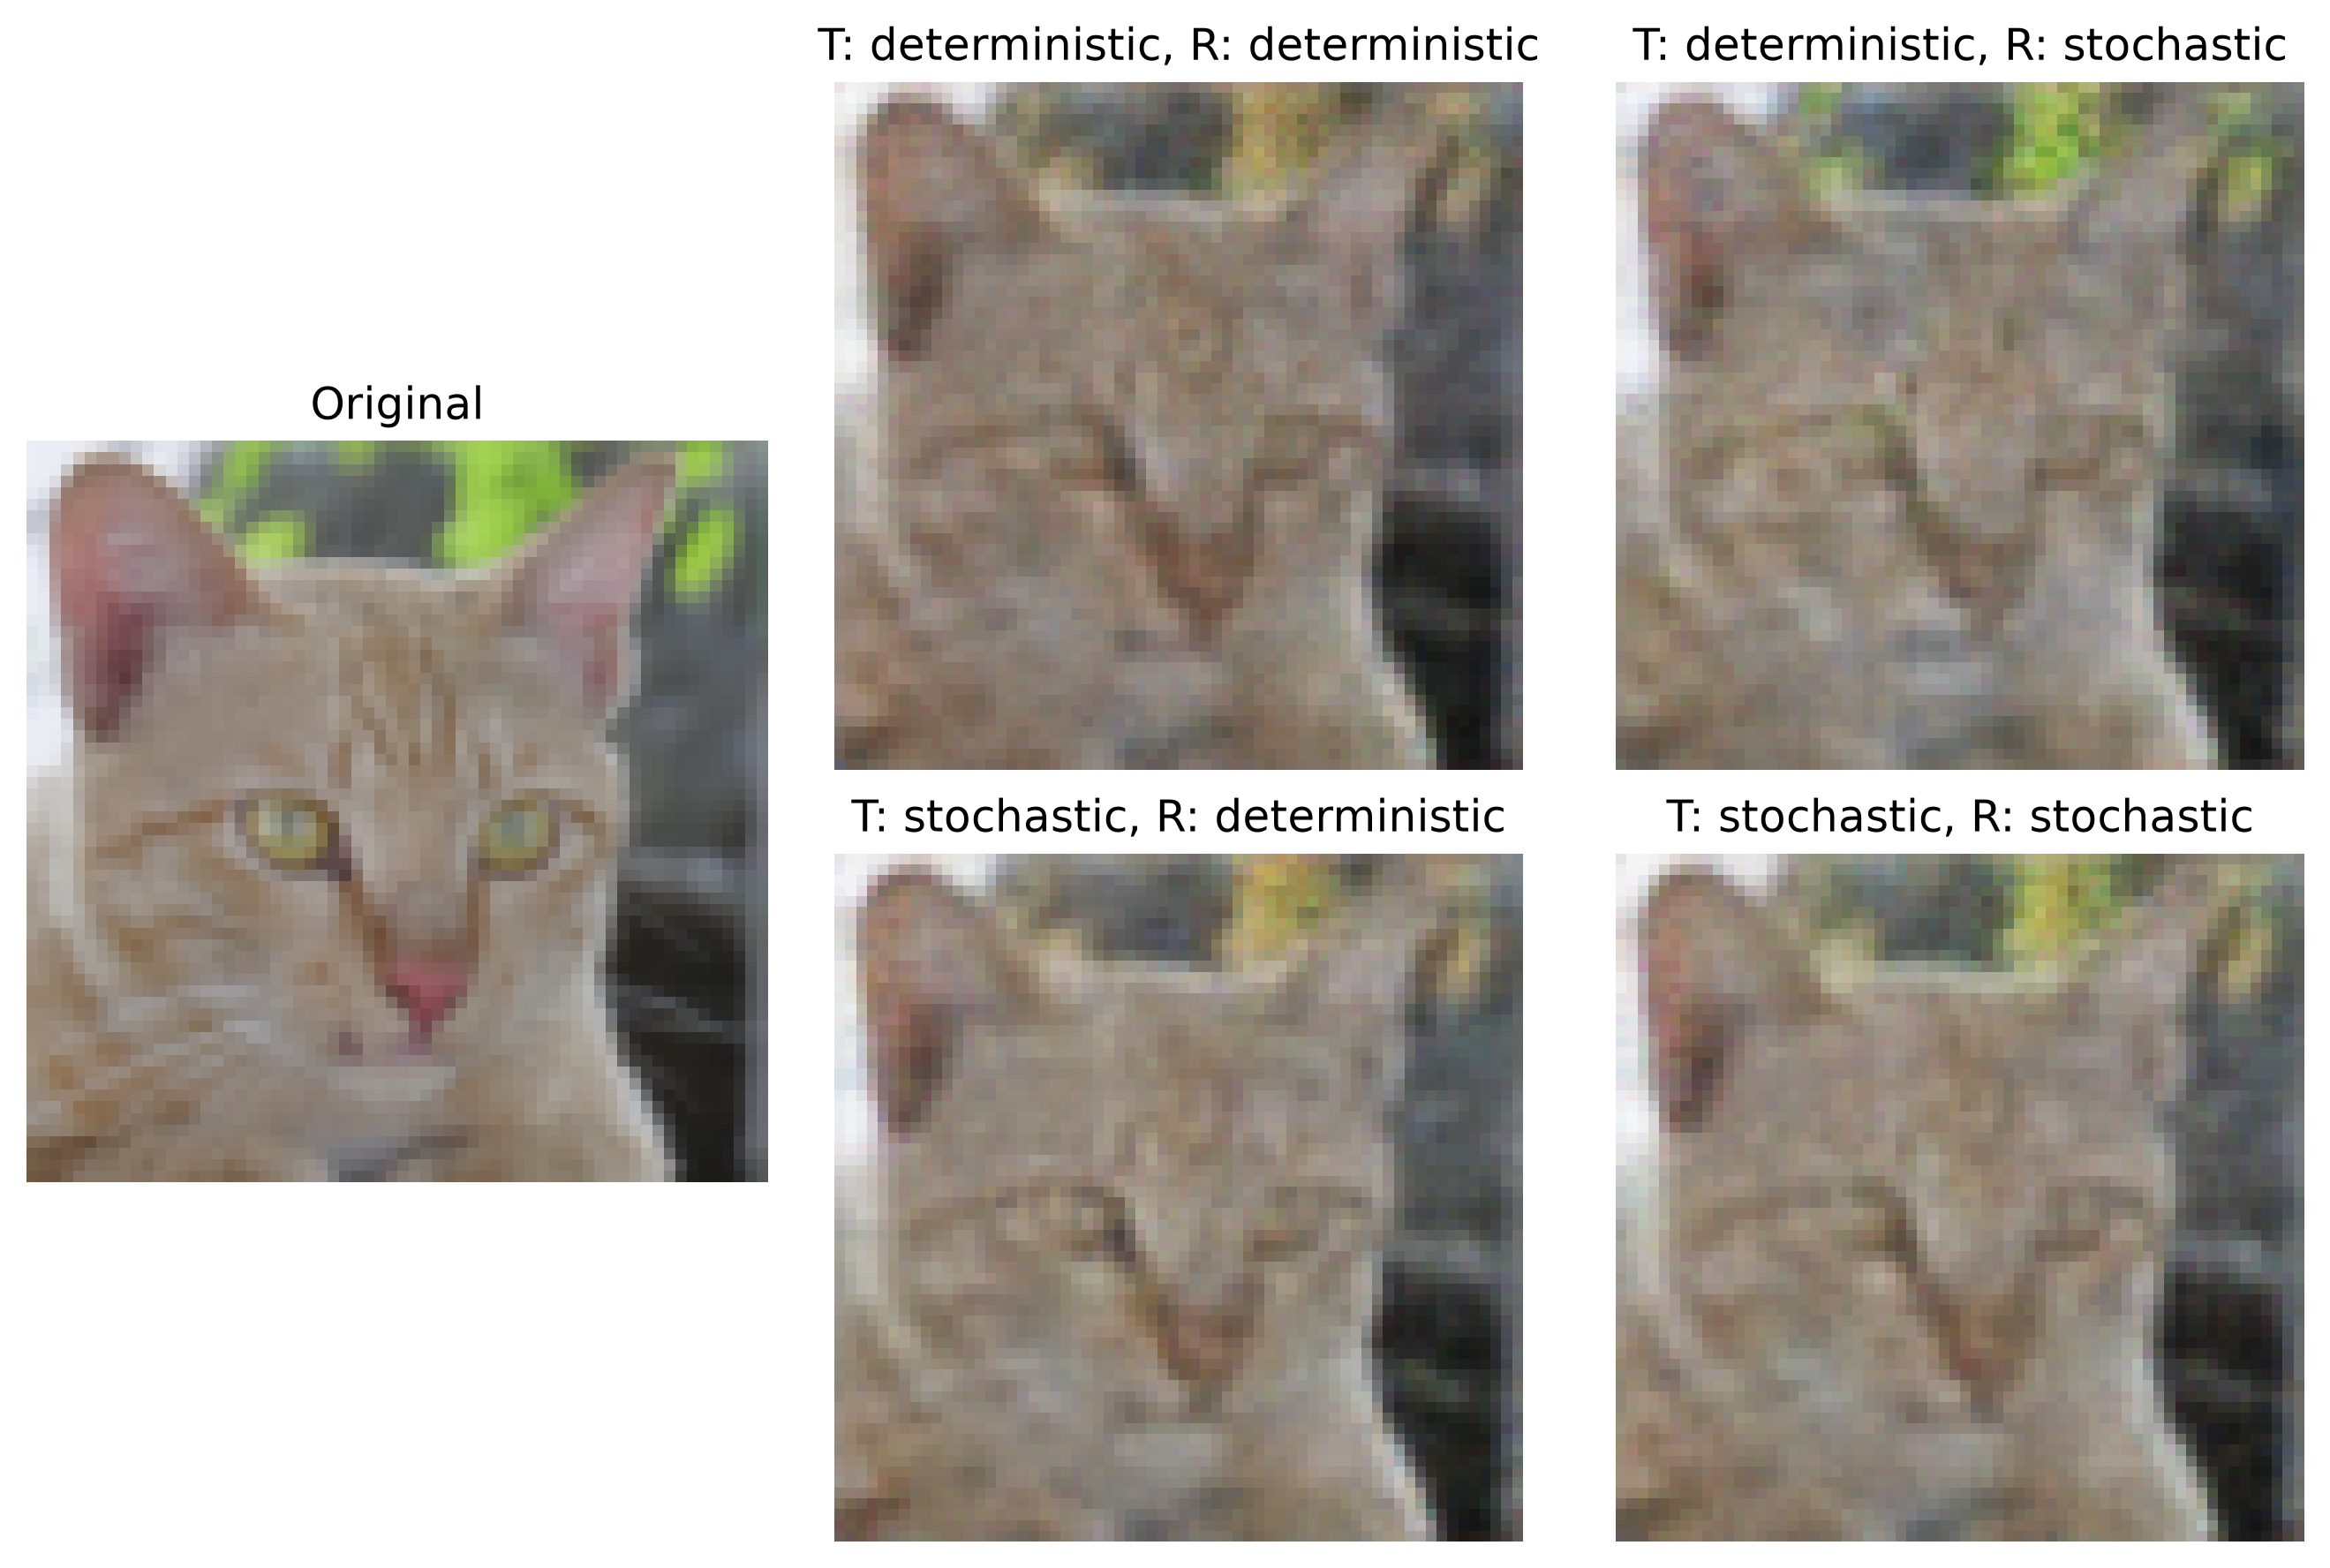
\includegraphics[width=\linewidth]{vector_latent/RQ2/overfitting_beta0_500epok/reconstruction_grid_9.png}
        \caption*{}
    \end{subfigure}
    \hspace{0.02\textwidth}
    \begin{subfigure}{0.48\textwidth}
        \centering
        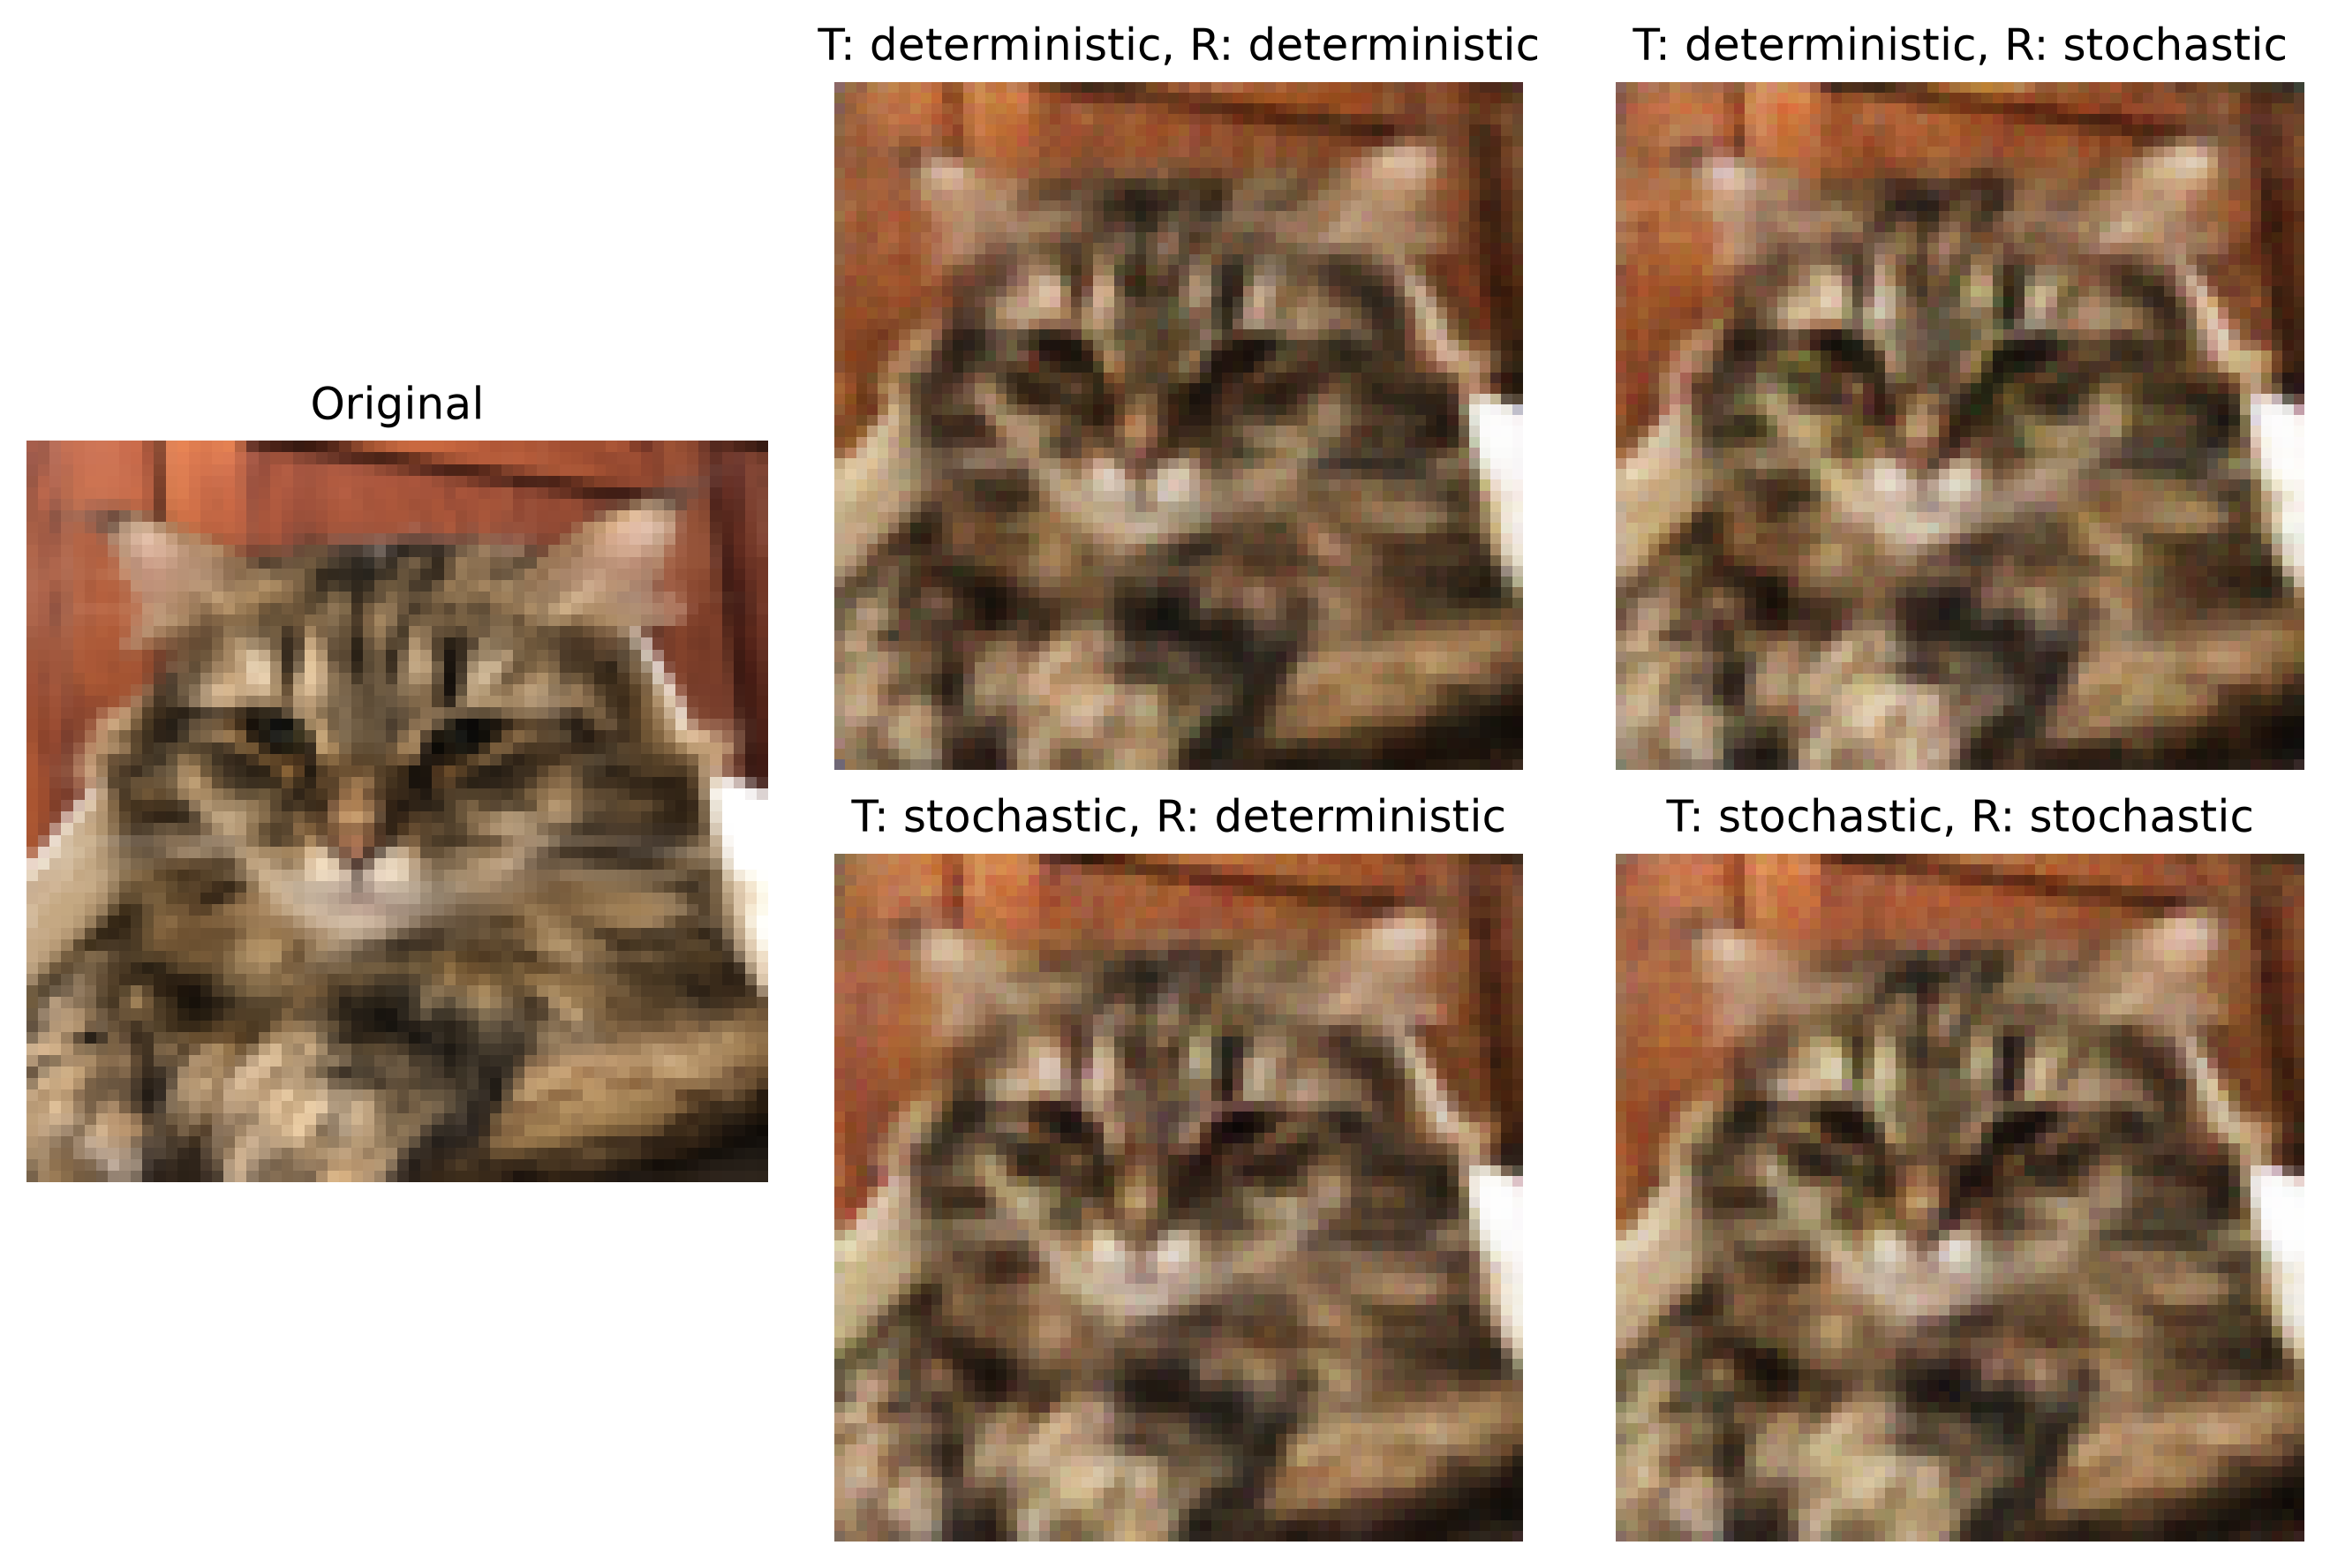
\includegraphics[width=\linewidth]{vector_latent/RQ2/overfitting_beta0_500epok/reconstruction_grid_13.png}
        \caption*{}
    \end{subfigure}

    \caption{Examples of reconstruction quality for the spatial latent VAE stochastic.}
    \label{fig:spatial_latent_examples}
\end{figure}

\textbf{Conclusion:} the current encoder--decoder architecture is capable of producing relatively sharp reconstructions. Therefore, the reconstruction blur observed in normal training cannot be explained simply by an inability of the architecture to reconstruct detailed images.

\subsection{Small Dataset with KL Regularization}

The small-dataset overfitting experiment was repeated with $\beta=1$, while the latent representation remained deterministic:

\[
z = \mu.
\]

The reconstructions became slightly more blurred than in the $\beta=0$ experiment, but the degradation was relatively small.

\begin{figure}[H]
    \centering

    \begin{subfigure}{0.48\textwidth}
        \centering
        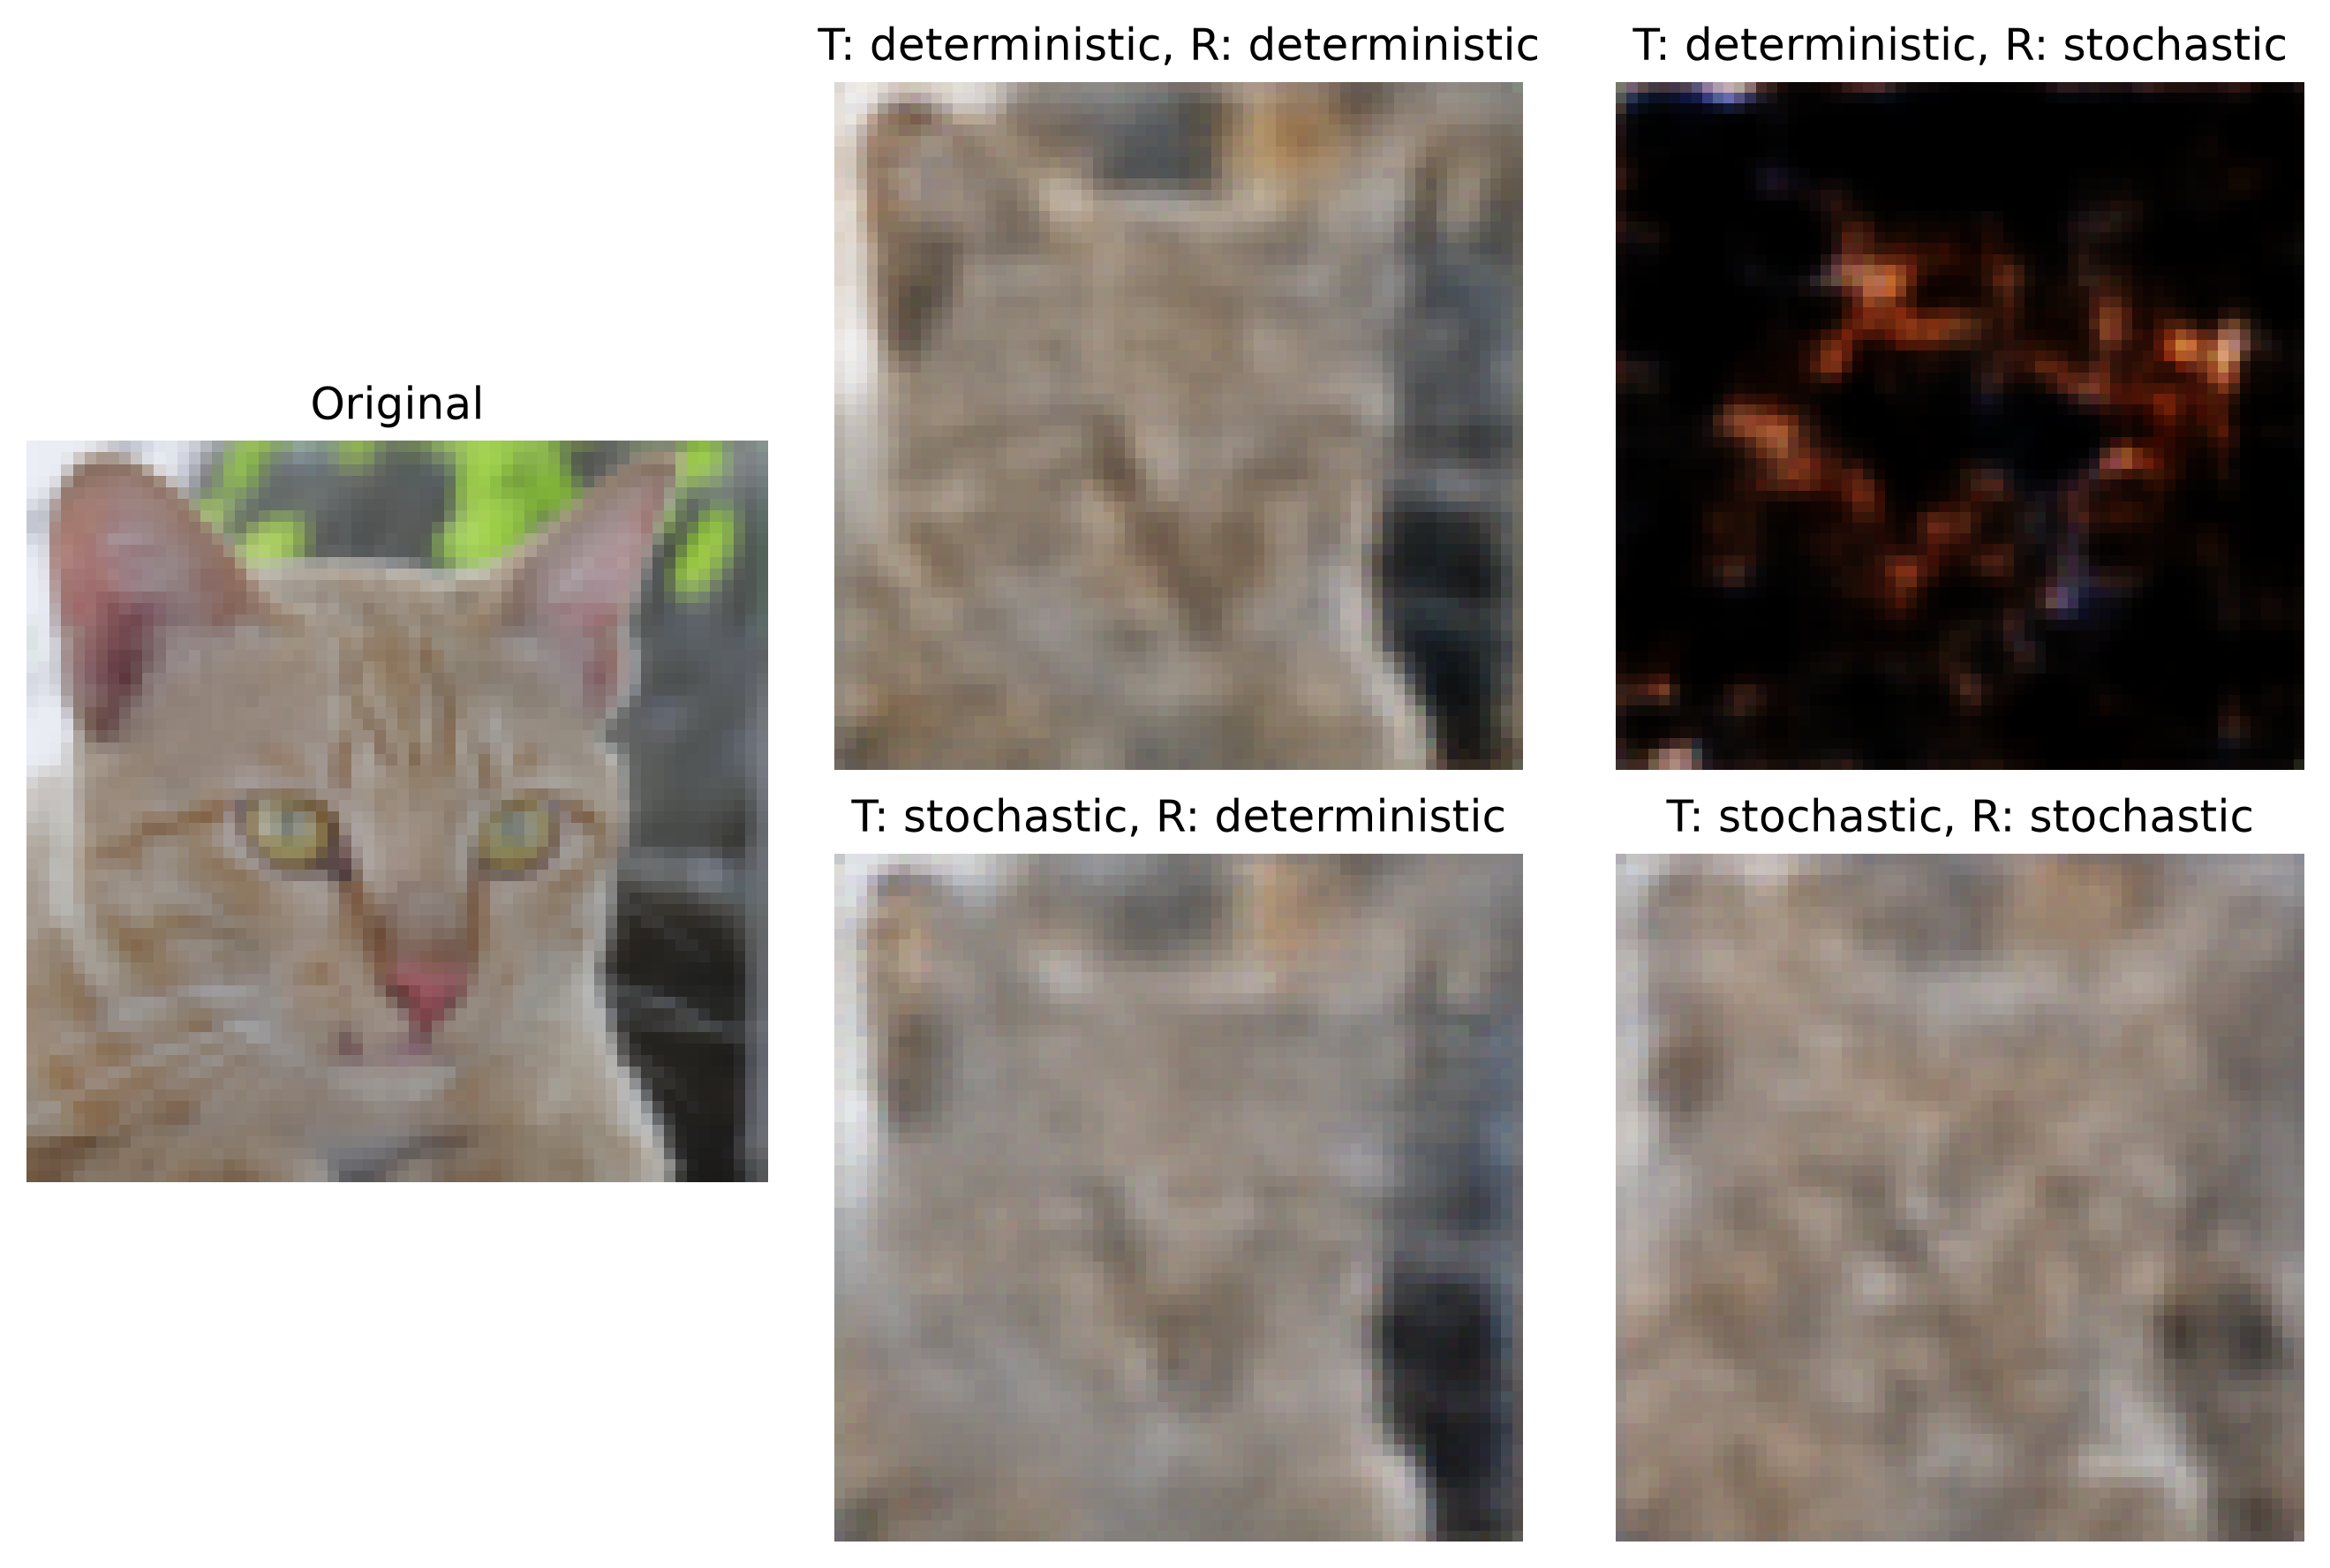
\includegraphics[width=\linewidth]{vector_latent/RQ2/overfitting_beta1_500epok/reconstruction_grid_9.png}
        \caption*{}
    \end{subfigure}
    \hspace{0.02\textwidth}
    \begin{subfigure}{0.48\textwidth}
        \centering
        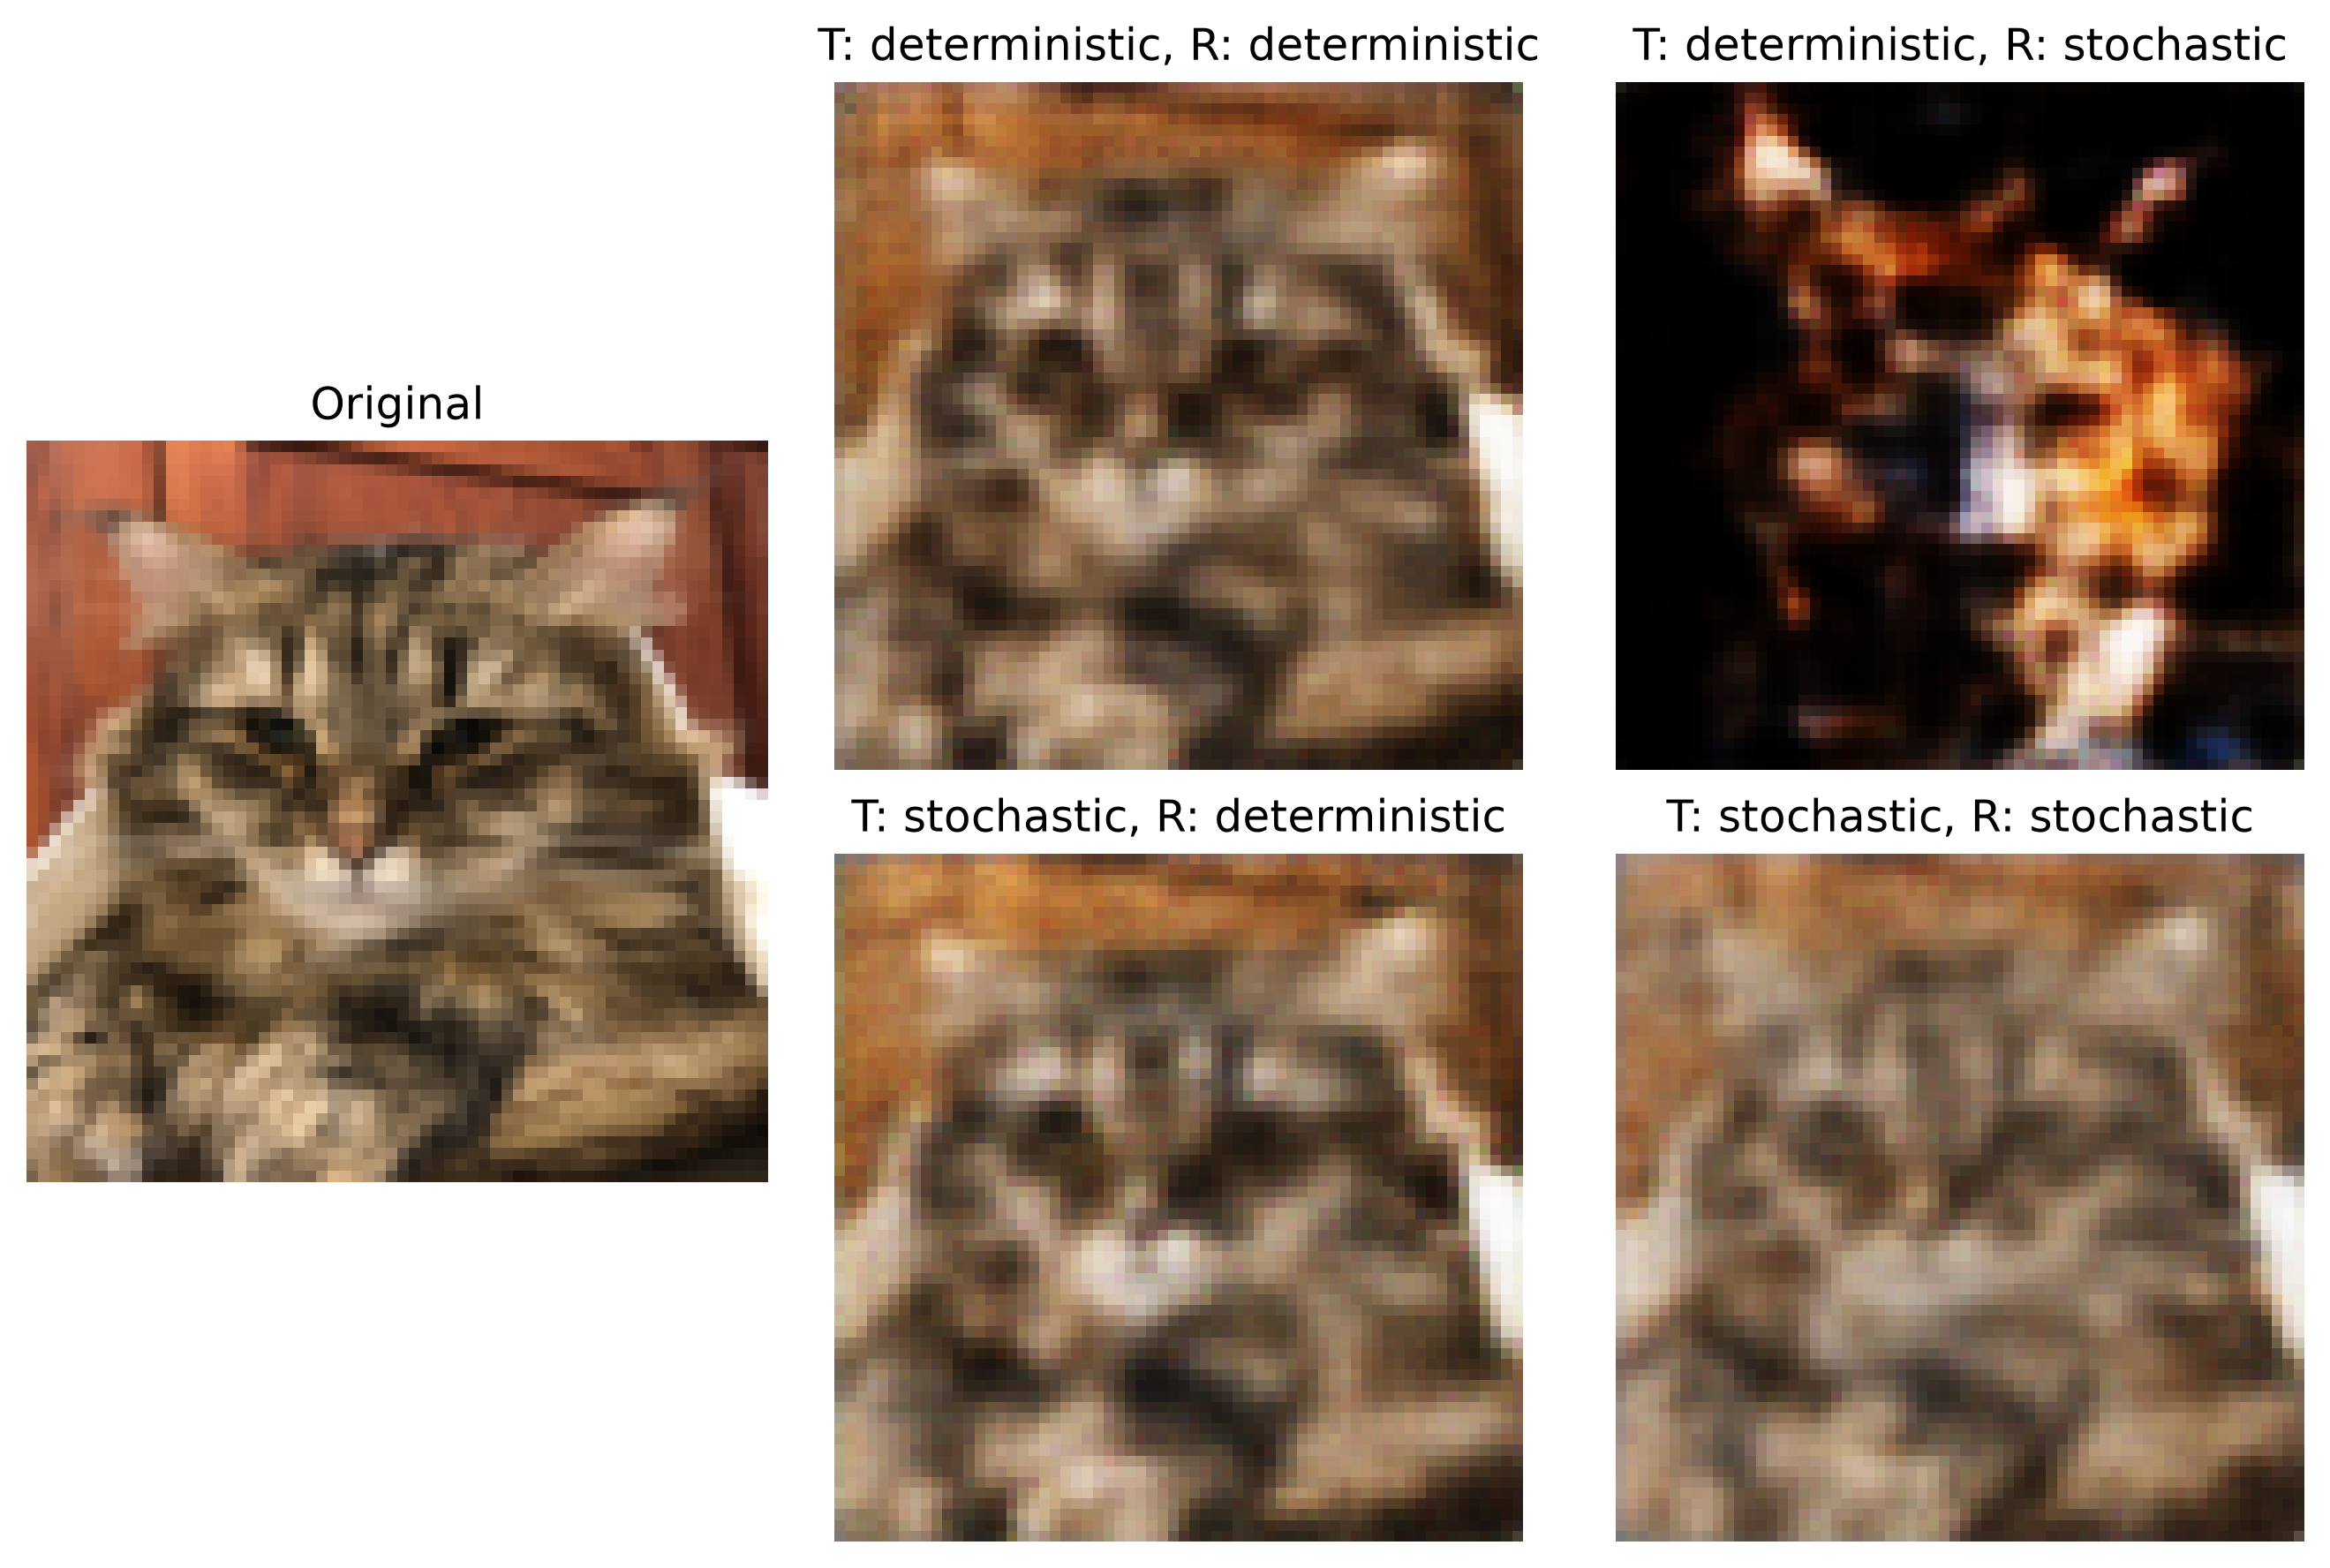
\includegraphics[width=\linewidth]{vector_latent/RQ2/overfitting_beta1_500epok/reconstruction_grid_13.png}
        \caption*{}
    \end{subfigure}
\end{figure}

\textbf{Conclusion:} KL regularization contributes to reconstruction degradation, but KL alone does not fully explain the strong blur observed when training on the full dataset.


\subsection{Full Dataset without KL Regularization}

The deterministic reconstruction experiment was then repeated on the full dataset using the same basic setup:

\[
\begin{aligned}
d_z &= 64, \\
\beta &= 0, \\
z &= \mu, \\
L_{\mathrm{rec}} &= L_{\mathrm{Gaussian}}.
\end{aligned}
\]

Thus, both KL regularization and stochastic latent sampling were removed from the training objective.

Despite this, reconstruction blur increased substantially for some images compared with the small-dataset overfitting experiment.

This indicates that the model can accurately reconstruct a small number of images, but representing the full variability of the dataset through the same latent representation is considerably more difficult.


\begin{figure}[H]
    \centering

    \begin{subfigure}{0.48\textwidth}
        \centering
        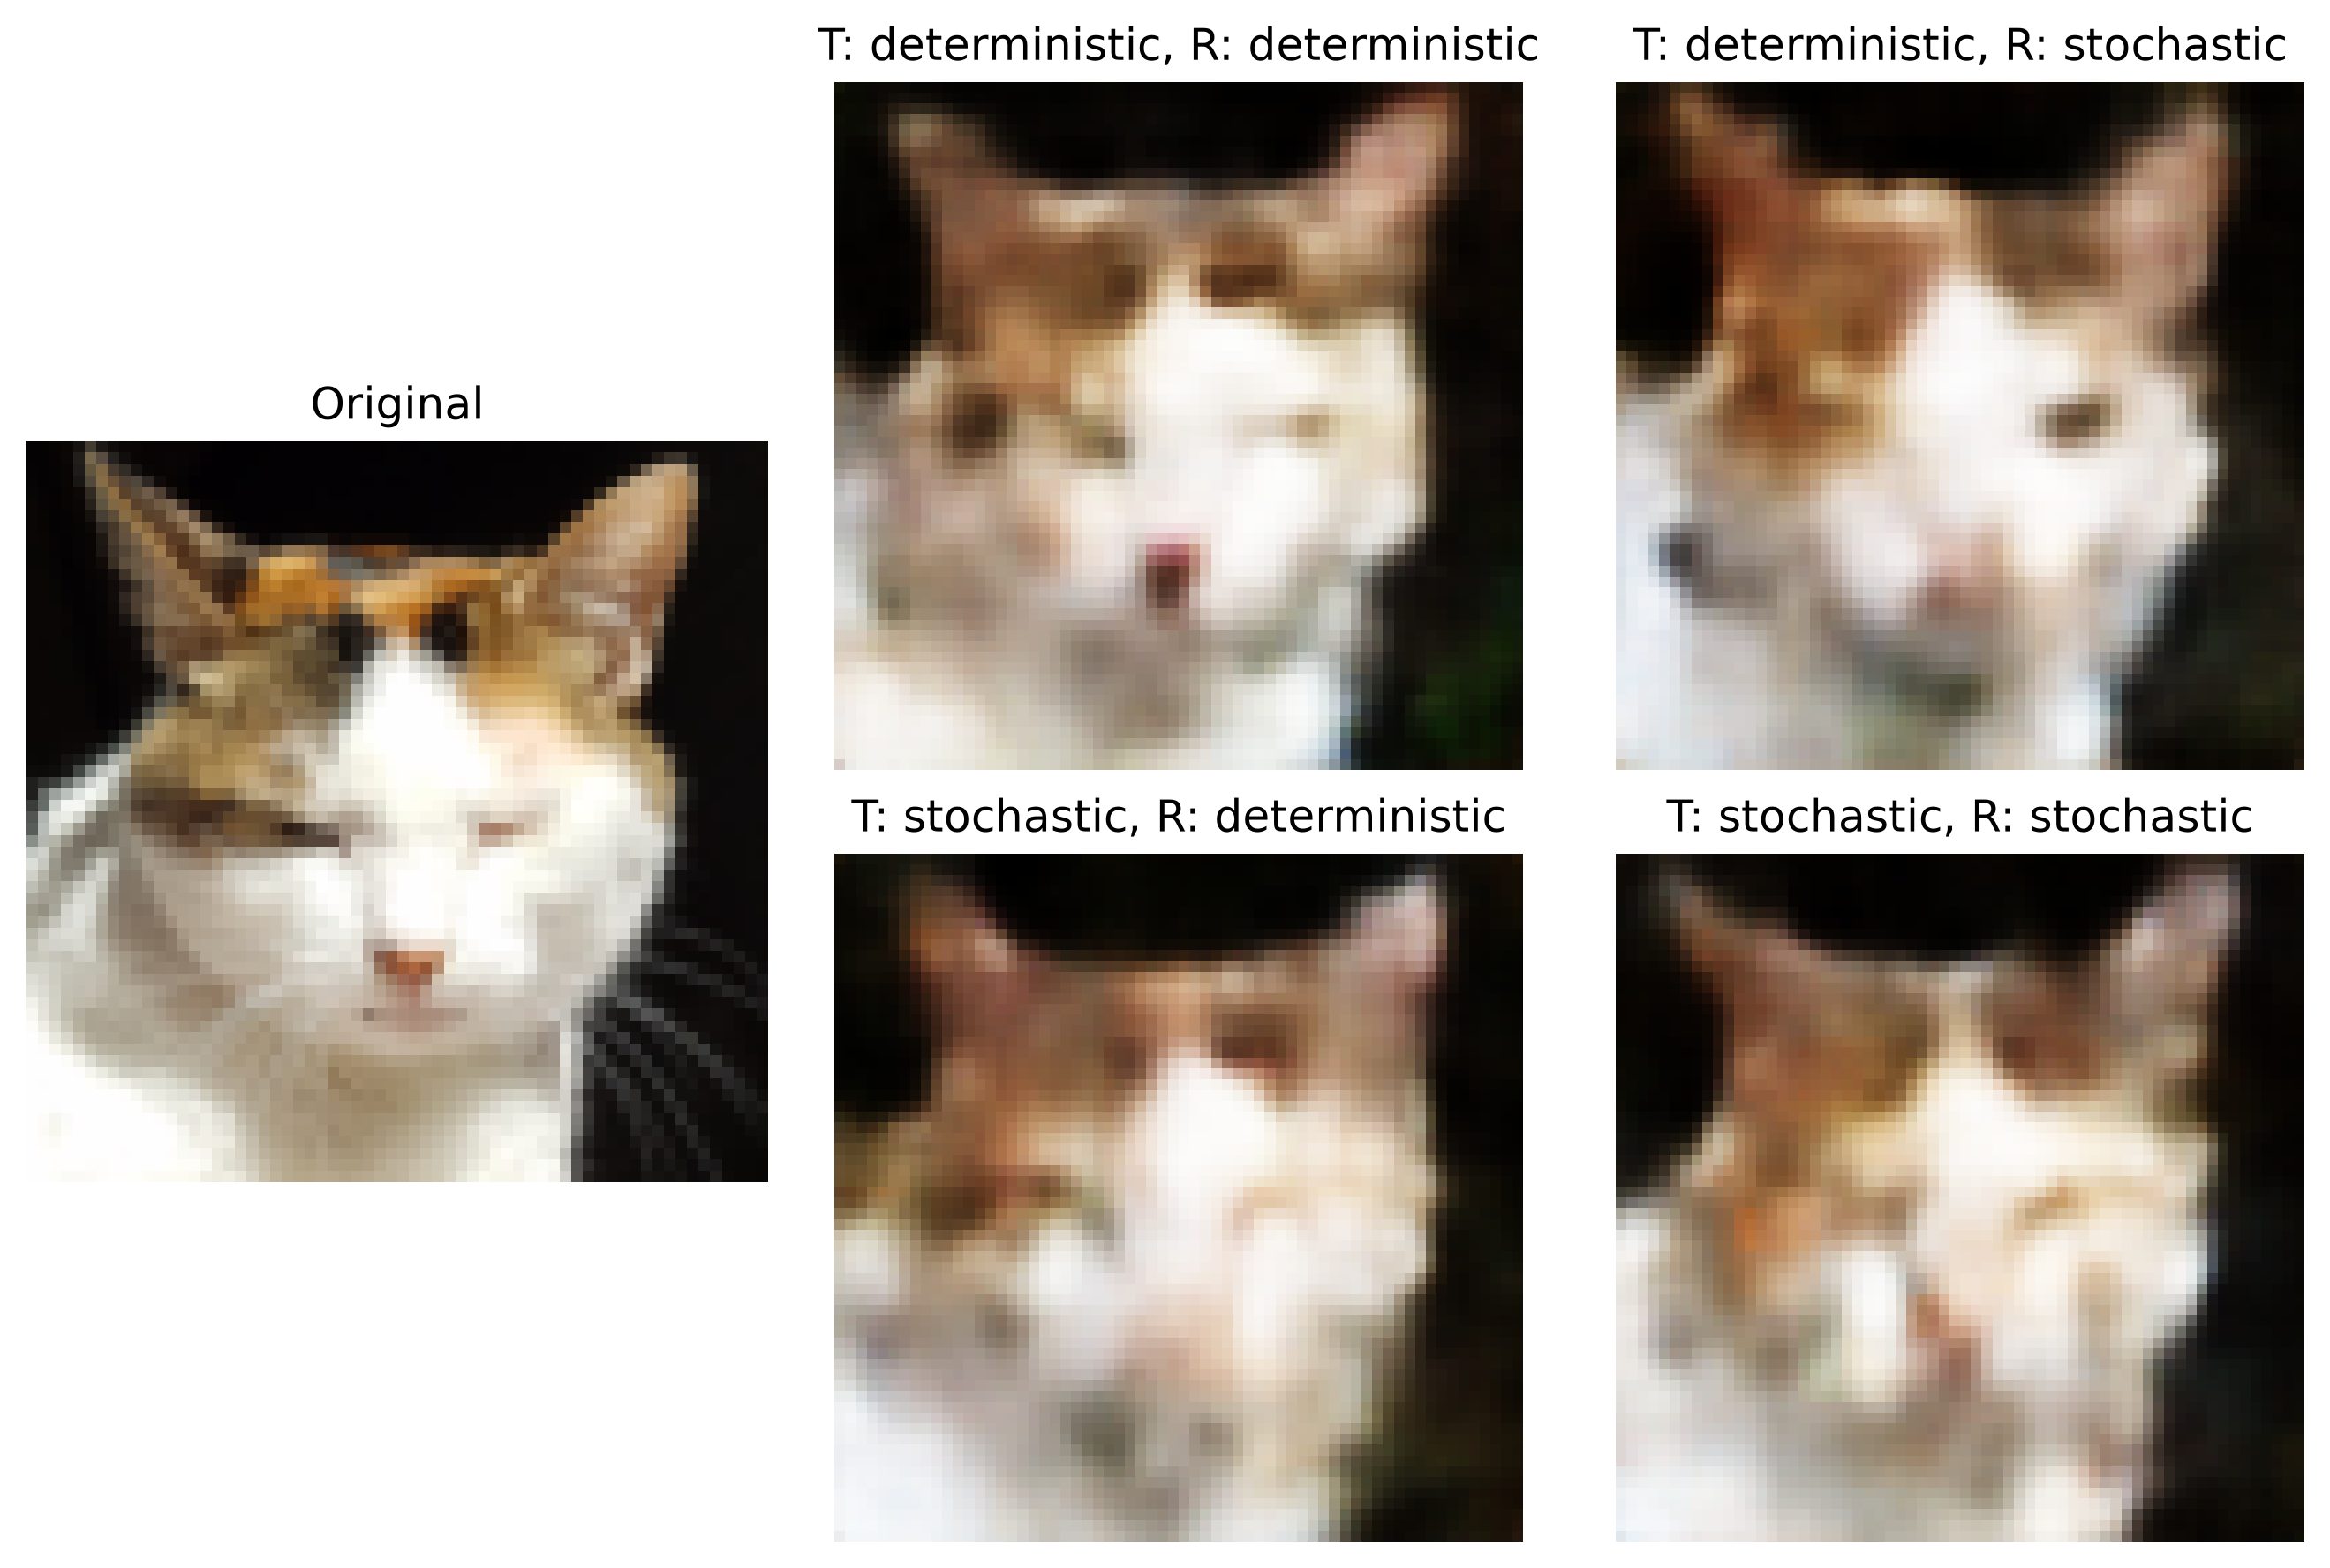
\includegraphics[width=\linewidth]{vector_latent/RQ2/full_dataset_100epok_beta0/reconstruction_grid_0.png}
        \caption*{}
    \end{subfigure}
    \hspace{0.02\textwidth}
    \begin{subfigure}{0.48\textwidth}
        \centering
        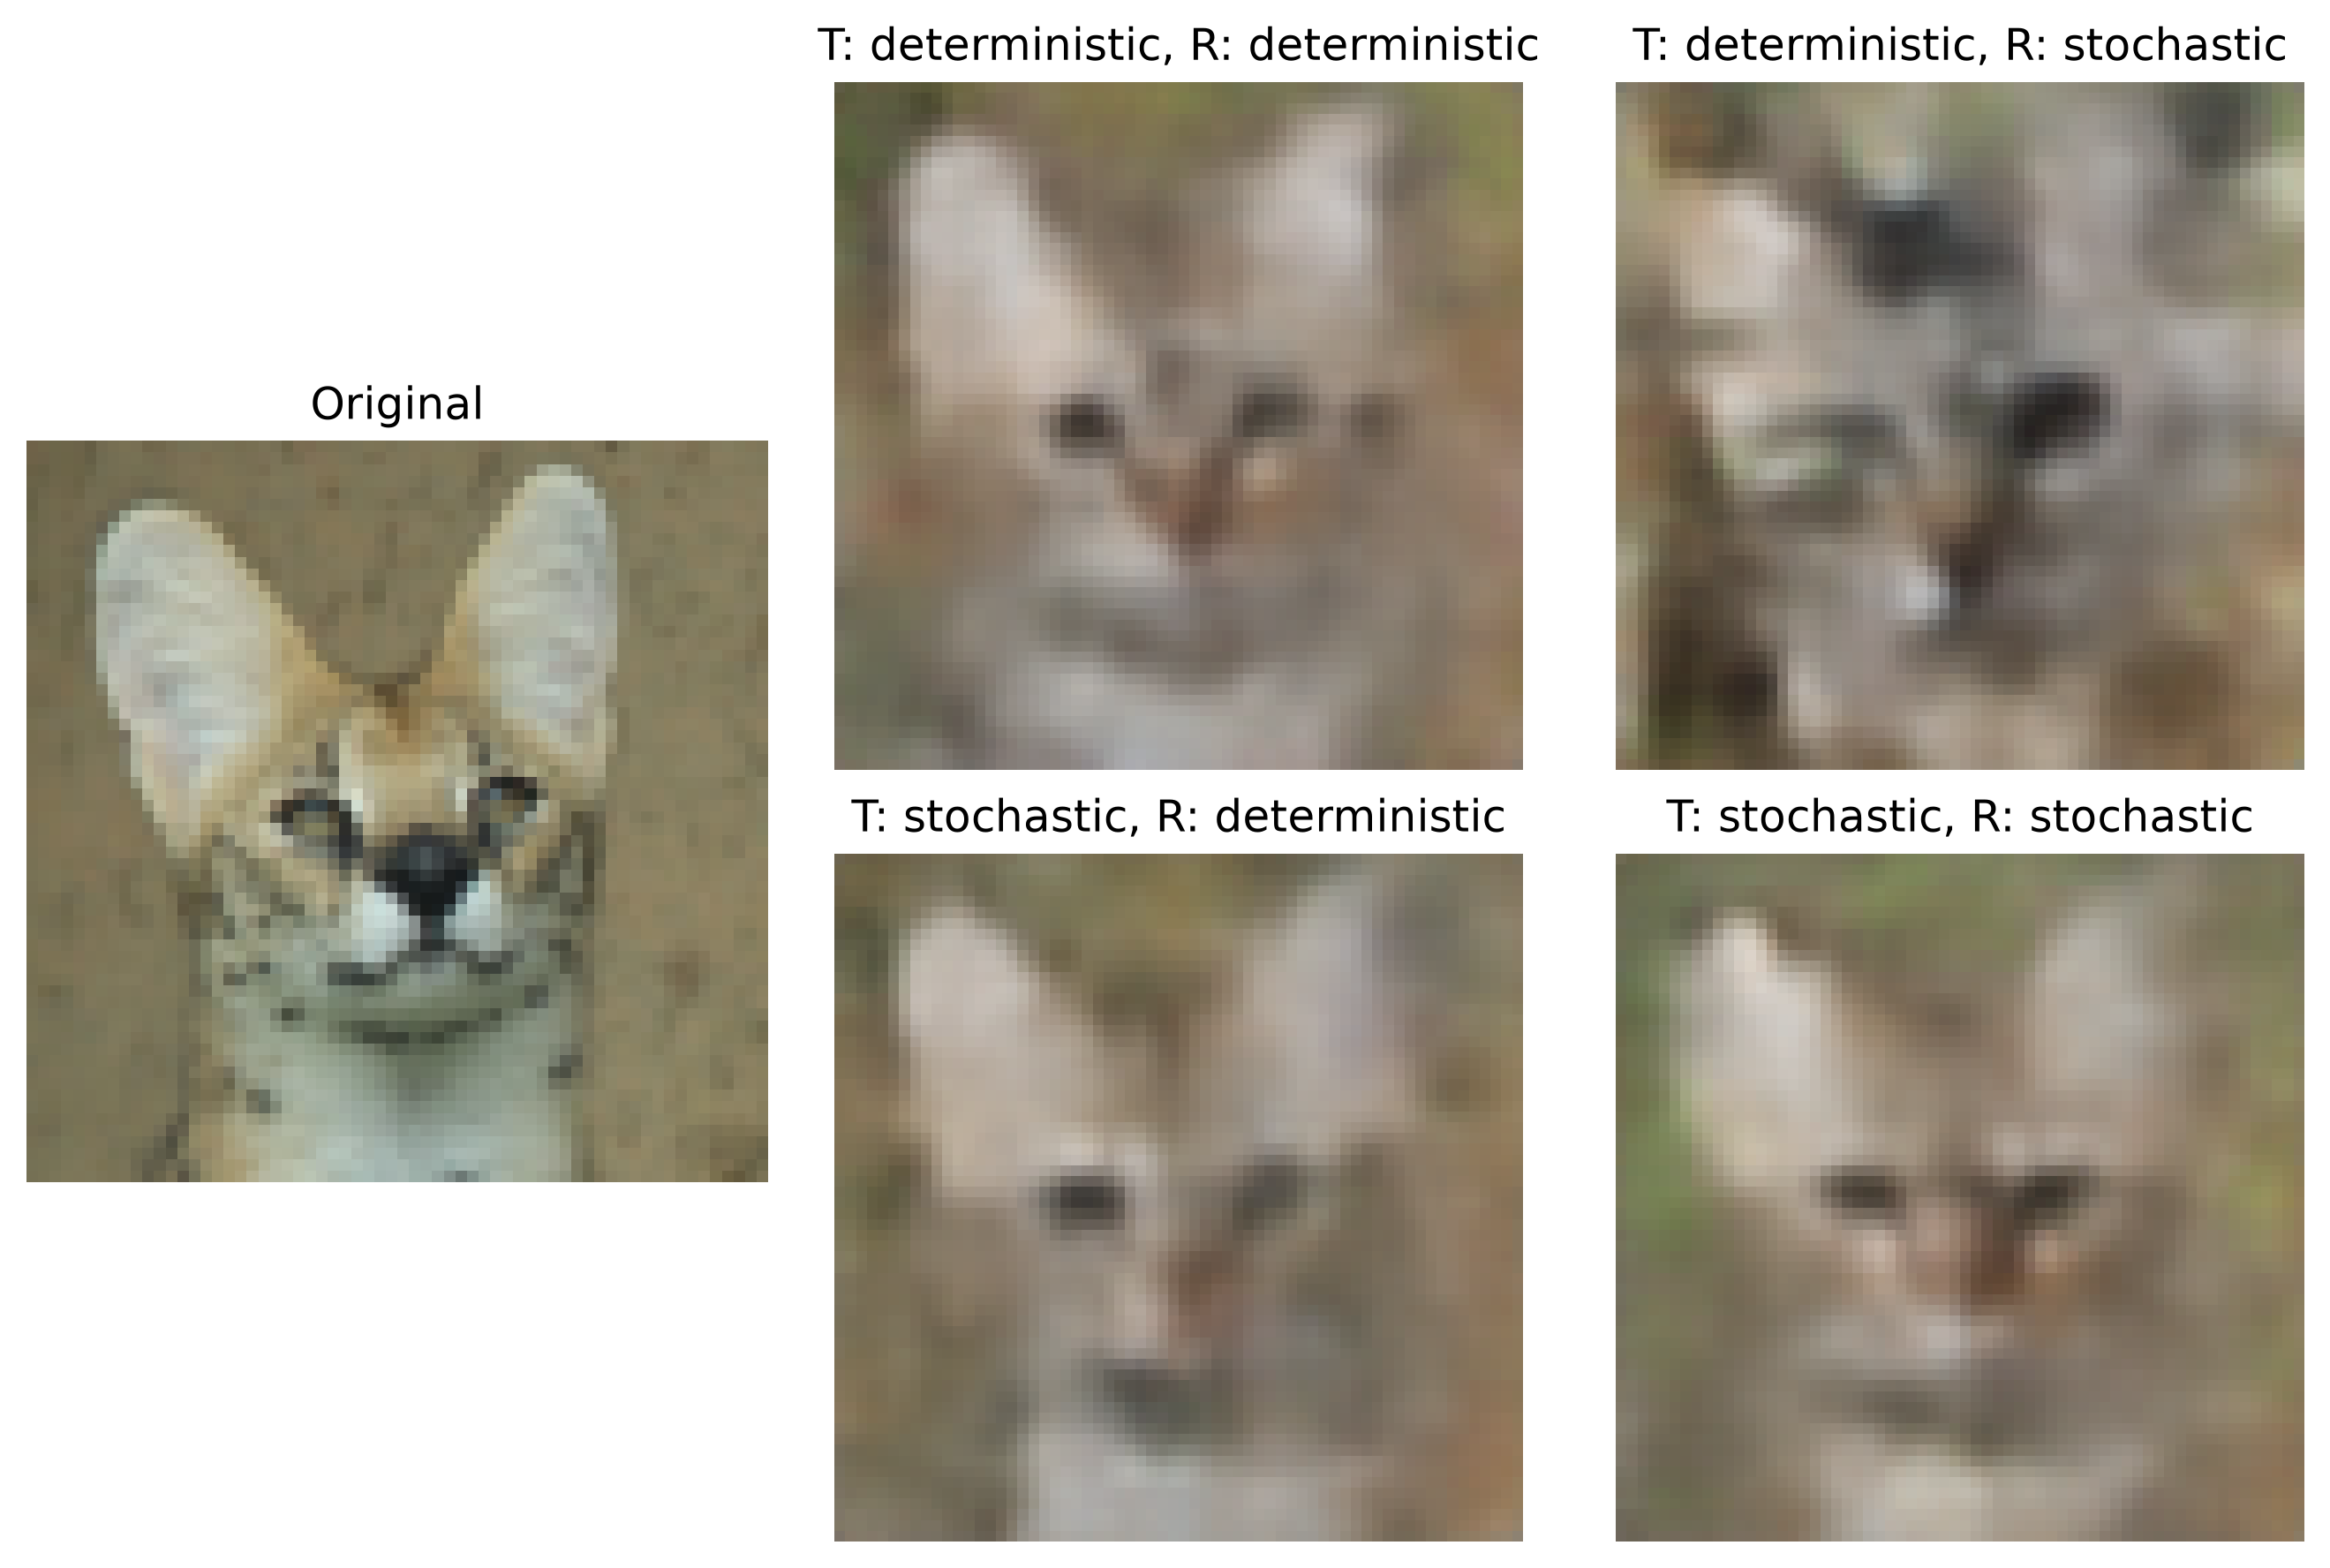
\includegraphics[width=\linewidth]{vector_latent/RQ2/full_dataset_100epok_beta0/reconstruction_grid_5.png}
        \caption*{}
    \end{subfigure}
\end{figure}

\begin{figure}[H]
    \centering

    \begin{subfigure}{0.48\textwidth}
        \centering
        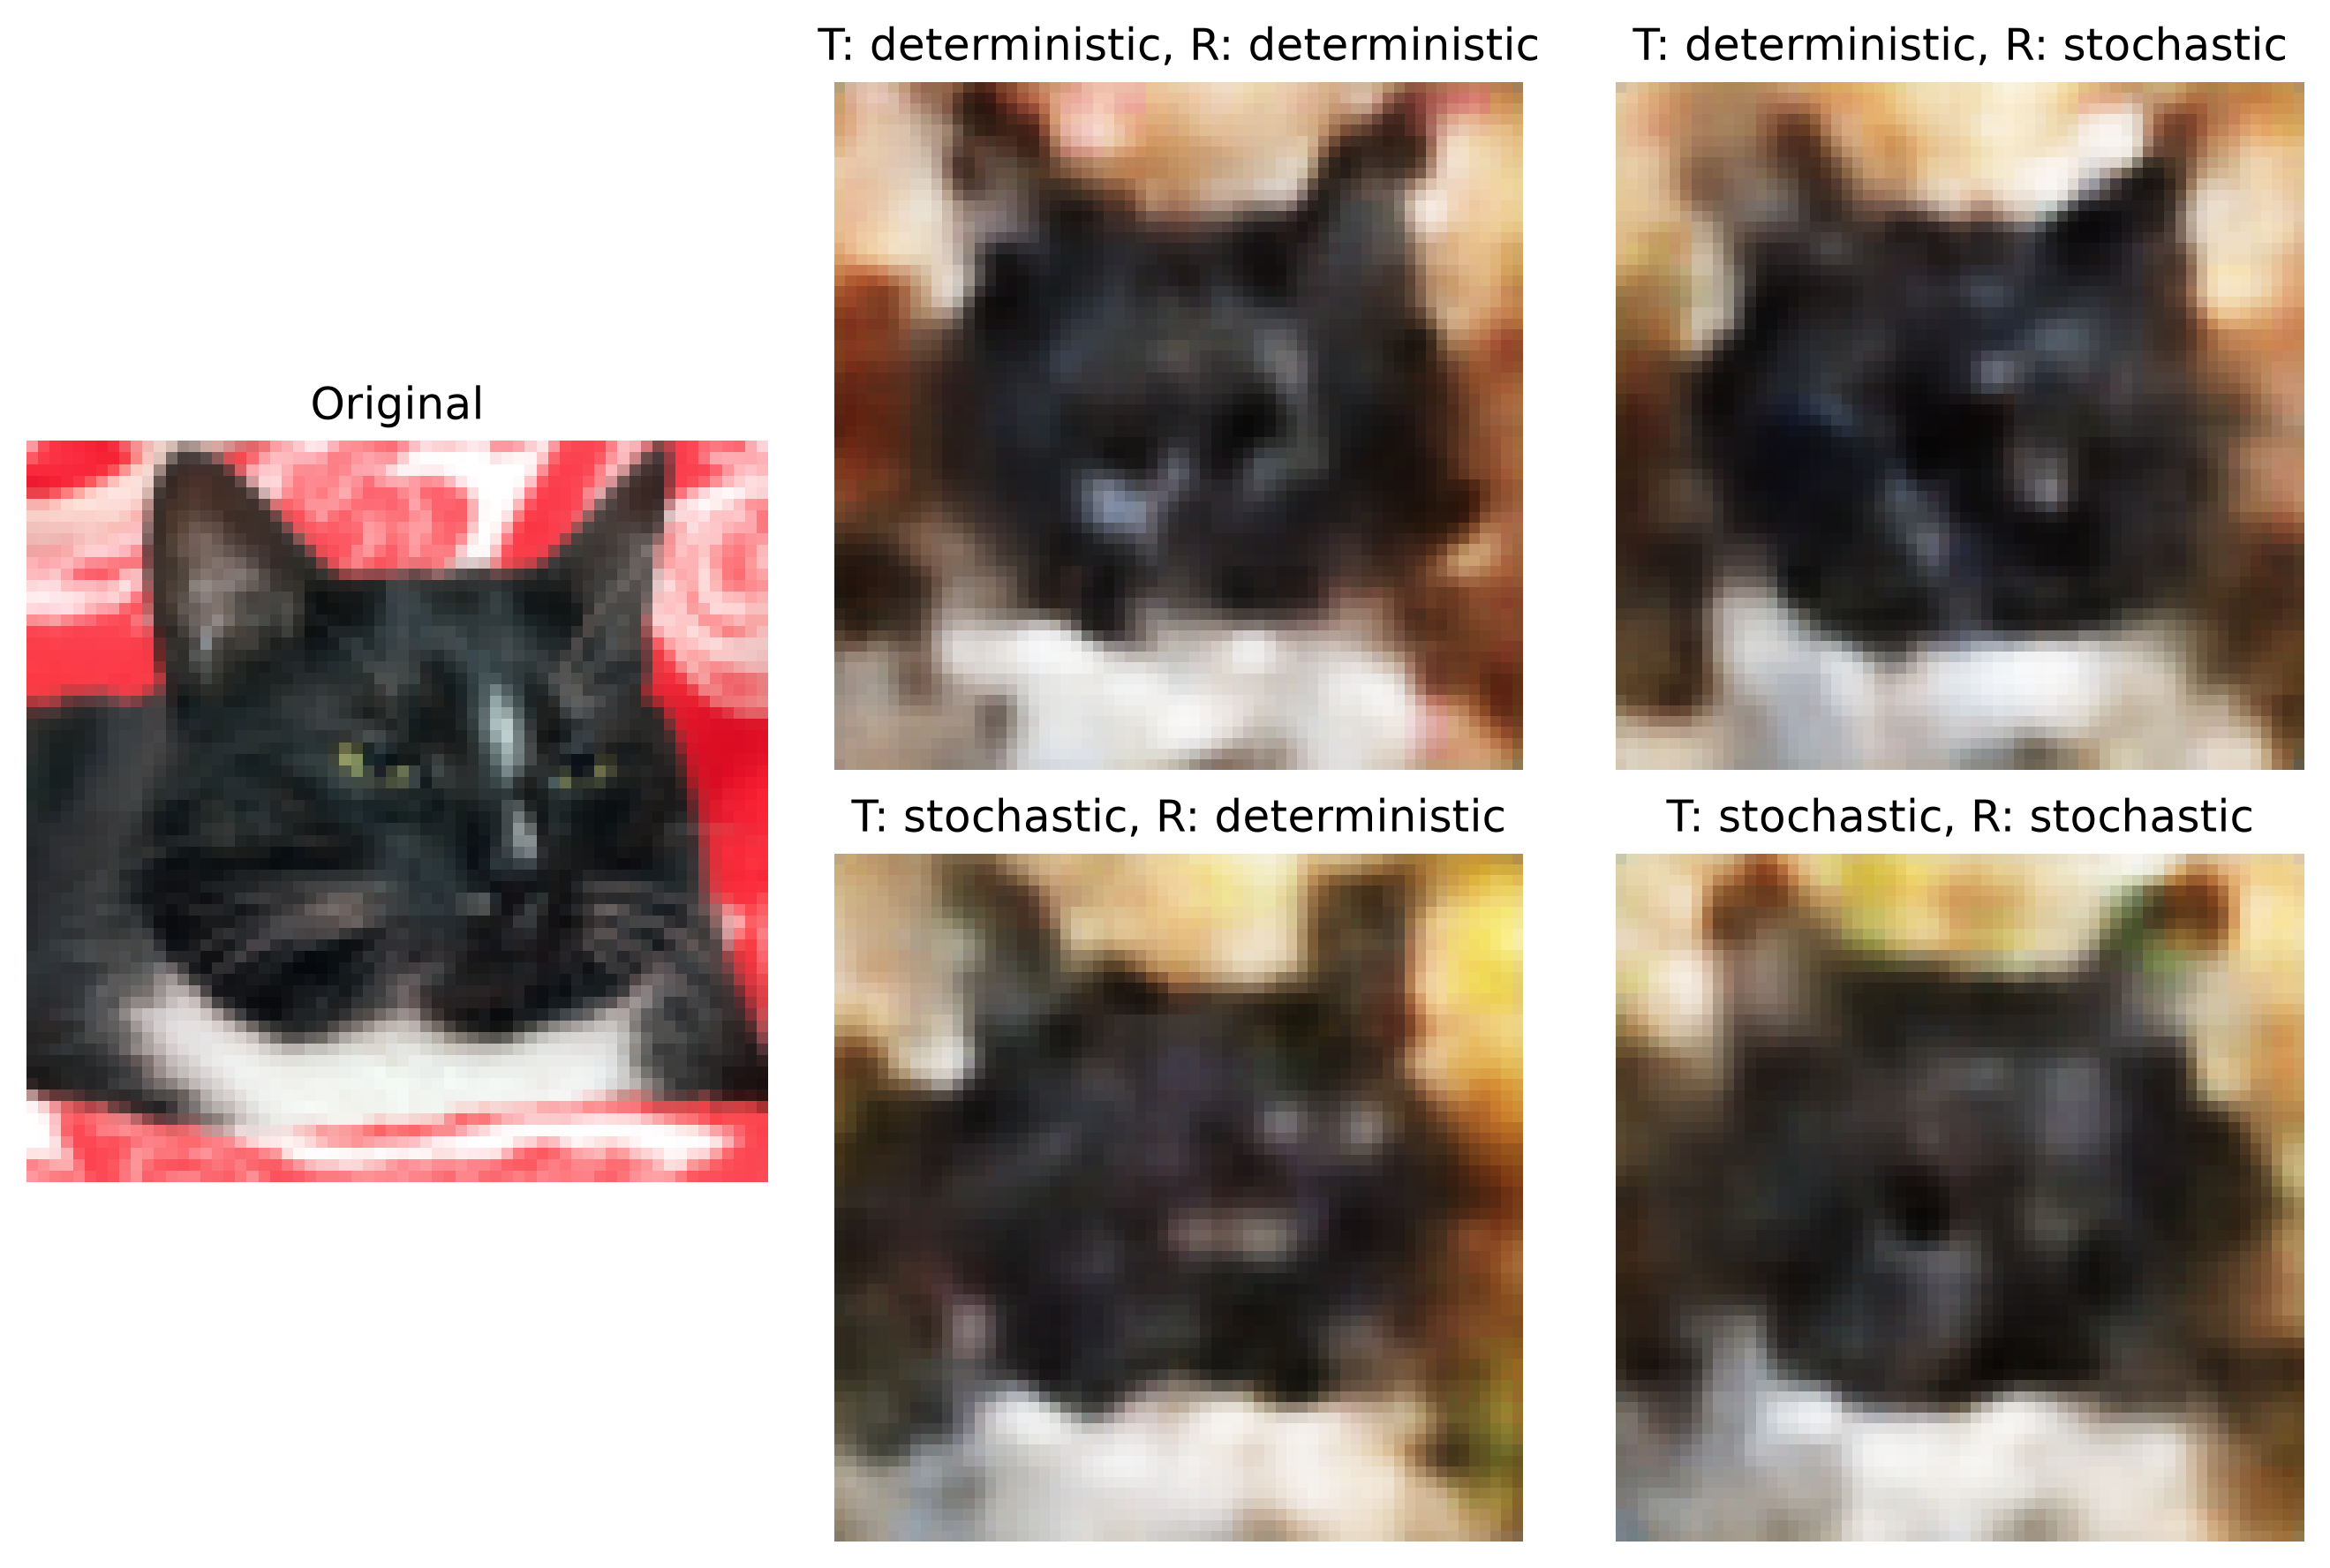
\includegraphics[width=\linewidth]{vector_latent/RQ2/full_dataset_100epok_beta0/reconstruction_grid_6.png}
        \caption*{}
    \end{subfigure}
    \hspace{0.02\textwidth}
    \begin{subfigure}{0.48\textwidth}
        \centering
        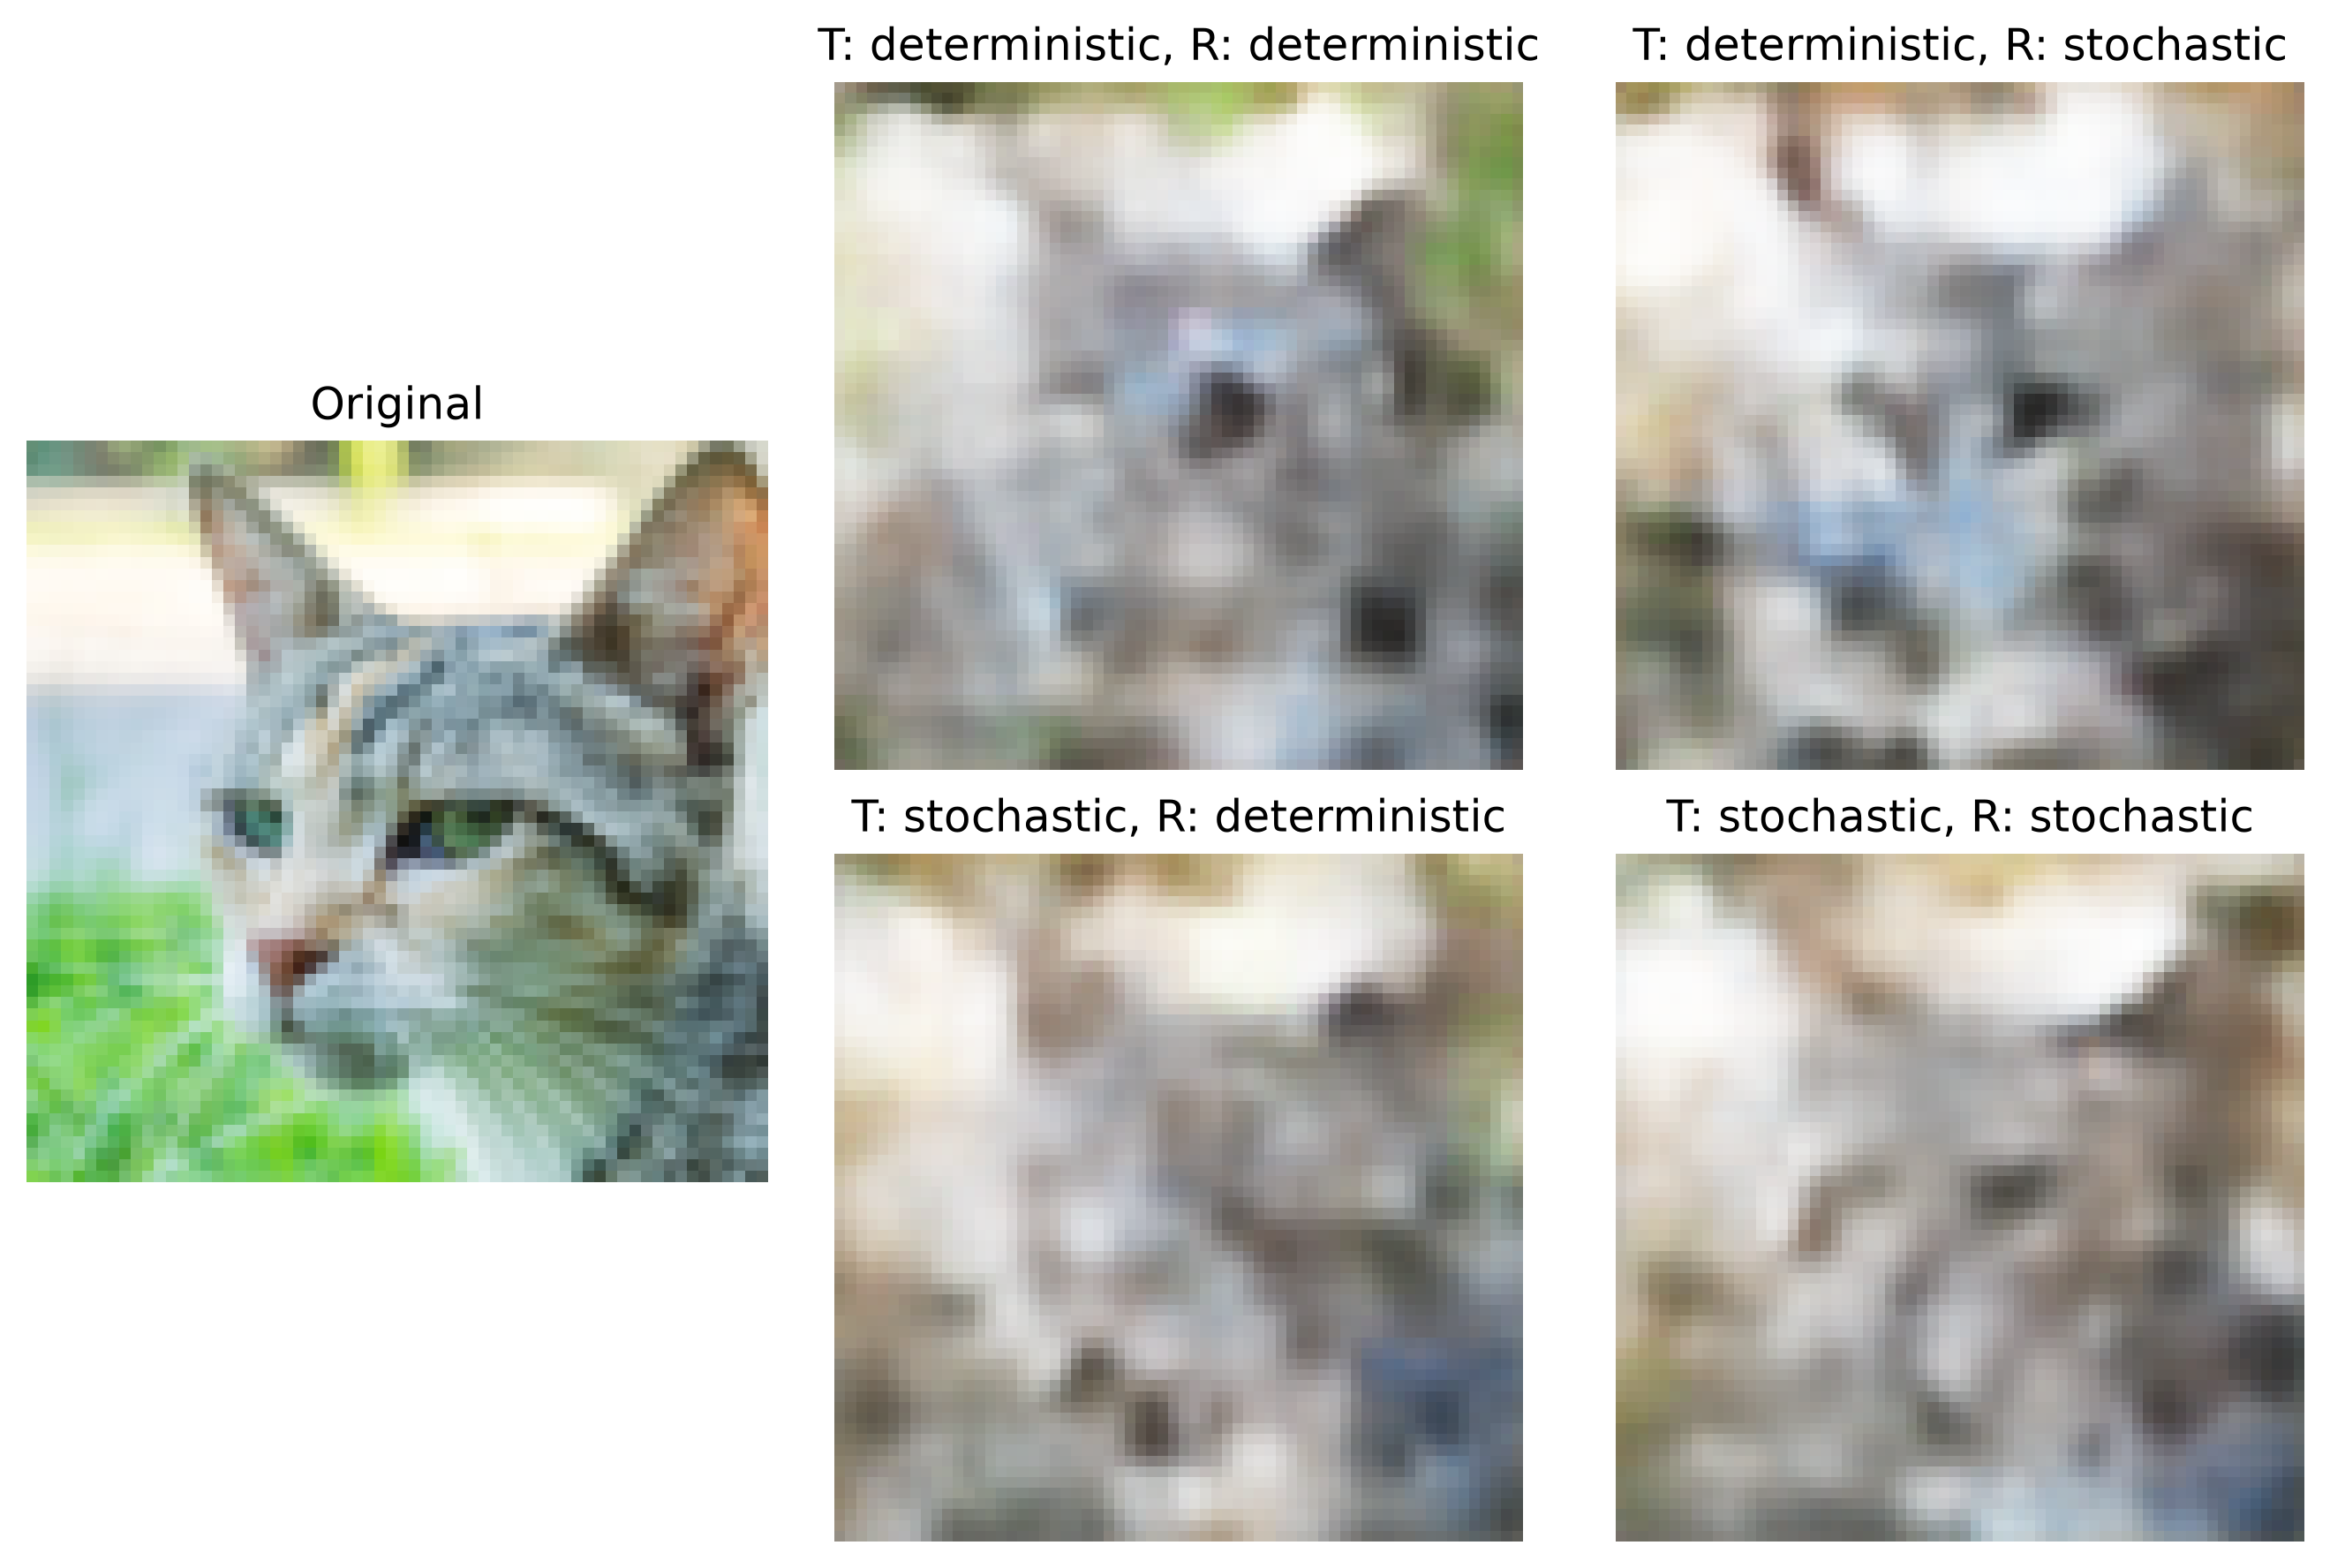
\includegraphics[width=\linewidth]{vector_latent/RQ2/full_dataset_100epok_beta0/reconstruction_grid_8.png}
        \caption*{}
    \end{subfigure}
\end{figure}

\textbf{Conclusion:} dataset complexity and limited representation capacity contribute to reconstruction blur independently of stochastic sampling and KL regularization.

\subsection{Latent Capacity without KL Regularization}

To investigate whether the latent bottleneck was limiting reconstruction quality, the full-dataset deterministic experiment was repeated with

\[
d_z \in \{64,128,256\},
\]

while keeping

\[
\beta=0
\qquad\text{and}\qquad
z=\mu.
\]

A substantial improvement was observed when increasing the latent dimensionality from

\[
64 \rightarrow 128.
\]

The reconstruction blur decreased noticeably and more image-specific details were preserved.

Increasing the latent dimensionality further from

\[
128 \rightarrow 256
\]

produced only a small additional improvement. The 256-dimensional model was slightly better than the 128-dimensional model, but the difference was much smaller than between 64 and 128 dimensions.

\textbf{Conclusion:} latent-space capacity is one of the factors contributing to reconstruction blur. A 64-dimensional representation appears to form a significant bottleneck for the full dataset, while the benefit of increasing the latent dimensionality becomes much smaller beyond approximately 128 dimensions.


\subsection{Interaction between Latent Capacity and KL Regularization}

An important difference was observed between the latent-capacity experiment without KL regularization and the earlier latent-dimensionality experiment with $\beta=1$.

Without KL regularization,

\[
64 \rightarrow 128
\]

produced a substantial improvement in reconstruction quality.

However, with $\beta=1$, increasing the latent dimensionality across

\[
d_z \in \{32,64,128,256\}
\]

produced very little visual improvement.

This result is consistent with the KL-per-dimension analysis. In larger latent spaces, many dimensions had

\[
D_{\mathrm{KL},j} \approx 0,
\]

meaning that the additional dimensions remained close to the prior and carried little additional information.

This suggests that the latent bottleneck itself is not the only problem. The amount of latent capacity that the model can effectively use also depends on the strength of KL regularization.

A larger latent space can improve reconstruction when the encoder is free to use it, but the same increase may provide little benefit when the KL term forces many dimensions toward the prior.

\textbf{Conclusion:}

\[
\boxed{
\text{nominal latent capacity}
\neq
\text{effective latent capacity}
}
\]

and reconstruction blur appears to depend partly on the interaction between latent dimensionality and KL regularization.


\section{Current Interpretation of the Reconstruction Blur Problem}

The experiments performed so far allow several simple explanations of reconstruction blur to be rejected.

The current evidence suggests that

\[
\text{blur}
\neq
\text{stochastic sampling alone},
\]

\[
\text{blur}
\neq
\text{Gaussian reconstruction loss alone},
\]

\[
\text{blur}
\neq
\text{a problem solved by SSIM alone},
\]

and

\[
\text{blur}
\neq
\text{KL regularization alone}.
\]

Instead, the results suggest that reconstruction blur is caused by an interaction between several factors:

\[
\boxed{
\text{dataset complexity}
+
\text{effective latent capacity}
+
\text{KL regularization}
}
\]

The small-dataset overfitting experiment showed that the model can produce relatively sharp reconstructions when only a limited number of images must be represented.

However, reconstruction quality decreased when the same approach was applied to the full dataset.

Increasing the latent dimensionality without KL regularization improved reconstruction quality, particularly when moving from

\[
d_z = 64
\]

to

\[
d_z = 128.
\]

At the same time, earlier experiments with $\beta=1$ showed very little improvement when increasing the latent dimensionality.

The KL-per-dimension analysis provides a possible explanation for this behaviour. In larger latent spaces, many dimensions remained close to

\[
D_{\mathrm{KL},j} \approx 0,
\]

which indicates that they carried little image-specific information.

Therefore, an important distinction must be made between nominal latent dimensionality and effective latent capacity:

\[
\boxed{
\text{nominal latent capacity}
\neq
\text{effective latent capacity}
}
\]

A larger latent vector can improve reconstruction when the encoder is free to use the additional dimensions. However, under KL regularization, some of this additional capacity may remain unused.

The current results therefore suggest that reconstruction blur is strongly related to the amount of information that can effectively pass through the latent representation while the model is simultaneously constrained to maintain a latent distribution suitable for prior sampling.

\section{Next Experiment: Latent Dimension vs. KL Weight}

The next controlled experiment will directly investigate the interaction between latent dimensionality and KL regularization.

The planned latent dimensions are

\[
d_z \in \{64,128,256\},
\]

and the KL weights are

\[
\beta \in \{0,0.1,0.5,1\}.
\]

KL annealing will not be used in this experiment. Each model will therefore use a constant value of $\beta$ throughout training.

All models will be trained under the same conditions and for the same number of epochs:

\[
50 \text{ epochs}.
\]

Models will be compared at the same training epoch rather than selecting a different best checkpoint for each configuration. This keeps the training budget constant and avoids introducing training duration as an additional variable.

The experiment therefore consists of the following parameter grid:

\begin{table}[h]
\centering
\begin{tabular}{c|ccc}
\hline
 & $d_z=64$ & $d_z=128$ & $d_z=256$ \\
\hline
$\beta=0$   & model & model & model \\
$\beta=0.1$ & model & model & model \\
$\beta=0.5$ & model & model & model \\
$\beta=1$   & model & model & model \\
\hline
\end{tabular}
\caption{Planned comparison of latent dimensionality and KL regularization strength.}
\label{tab:latent_beta_grid}
\end{table}

The main research question for this experiment is:

\begin{quote}
Does reducing KL regularization allow larger latent spaces to use their additional capacity while still preserving meaningful generation from the prior?
\end{quote}


\section{Planned Model Improvements}

After the latent-dimension and KL-weight experiment, the next step will be to investigate whether increasing model capacity can further reduce the remaining blur.

The current CNN VAE can already produce relatively sharp reconstructions in the small-dataset overfitting experiment, but it may still have insufficient capacity to efficiently represent the full dataset under a regularized VAE objective.

Possible modifications include:

\begin{itemize}
    \item increasing network depth,
    \item increasing the number of feature channels,
    \item introducing residual blocks,
    \item testing normalization layers such as Group Normalization,
    \item replacing some transposed convolutions with upsampling followed by standard convolution.
\end{itemize}

Residual blocks are particularly interesting because they allow deeper feature processing while providing skip connections that improve gradient flow.

The final objective is not necessarily to obtain perfectly sharp reconstructions. The main goal is to construct a VAE that can generate recognizable and diverse cat images from the prior while keeping reconstruction and generation blur relatively small:

\[
\boxed{
\text{meaningful prior generation}
+
\text{moderate blur}
+
\text{effective use of latent information}
}
\]

\end{document}
